\documentclass[mathserif]{beamer}
\usepackage{beamerthemeshadow}
\usepackage{beamerthemesplit}
%\usetheme{shadow}
\usecolortheme{default}
\setbeamertemplate{footline}[frame number]
\useinnertheme[shadow=true]{rounded}
%\setbeamertemplate{footline}{\insertframenumber/\inserttotalframenumber}
%\useoutertheme{infolines}
%\setbeamertemplate{headline}{} % removes the headline that infolines inserts

%\usetheme{boxes}
%\usepackage{amsmass}
%\usepackage{amssymb,amsfonts,url}

\usepackage{algorithm}
\usepackage{algorithmic}

\usepackage{graphicx}
\graphicspath{{Problems/}}
\usepackage{subfigure}
%\usepackage{CJK}
%\usepackage{pinyin}

\usepackage{tikz}
\usepackage{verbatim}
\usepackage{pgfplots}
\usepackage{verbatim}
\usetikzlibrary{arrows,shapes}

\tikzstyle{vertex}=[circle,fill=black!25,minimum size=20pt,inner sep=0pt]
\tikzstyle{smallvertex}=[circle,fill=black!25,minimum size=10pt,inner sep=0pt]
\tikzstyle{middlevertex}=[circle,fill=black!25,draw,minimum size=15pt,inner sep=0pt]
\tikzstyle{selected vertex} = [vertex, fill=red!24]
\tikzstyle{blue smallvertex} = [smallvertex, fill=blue]
\tikzstyle{red smallvertex} = [smallvertex, fill=red]
\tikzstyle{edge} = [draw,thick,->]
\tikzstyle{undirectededge} = [draw,thick]
\tikzstyle{weight} = [font=\small]
\tikzstyle{selected edge} = [draw,line width=5pt,-,red!50]
\tikzstyle{ignored edge} = [draw,line width=5pt,-,black!20]



\title{CS711008Z  Algorithm Design and Analysis }
\subtitle{ Lecture 3. Problem hardness and polynomial-time reduction 
%	\footnote{The slides are prepared based on Introduction to algorithms, Algorithm design, and Computer and Intractability.} 
}
\author{Dongbo Bu \\
\ \ \ \ \ \ \ \ \ \ \ \ \ \ \ \ \ \ \ \ \ \ \ \ \ \ \ \ \ \ \ \ \ \ \ \ \ \ \ \ \ \ \ \ \ \ \ \ \ \ \ \ \ \ \ \ \ \ \ \ \ \ \ \ \ \ \ \ \ \ \ \ \ \ \ \ \ \ \ \ \ \ \ \ \ \ \ \ \ \ \ \ \ \ \ \ \ \ \ \  \\
{\small Institute of Computing Technology \\ Chinese Academy of Sciences, Beijing, China}
}
\date{}

\begin{document}
%\begin{CJK}{UTF8}{cyberbit}

\frame{\titlepage}


\frame{
\frametitle{Outline}
\begin{itemize}
 \item Problem intrinsic property: hardness
 \item Reduction: to identify the relationship between different problems; 
\end{itemize}
}

\frame{
\frametitle{NP-Completeness Cartoon: Bandersnatch problem  }
\begin{itemize}
 \item 


One day your boss calls you into his office and confides that the company is about to enter the highly competitive "bandersnatch" market. 

\item
A good method is needed for determining whether or not any given set of specifications for a new bandersnatch component can be met and, if so, for constructing a design that meets them. 

\item
Since you are the company's chief algorithm official, your charge is to find an efficient algorithm for doing this.
\end{itemize}
\footnote{Excerpted from Computer and Intractability (by Garey and Johnson)}

}


\frame{
\frametitle{Trial 1: attempt to solve this problem}
\begin{itemize}
 \item 


Some weeks later, you have not been able to come up with any algorithm substantially better than searching through all possible designs. This would involve years of computation time for just one set of specifications. 

\item
You simply return to your boss's office and report: ``I can't find an efficient algorithm, I guess I'm just too dumb. ''
\begin{figure}
        \centering
        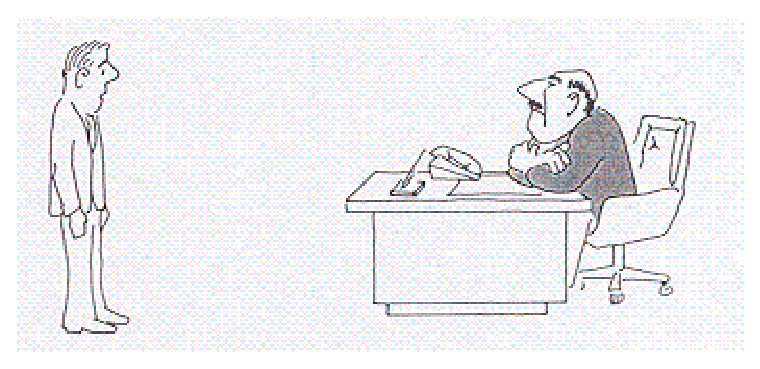
\includegraphics[width=2in]{L3-NPCartoon1.eps}
\end{figure}

\item But perhaps this is unfair to you: \textcolor{red}{ the problem might be intrinsically hard. }
\end{itemize}

}

\frame{
\frametitle{Trial 2: try to prove the hardness directly}
\begin{itemize}
 \item 

So it would be much better if you could prove that the bandersnatch problem is inherently intractable, that no algorithm could possibly solve it quickly. 

\item
Then you could stride confidently into the boss's office and proclaim: \textcolor{red}{`` I can't find an efficient algorithm, 
because no such algorithm is possible. ''}

\begin{figure}
        \centering
        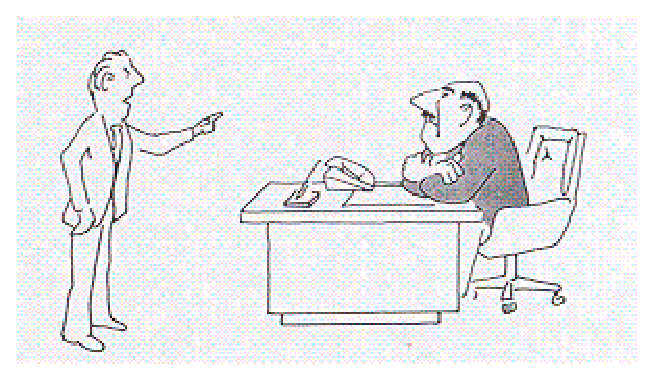
\includegraphics[width=1.85in]{L3-NPCartoon2.eps}
\end{figure}

\item Unfortunately, proving inherent intractability can be just as hard as finding efficient algorithms. 
\end{itemize}
}

\frame{
\frametitle{Trial 3: to show the relative hardness with other hard problems  }
\begin{itemize}
 \item 

 For such a ``grey area'' problem, an alternative way is to prove that the problem is ``just as hard as'' a large number of other problems that are widely recognize as being difficult and that have been confounding the experts for years.

\item
 \textcolor{red}{``I can't find an efficient algorithm, but neither can all these famous people. '' }
\end{itemize}
\begin{figure}
        \centering
        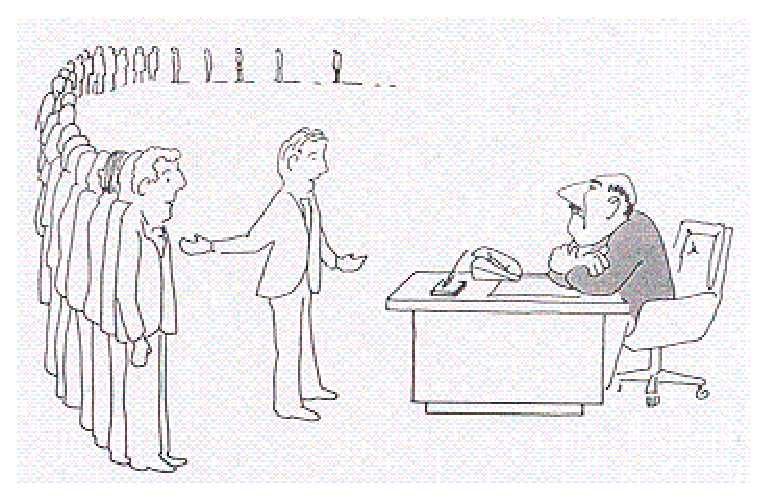
\includegraphics[width=1.5in]{L3-NPCartoon3.eps}
\end{figure}
}

\frame{
\frametitle{Trial 3: to show the relative hardness with other hard problems. cont'd }
\begin{itemize}
\item Two advantages: 
\begin{enumerate}

\item  At the very least, this would inform your boss that it would do no good to fire you and hire another expert on  algorithms. 

\item  More importantly, you can spend your time looking for efficient algorithms that solve various special cases of the general problem. 
\end{enumerate}
\end{itemize}
}

\frame{
\begin{block}{}
 Problem and its hardness
\end{block}
}

\frame{
\frametitle{Hardness or complexity: an intrinsic property of problem }
\begin{itemize}
\item 
Problems can be:
\begin{itemize}
 \item  Easy (existing polynomial-time algorithm): {\sc StableMatching} problem;
 \item  NP-hard: {\sc Satisfiability} problem; 
 \item  Truly hard (provably non-polynomial, exponential): Given a Turing machine, does it halt in  at most $k$ steps? 
 \item  Impossible: {\sc HALT} problem
\end{itemize}
\end{itemize}
}

\frame{
\frametitle{Abstracting problem}


\begin{itemize}
 \item 
Problem: consisting of \texttt{INPUT} and \texttt{OUTPUT} parts. \\
 Formally, a problem can be described as a {\it relation} $P   \subseteq I\times S$, where $I$ denotes the {\bf problem input}, and $S$ denotes the set of problem {\bf solutions}. \\
\item Instance: a particular \texttt{INPUT}. 
\end{itemize}

} 

\frame{ 
 \frametitle{An example }
\begin{itemize}
\item {\sc s-t connectivity} problem

\begin{block}{}
{\bf INPUT:} a graph $G=<V,E>$, two vertices $s$, and $t$; \\
{\bf OUTPUT:} a path from $s$ to $t$; ( or ``NO'' if there is no such path)
\end{block}
\item 
Instance: a particular \texttt{INPUT}, including $G$, and $s$, $t$. 

\begin{figure}[H]
\center
\begin{tikzpicture}[scale=1.3, auto,swap]
    % Draw a 7,11 network
    % First we draw the vertices
    % Connect vertices with edges and draw weights
        \foreach \pos/\name in {{(0,0)/s}, {(2,1)/u}, {(2,-1)/v}, {(4,0)/t}}
       	 	\node[middlevertex, draw,  fill=blue!20] (\name) at \pos {$\name$};
    
    \foreach \source/ \dest /\weight in {s/u/{1/2}, u/t/{ 0/2},u/v/{1/3},s/v/{0/1},      v/t/{1/1} }
        \path[edge, sloped, midway, below, allow upside down] (\source) -- node[weight] {$\weight$} (\dest);
    \path[draw, thick, ->, blue] (0, 0) -- (2,1);
         \path[draw, thick, ->, blue] (2,1) -- (2,-1);
             \path[draw, thick, ->, blue] (2, -1) -- (4, 0);


   \end{tikzpicture}
\end{figure}

%  \begin{figure}
%  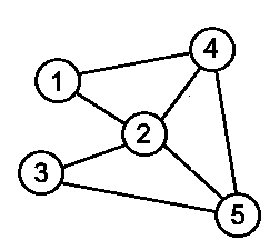
\includegraphics[width=1in]{L3-connectivity.png}
%  \end{figure}
 \end{itemize} 
}

\frame{
\frametitle{Two types of problems: Optimization problem}
\begin{itemize}
 \item 
Optimization problem: given an instance $x \in I$, to find the ``best'' solution $y^*$ according to some measure. 
\item 
Example: {\sc Shortest-Path} problem

\begin{block}{}
{\bf INPUT:}  a graph $G=<V,E>$, two vertices $s$, and $t$; \\
{\bf OUTPUT:}  the shortest path from $s$ to $t$, or ``NO'' if there is no path from $s$ to $t$;
\end{block}
\end{itemize}

%\begin{figure}
%  \includegraphics[width=1.0in]{L3-shortestpath.jpg}
%\end{figure}

}

\frame{
\frametitle{Two types of problems: Decision problem}
\begin{itemize}
 \item 
Decision problem: the relation $P   \subseteq I\times S$ reduces to a function $f: I \mapsto S$, where $S=\{ \texttt{YES, NO} \}$.
\item


Example: {\sc Path} problem
\begin{block}{}
{\bf INPUT:} a graph $G=<V,E>$, two vertices $s$, and $t$, and \textcolor{red}{an integer $k$};\\
{\bf OUTPUT:} a path from $s$ to $t$ with length at most $k$; 
\end{block}
\end{itemize} 

%\begin{figure}
%        \centering
%        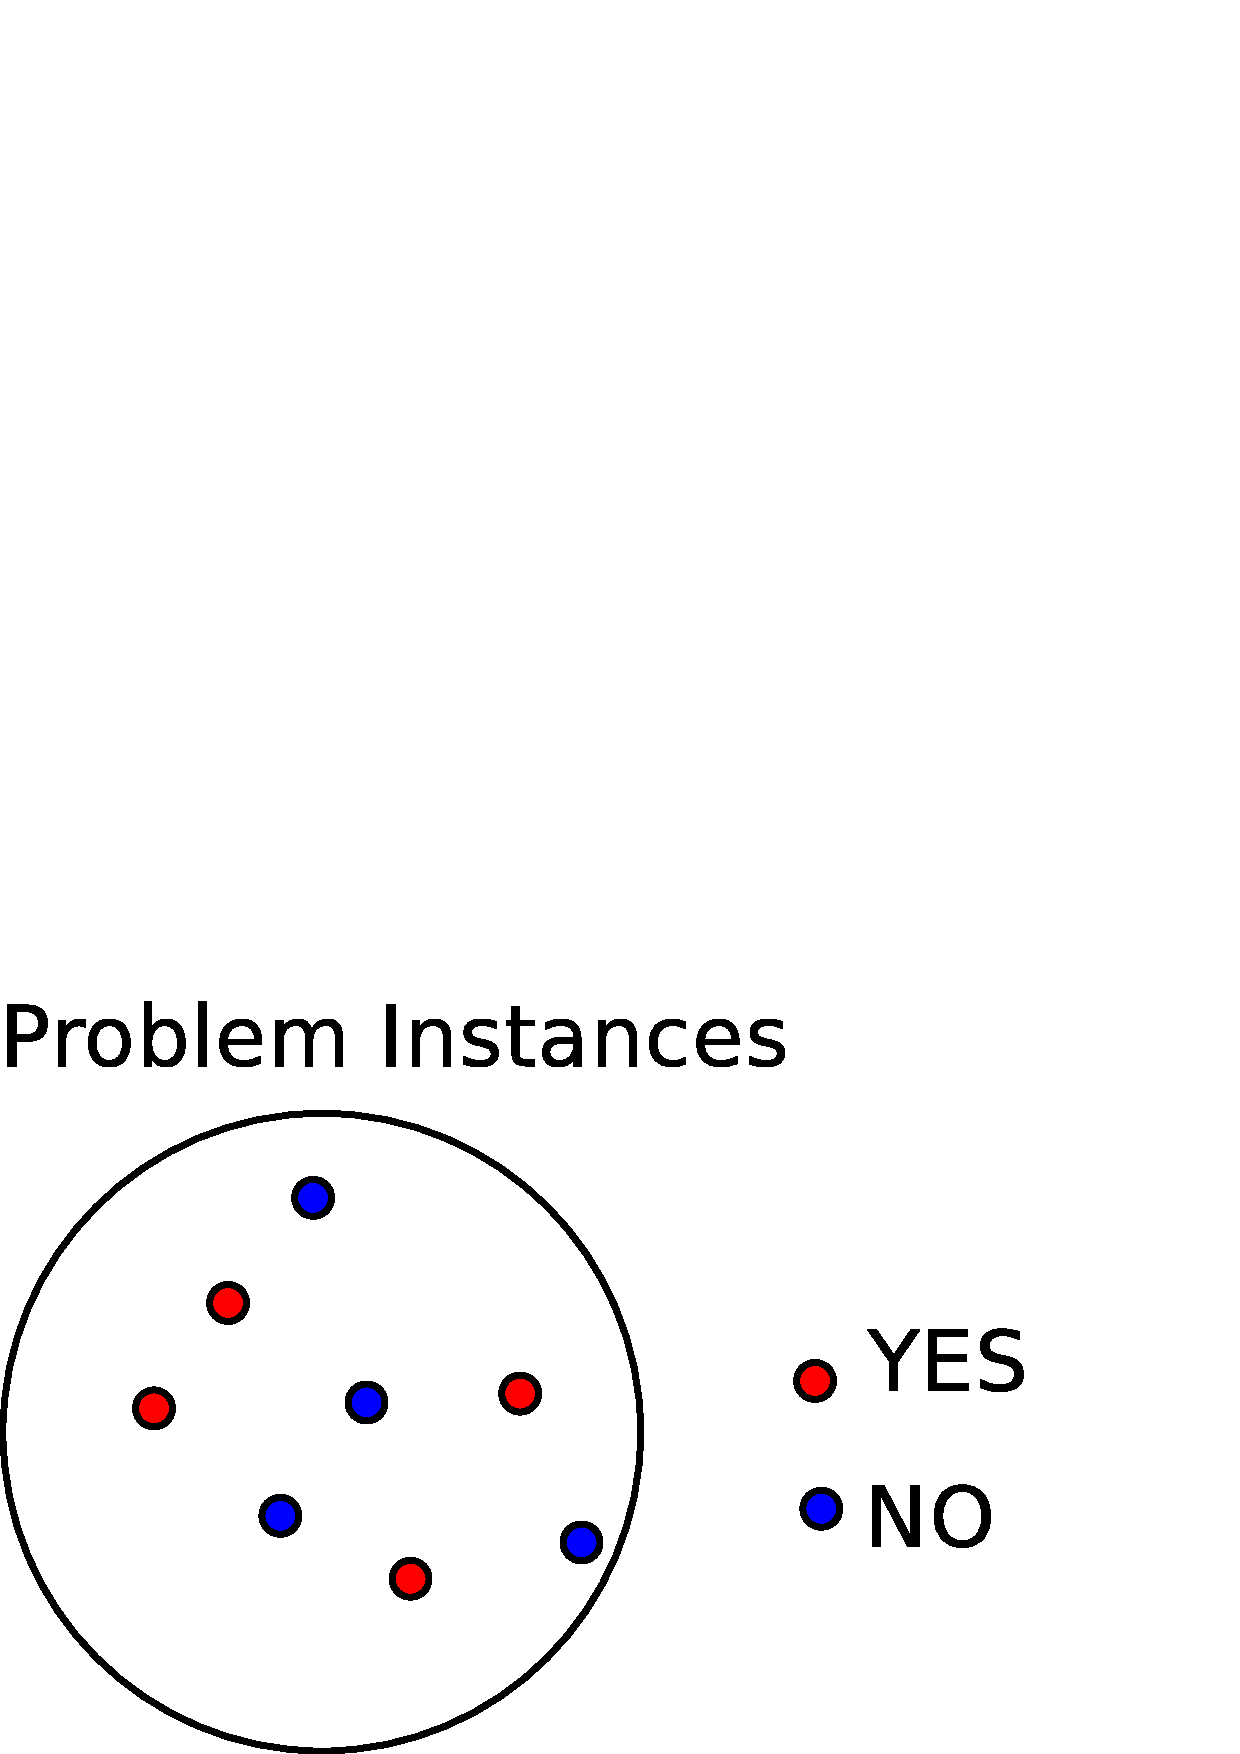
\includegraphics[width=1.5in]{L3-decisionproblem.png}
%\end{figure}
}

\frame{
\frametitle{The relationship between decision problem  and optimization problem}
\begin{itemize}
 \item The decision problem is in a sense ``easier''. \\
\item
An optimization problem can be cast to a related decision problem by \textcolor{red}{\bf imposing a bound of the value to be optimized.} 
\item 
 For example, we can solve the {\sc Path} problem by solving the {\sc Shortest Path} problem, and then comparing the length of the shortest path with the decision problem parameter $k$. \\
% \item Conversely, we can solve the optimization problem through solving the decision problem;
\end{itemize}
}


\frame{
\frametitle{Reduction: uncovering the connection between two problems}
\begin{itemize}
 \item 


{\sc Polynomial-time reduction}: a procedure $f$ to transform \textcolor{red}{\bf any} instance $\alpha$ of problem $A$ to some instance $\beta=f(\alpha)$ of problem $B$ with the following characteristics: 
\begin{enumerate}
 \item  \textcolor{blue}{\bf Transformation}: The transformation takes polynomial time; \\
\item  \textcolor{blue}{\bf Equivalence}: The answers are the same, i.e. the answer for $\alpha$ is  \texttt{YES} iff the answer to $\beta=f(\alpha)$ is also \texttt{YES}.
\end{enumerate} 
\item  
Denoted as $A \leq_P B$, read as  ``\textcolor{red}{\bf A is reducible to  B  }''.
\end{itemize}

\begin{figure}
        \centering
        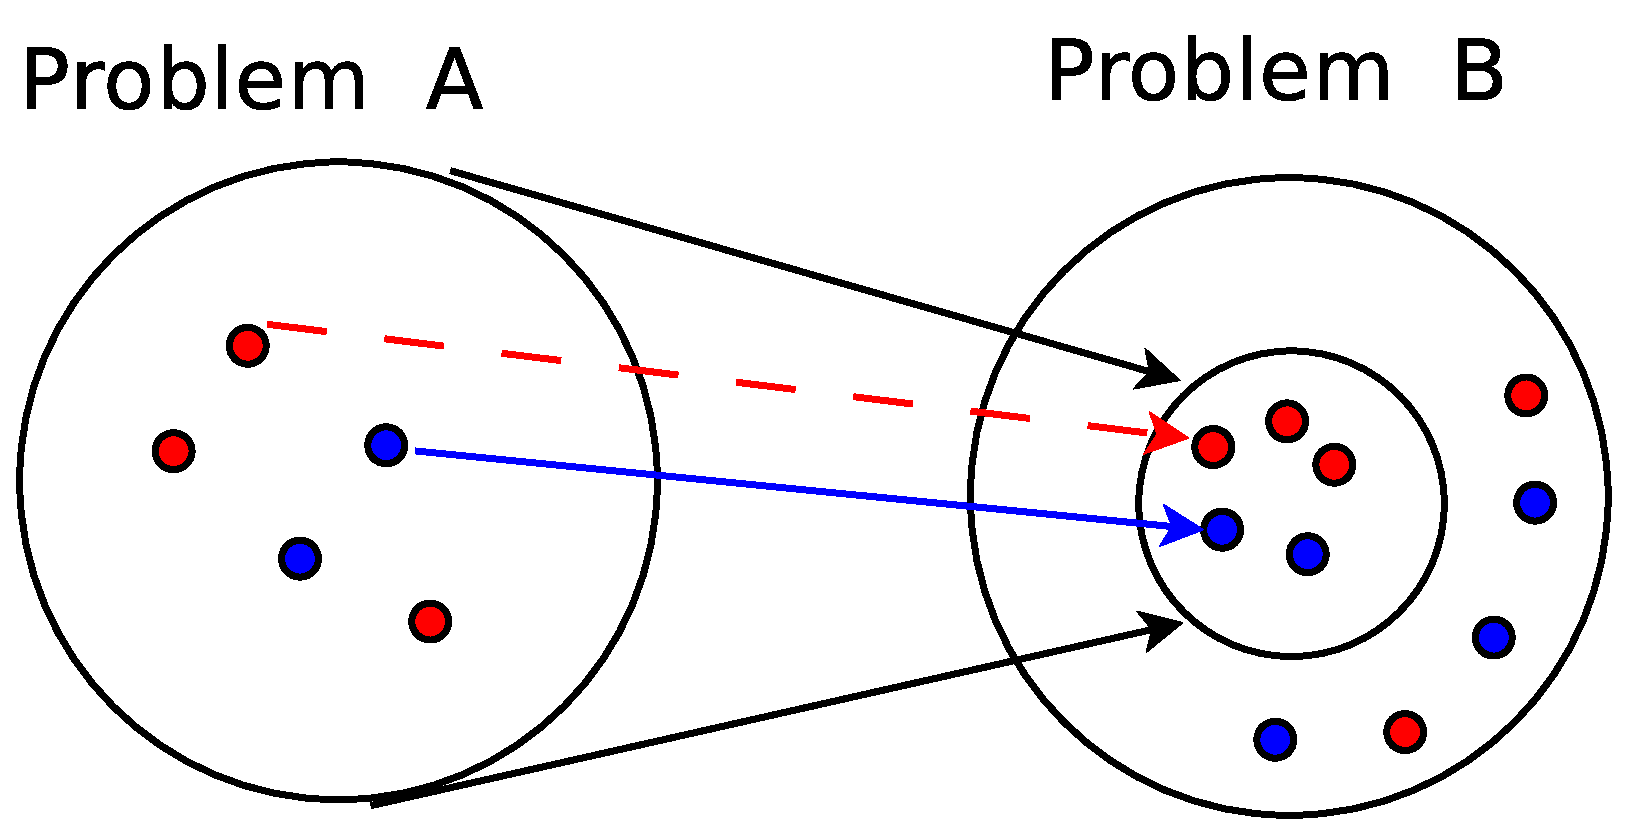
\includegraphics[width=2in]{L3-reduction.eps}
\end{figure}
}

\frame{
\frametitle{The significance of polynomial-time reduction}

\begin{theorem}
 If $B$ can be solved in polynomial time, $A$ is also polynomially solvable. 
\end{theorem}
The algorithm to problem $A$ is described as follows:\\

 \begin{algorithmic}[1]
 \STATE  Given an instance $\alpha$ of problem $A$, use polynomial-time reduction to transform it to $\beta=f(\alpha)$; 
 \STATE Run the polynomial-time algorithm for $B$ on the instance $\beta=f(\alpha)$;
 \STATE Use the answer to $\beta$ as the answer to $\alpha$. 
 \end{algorithmic}
\begin{theorem}
Conversely, if $A$ is hard, then $B$ is hard, too.  
\end{theorem}
}




\frame{
\frametitle{}
\begin{block}{}
 A simple reduction: {\sc IndependentSet} $\le_P$ {\sc VertexCover}
\end{block}
}


\frame{
\frametitle{ {\sc Independent Set} Problem}
\begin{itemize}
 \item 
Practical problem: \\ {\em 
 	Suppose you have $n$ friends, and some pairs of them don't get along. How to invite at least $k$ of them to dinner if you don't want any interpersonal tension? }

\begin{block}{Formalized Definition: }
 {\bf Input:} Given a graph $G=<V,E>$, and an integer $k$, \\
 {\bf Output:} is there a set of nodes $S  \subseteq V$, $|S| = k$, such that no two nodes in $S$ are joined by an edge?
\end{block}

\item An example: are there 3 independent nodes in the following graph?
\begin{figure}
\begin{tikzpicture}[scale=1.1, auto,swap]
    % Draw a 7,11 network
    % First we draw the vertices
    \foreach \pos/\name in {{(0,2)/v1}, {(2,2)/v2}, {(1,1)/v3}, {(2,1)/v4}, {(3,1)/v5}, {(0,0)/v6}, {(2,0)/v7}}
        \node[smallvertex] (\name) at \pos {};
        
    % Connect vertices with edges and draw weights
    \foreach \source/ \dest /\weight in {v1/v2/{}, v1/v3/{}, v2/v3/{}, v2/v4/{}, v2/v5/{}, v3/v6/{}, v3/v7/{}, v6/v7/{}, v4/v7/{}, v5/v7/{}  }
        \path[undirectededge] (\source) -- node[weight] {$\weight$} (\dest);
%       \draw[dashed, ->] (0,0) arc  (120:60:2);

      \end{tikzpicture}

\end{figure}

\end{itemize}
}

\frame{
\frametitle{ An example}



\begin{figure}
\begin{tikzpicture}[scale=1.1, auto,swap]
    % Draw a 7,11 network
    % First we draw the vertices
    \foreach \pos/\name in {{(0,2)/v1}, {(2,2)/v2}, {(1,1)/v3}, {(2,1)/v4}, {(3,1)/v5}, {(0,0)/v6}, {(2,0)/v7}}
        \node[smallvertex] (\name) at \pos {};
        
    % Connect vertices with edges and draw weights
    \foreach \source/ \dest /\weight in {v1/v2/{}, v1/v3/{}, v2/v3/{}, v2/v4/{}, v2/v5/{}, v3/v6/{}, v3/v7/{}, v6/v7/{}, v4/v7/{}, v5/v7/{}  }
        \path[undirectededge] (\source) -- node[weight] {$\weight$} (\dest);
%       \draw[dashed, ->] (0,0) arc  (120:60:2);


    \foreach \pos/\name in { {(1,1)/v3}, {(2,1)/v4}, {(3,1)/v5}}
        \node[blue smallvertex] (\name) at \pos {};
      \end{tikzpicture}


\end{figure}
\begin{itemize}
\item The three nodes in blue are independent.

\end{itemize}
}




\frame
{
\frametitle{Independent Set -- another interesting instance}

\begin{figure}
 \begin{minipage}{0.45\textwidth}
 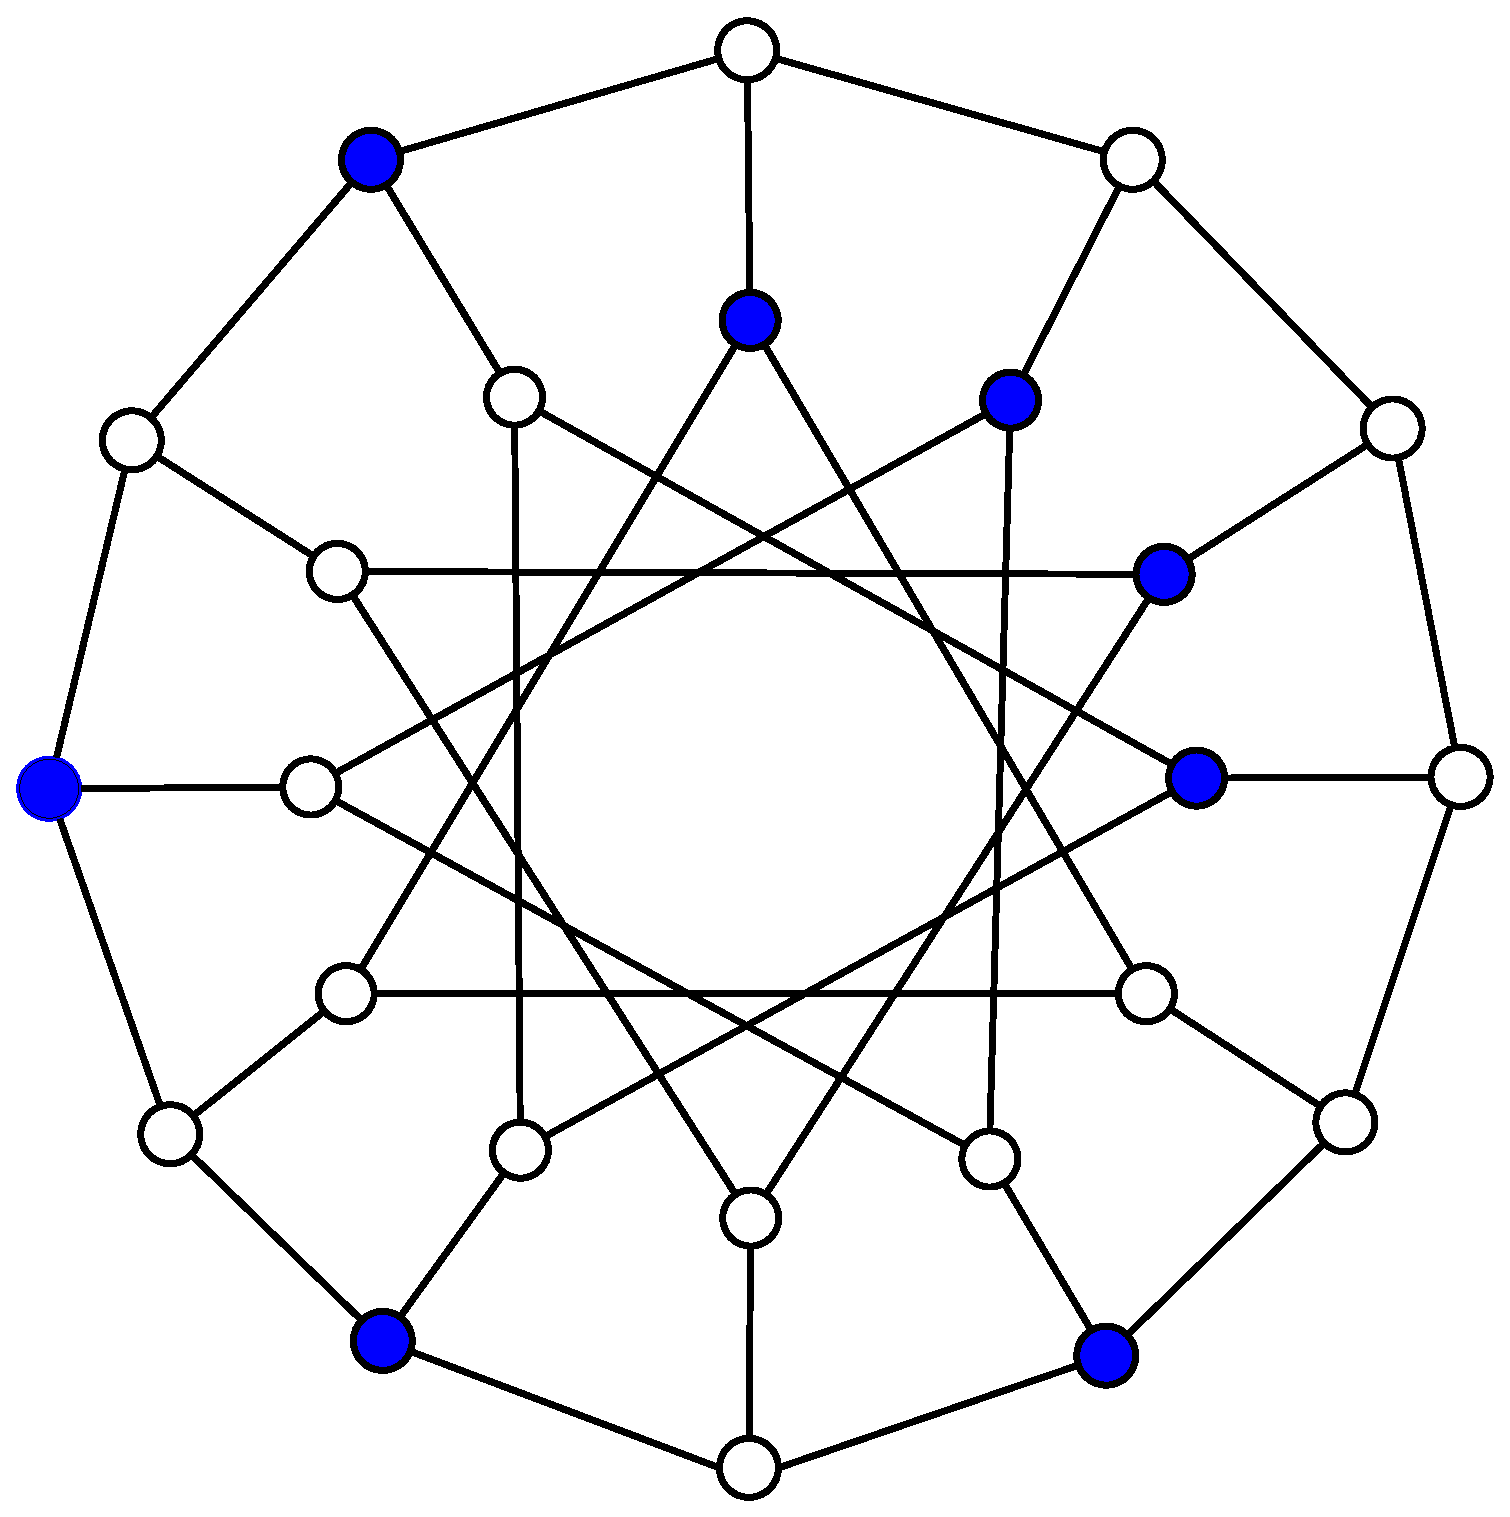
\includegraphics[width=\textwidth] {L3-independentsetgraph24-8.eps} 
 \end{minipage}
 \begin{minipage}{0.45\textwidth}
 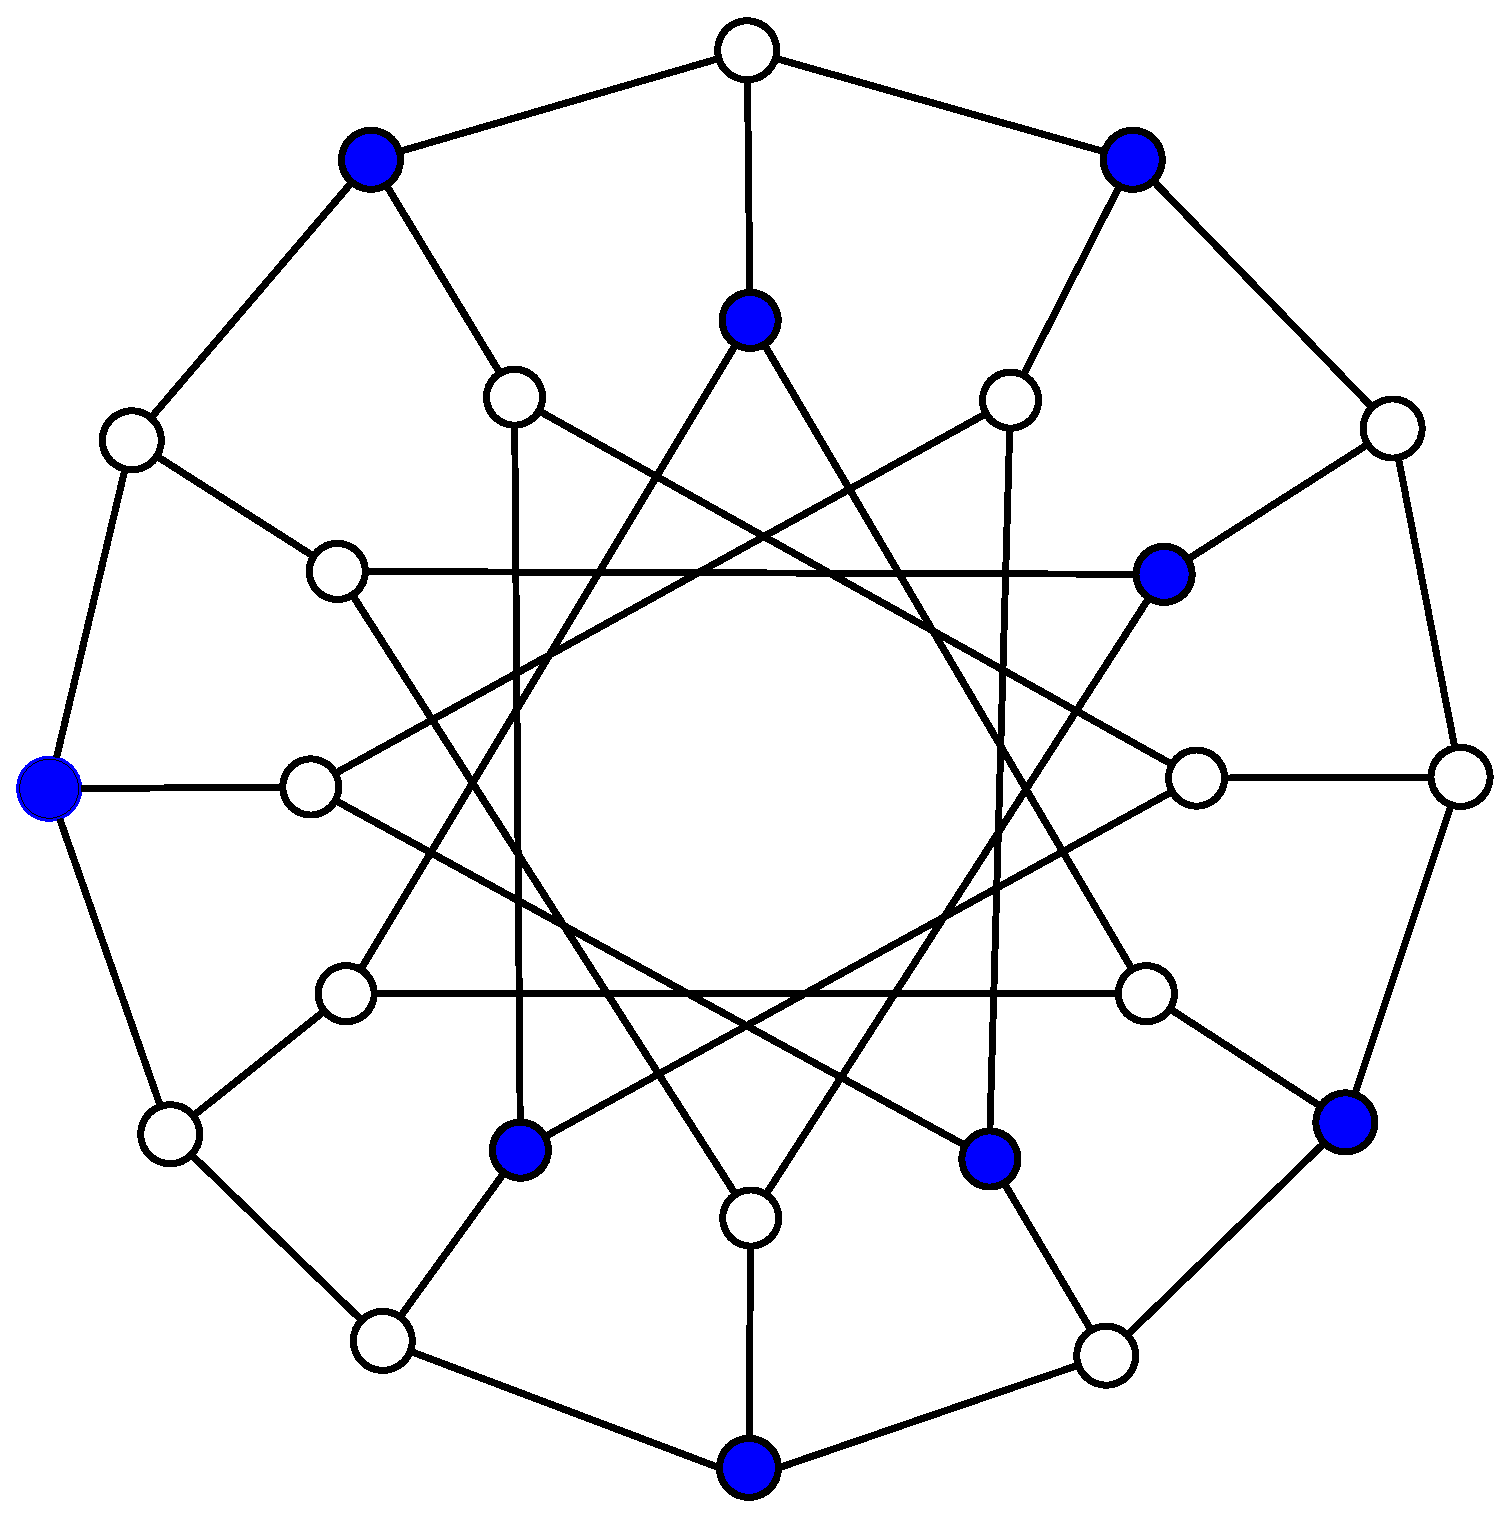
\includegraphics[width=\textwidth] {L3-independentsetgraph24-9.eps} 
\end{minipage}
\end{figure}
The nodes in blue form an independent set. Left: 8 nodes. Right: 9 nodes. 

}


\frame{
\frametitle{ {\sc Vertex Cover } Problem }

\begin{itemize}
 \item 
Practical problem: \\ {\em 
Given n sites connected with paths, how many guards (or cameras)  should be deployed on sites to surveille {\bf all} the paths?}

\begin{block}{Formalized Definition:}
 {\bf Input:} Given a graph $G=<V,E>$, and an integer $k$, \\
 {\bf Output:} is there a set of nodes $S  \subseteq V$, $|S| = k$, such that each edge has at least one of its endpoints in $S$? 
\end{block}

\item An example: are there 4 nodes to cover all edges in the following graph? 

\begin{figure}
\begin{tikzpicture}[scale=1.1, auto,swap]
    % Draw a 7,11 network
    % First we draw the vertices
    \foreach \pos/\name in {{(0,2)/v1}, {(2,2)/v2}, {(1,1)/v3}, {(2,1)/v4}, {(3,1)/v5}, {(0,0)/v6}, {(2,0)/v7}}
        \node[smallvertex] (\name) at \pos {};
        
    % Connect vertices with edges and draw weights
    \foreach \source/ \dest /\weight in {v1/v2/{}, v1/v3/{}, v2/v3/{}, v2/v4/{}, v2/v5/{}, v3/v6/{}, v3/v7/{}, v6/v7/{}, v4/v7/{}, v5/v7/{}  }
        \path[undirectededge] (\source) -- node[weight] {$\weight$} (\dest);
%       \draw[dashed, ->] (0,0) arc  (120:60:2);

      \end{tikzpicture}

\end{figure}

\end{itemize} 

} 

\frame{
\frametitle{ An example } 

\begin{figure}
\begin{tikzpicture}[scale=1.1, auto,swap]
    % Draw a 7,11 network
    % First we draw the vertices
    \foreach \pos/\name in {{(0,2)/v1}, {(2,2)/v2}, {(1,1)/v3}, {(2,1)/v4}, {(3,1)/v5}, {(0,0)/v6}, {(2,0)/v7}}
        \node[smallvertex] (\name) at \pos {};
        
    % Connect vertices with edges and draw weights
    \foreach \source/ \dest /\weight in {v1/v2/{}, v1/v3/{}, v2/v3/{}, v2/v4/{}, v2/v5/{}, v3/v6/{}, v3/v7/{}, v6/v7/{}, v4/v7/{}, v5/v7/{}  }
        \path[undirectededge] (\source) -- node[weight] {$\weight$} (\dest);
%       \draw[dashed, ->] (0,0) arc  (120:60:2);

    \foreach \pos/\name in { {(1,1)/v3}, {(2,1)/v4}, {(3,1)/v5}}
        \node[blue smallvertex] (\name) at \pos {};

    \foreach \pos/\name in { {(0,2)/v1}, {(2,2)/v2},  {(0,0)/v6}, {(2,0)/v7}}
        \node[red smallvertex] (\name) at \pos {};
      \end{tikzpicture}

\end{figure}

\begin{itemize}
\item 
Observation: the complement of an independent set (in blue) forms a vertex cover (in red).
\end{itemize}
}


\frame{
\frametitle{Reduction: {\sc Independent Set} $\le_P$ {\sc Vertex Cover} }

\begin{itemize}
 \item 
\textcolor{blue}{\bf Transformation:} map an {\sc IndependentSet} instance $<G, k>$ to a {\sc VertexCover} instance $<G', k'>$, where $G'=G$, and $k'=n-k$; \\
\end{itemize}
\begin{figure}
 \centering
 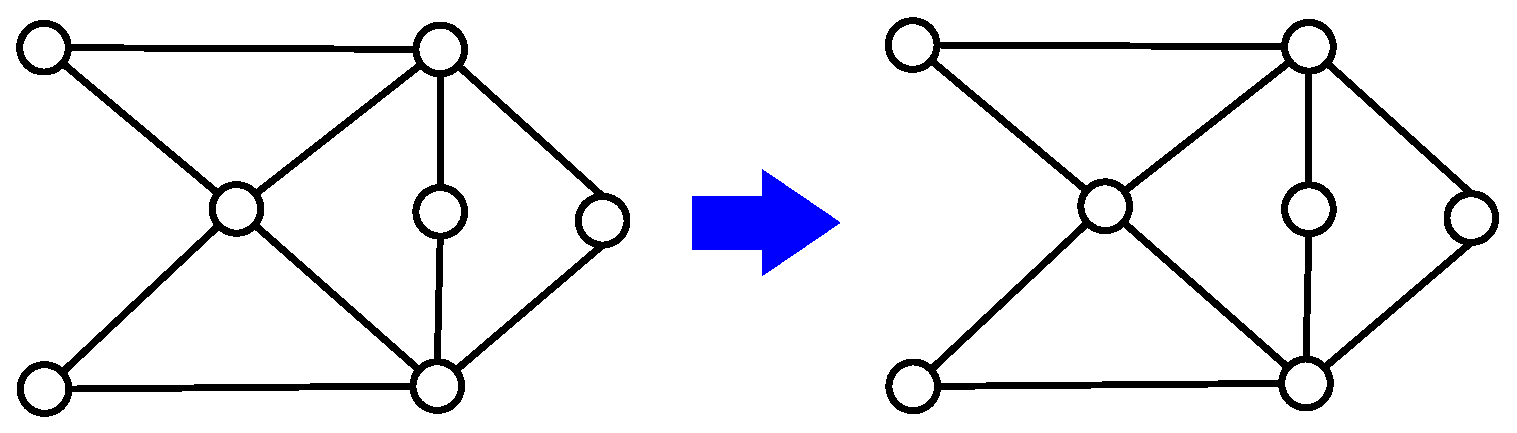
\includegraphics[width=3in]{L3-independentsettovertexcover.eps}
 \caption{Transformation from an {\sc Independent Set} instance $(G, k=3)$ into a {\sc Vertex Cover} instance $(G'=G, k'=4)$}
\end{figure}

} 

\frame{
\frametitle{Reduction: {\sc Independent Set} $\le_P$ {\sc Vertex Cover} }



\begin{Theorem}
\textcolor{blue}{\bf Equivalence:} $G$ has an independent set $S$ ($|S|=k$) $\Leftrightarrow$ $G'$ has a vertex cover $S'$ ($|S'|=n-k$). 
\end{Theorem} 


 
\begin{Proof}
\begin{itemize}
\begin{small}
 \item Let $S$ be an independent set of $G$ (in blue);\\
 \item For an arbitrary edge $e=(u,v)$, we have $u \not\in S$ or $v \not\in S$; 
 \item Thus, $u \in V-S$ or $v \in V-S$;
 \item Define $S'=V-S$ (in red). $S'$ is a vertex cover of $G'=G$, and $|S'| = n-k$.
\end{small}
\end{itemize}
\end{Proof}

\begin{figure}
 \centering
 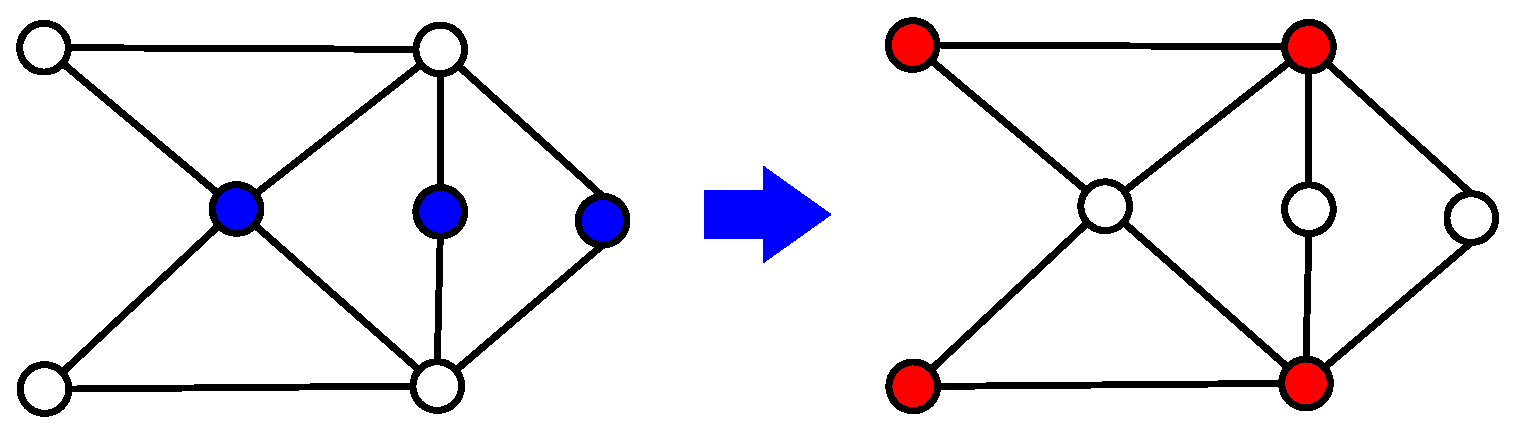
\includegraphics[width=2.4in]{L3-independentsettovertexcoverredblue.eps}
 \caption{ {\small The complement of an  independent set(in blue) form a vertex cover (in red)} } 
 \end{figure}
 
}

\frame{
\frametitle{How to do reduction?}
C. Papadimitriou said: 

{\it 
To show the problem NP-complete we start by toying with small instances of the problem, 

until we isolate one with an interesting behavior. 

Sometimes the properties of this instance immediately enable a simple NP-complete proof .... sometimes called ``gadget construction''...
}

(Excerpted from Computer and Complexity)
}


\frame{
\frametitle{}
\begin{block}{}
 Another simple reduction: {\sc Vertex Cover} $\le_P$ {\sc Set Cover}.
\end{block}
}

\frame{
\frametitle{ {\sc Set Cover} problem}
\begin{itemize}
 \item 
Practical problem: \\ {\em  
An anti-virus package identifies a virus based on its characteristic ``keywords'' set. A keyword might correspond to several viruses. To reduce the size of anti-virus software, it is interesting to detect  all viruses using a set of ``representative'' keywords rather than all keywords. }


\begin{block}{Formalized Definition: } 
{\bf Input:} a set $U$ of $n$ elements, a collection $S_1, S_2,...,S_m$ of subsets of $U$, and a number $k$. \\
{\bf Output:}  does there exist a collection of at most $k$ of these sets whose union is equal to $U$?
\end{block}
\end{itemize}

}

\frame{
\frametitle{ {\sc Set Cover} problem: an interesting instance}

\begin{figure}
 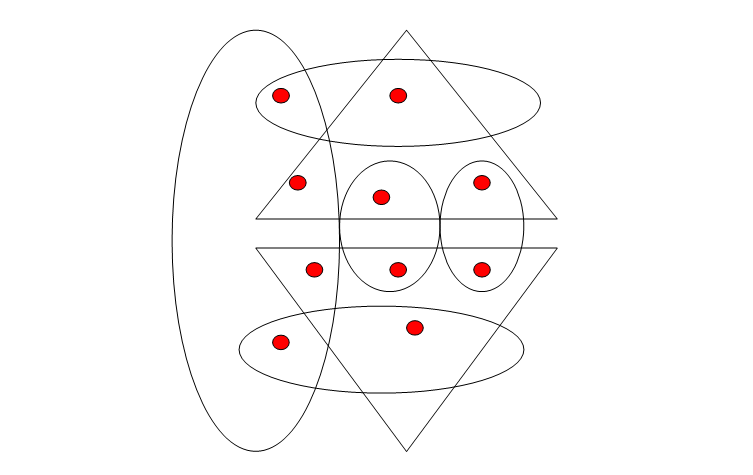
\includegraphics[width=2in]{setcover1.png}
 % setcover1.eps: 22002048x0 pixel, 300 dpi, 186284.00x0.00 cm, bb=14 14 407 318
\end{figure}
In this instance, there is a collection of three of the sets whose union is equal to all of $U$: We can choose the tall thin oval on the left, together with the two polygons.
}


\frame{
\frametitle{Reduction: {\sc Vertex Cover} $\le_P$ {\sc Set Cover}}

\begin{itemize}
 \item 

Key observation: a special case of {\sc Set Cover}, where each element is covered by exactly two subsets, is in fact {\sc Vertex Cover}.
\begin{enumerate}
 \item 
Transformation: Given a {\sc Vertex Cover} instance $<G, k>$, create a {\sc Set Cover} instance: $k'=k$, $U=E$, $S_v = \{$ e : e incident to v$\}$; \\

%\begin{figure}
% 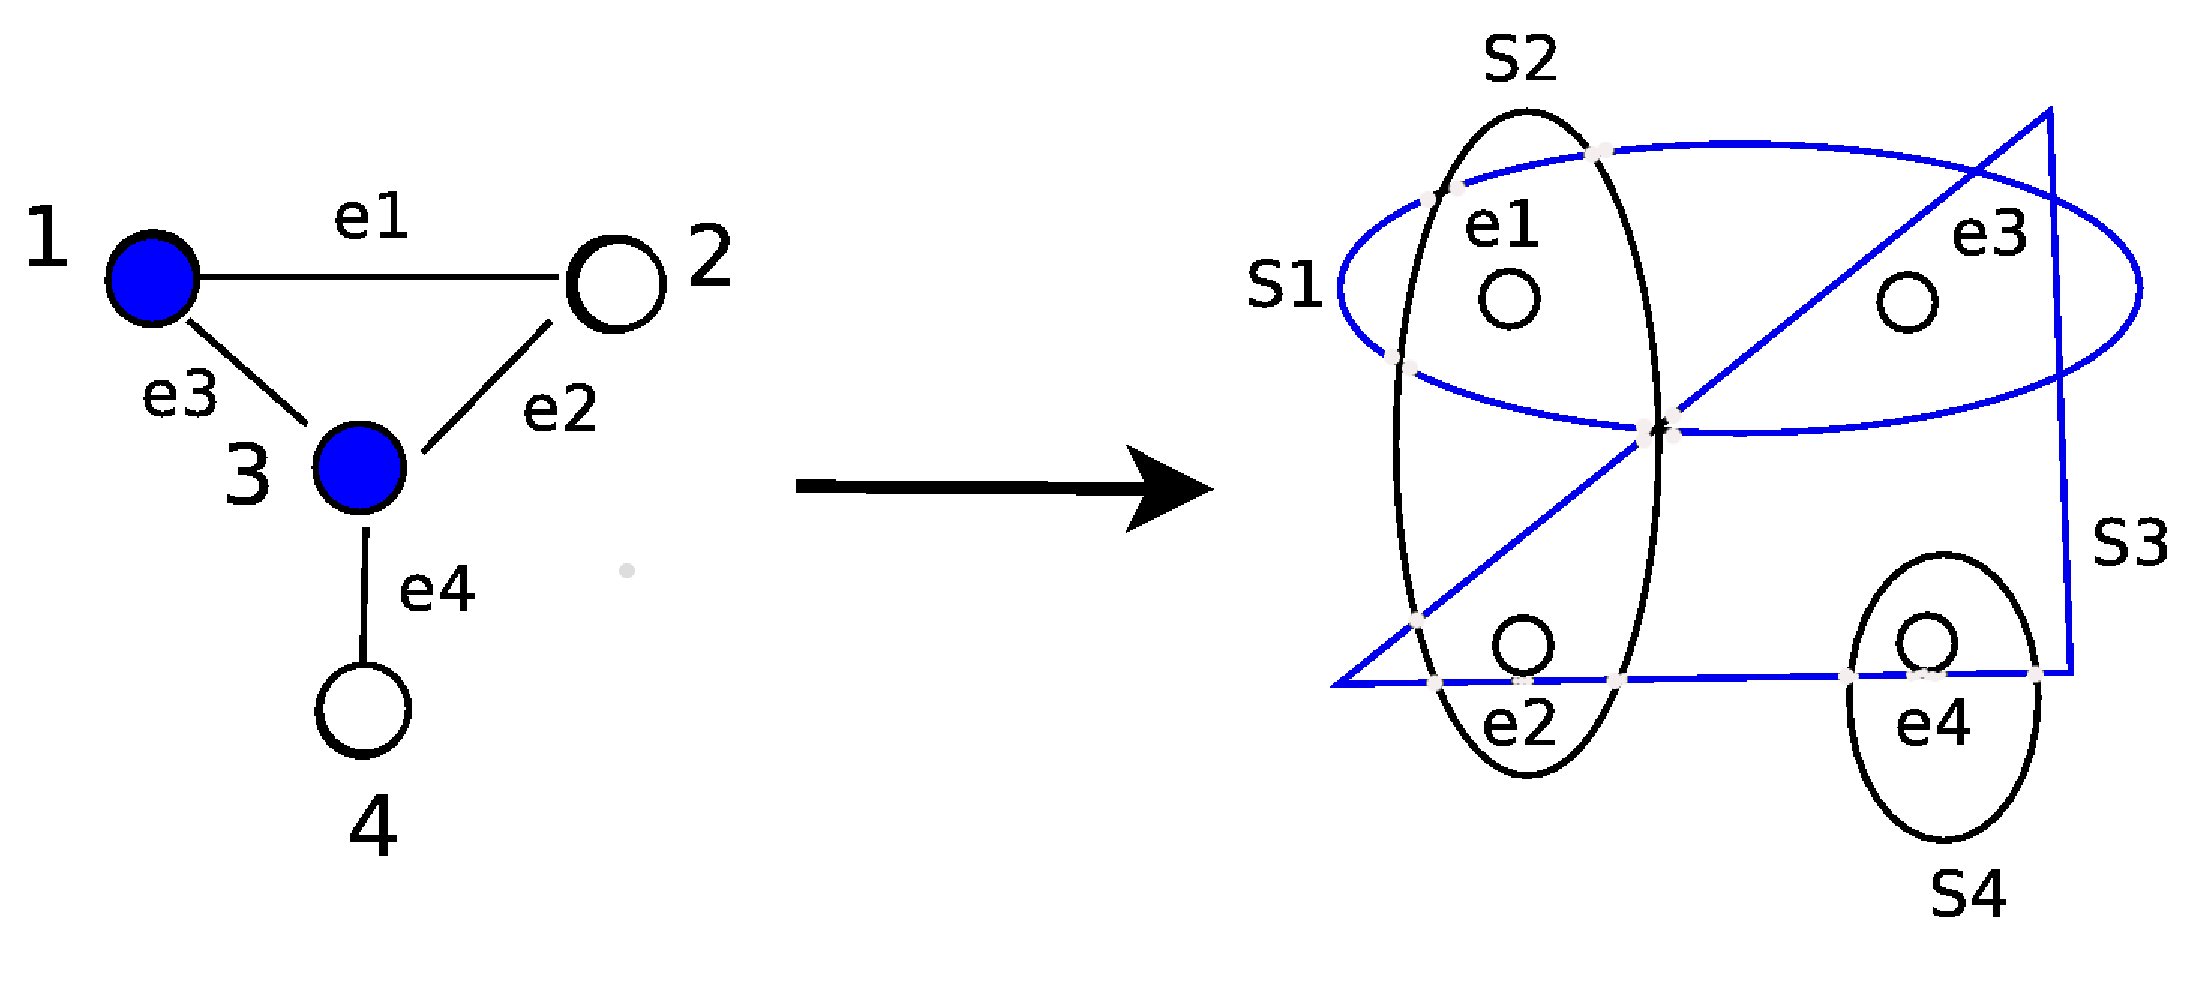
\includegraphics[width=2.8in]{L3-vertexcoversetcover.eps}
% % setcover1.eps: 22002048x0 pixel, 300 dpi, 186284.00x0.00 cm, bb=14 14 407 318
%\end{figure}
\begin{figure}[H]
	\center
	\begin{tikzpicture}[scale=1.3, auto,swap]
	\path  (-1.5,0)  coordinate(O);
	\path  (0,0)  coordinate(A);
	\path[edge,blue] (O)--(A);
	
	\draw (2,0) ellipse (0.4cm and 1.6cm);
	\draw (3,1)ellipse (1.6cm and 0.4cm);
	
	\path (4.2,1.4) coordinate (A);
	\path (1.5,-1.2) coordinate (B);
	\path (4.2,-1.2) coordinate (C);
	\draw (A) -- (B) -- (C) -- cycle;
	\foreach \pos/\name in {{(-4,1)/1},{(-3,0)/3}}
	\node[smallvertex, draw,fill=blue]  (\name)at \pos{};
	\node[ultra thick, left,black] at (1.west) {1};
	\node[ultra thick, left,black] at (3.west) {3};
	\foreach \pos/\name in {{(-2,1)/2},{(-3,-1)/4}}
	\node[smallvertex, draw,fill=white]  (\name)at \pos{};  
	\node[ultra thick, right,black] at (2.east) {2};
	\node[ultra thick, below,black] at (4.south) {4};
	\foreach \source/ \dest /\weight in {1/2/{e1}, 2/3/{e2},1/3/{e3},3/4/{e4}}
	\draw[sloped, midway, below] (\source) -- node[weight] {$\weight$} (\dest);
	
	\foreach \pos/\name in {{(2,1)/e1},{(4,1)/e3},{(2,-1)/e2},{(4,-1)/e4}}
	\node[smallvertex, draw,fill=white]  (\name)at \pos{};
	\node[ultra thick, above,black] at (e1.north) {e1};
	\node[ultra thick, below,black] at (e2.south) {e2};      
	\node[ultra thick, above,black] at (e3.north) {e3};
	\node[ultra thick, below,black] at (e4.south) {e4};          
	\end{tikzpicture}
\end{figure}

\item 
Equivalence: $G$ has a vertex cover $C$ ($|C|=k$) (in blue) $ \Leftrightarrow$ $S_c$ ($c\in C$) describe a set cover (in blue).
\end{enumerate}
\end{itemize}

}

\frame{
\frametitle{}
\begin{block}{}
 A reduction via ``Gadget'': {\sc 3-SAT} $\le_P$ {\sc Independent Set}.
\end{block}
}

\frame{
\frametitle{ {\sc SAT (Satisfiability)} Problem }
\begin{itemize} 
\item Practical problems:  \\ {\em 
      expressing constraints on a set of variables (in AI), verifying whether a circuit has the desired functionality (in VLSI), etc. } 
  
\begin{block}{Formalized Definition:} 
 {\bf Input:} Given a CNF $\phi = C_1 \wedge C_2 ... \wedge C_k$; \\
{\bf Output:} Is there an assignment of all $x_i$ such that all clauses $C_j$ are satisfied? 
\end{block}
 \item Notations: 
\begin{itemize}
 \item Boolean variable: $x_1, x_2, ..., x_n$, $x_i = \texttt{TRUE/FALSE} $;
 \item Literal (or term): a variable $x_i$, or its negative $\neg x_i$;
 \item Clause: a disjunction of literals: $C_1 = x_1 \vee \neg x_2 \vee ... \vee x_3 $;
 \item CNF( Conjunctive normal form): the conjunctions of clauses; $\phi = C_1 \wedge C_2 ... \wedge C_k$;
\end{itemize}
\item 
Example: 
\begin{itemize}
\item CNF:  $(x_1 \vee \neg x_2) \wedge ( \neg x_1 \vee \neg x_3 ) \wedge ( x_2 \vee \neg x_3 )$
\item 
\texttt{TRUE} assignment:  $x_1 = \texttt{FALSE}, x_2= \texttt{FALSE}, x_3 = \texttt{FALSE} $;
\end{itemize}
\end{itemize}

}

\frame{
\frametitle{ {\sc SAT (Satisfiability)} Problem: Two viewpoints of \texttt{TRUE}  assignment }
\begin{itemize}
 
\item 
Example: 
\begin{itemize}
\item CNF:  $(x_1 \vee \neg x_2) \wedge ( \neg x_1 \vee \neg x_3 ) \wedge ( x_2 \vee \neg x_3 )$
\item 
True assignment:  $x_1 = \texttt{FALSE}, x_2= \texttt{FALSE}, x_3 = \texttt{FALSE} $;
\end{itemize}
\item 
Two viewpoints of a $\texttt{TRUE}$ assignment:
\begin{enumerate}
 \item Variables: giving each variable a $\texttt{TRUE/FALSE}$ to satisfy all clauses;
 \item Clauses: In each clause, we select a literal and set it to be $\texttt{TRUE}$  to make the clause satisfied. However, there should be no conflict among the  selected literals from different clauses, e.g., select $x_i$ from one clause and select $\neg x_i$ from another one. 
\end{enumerate}
\end{itemize}
}


\frame{
\frametitle{{\sc Independent Set}: designing gadget }

\begin{itemize}
 \item \textcolor{red}{\bf Gadget}: a small, useful, and cleverly-designed machine or tool; a piece with specific functionality, which can be used to simulate another problem, say, to simulate \textcolor{red}{\bf variables}  and \textcolor{red}{\bf clauses} in SAT problem.
 
\item For example, in {\sc Independent Set} problem, clique is a gadget with functionality \textcolor{red}{\bf OR}. Consider the three nodes in the following {\sc Independent Set} instance: 
 
 \begin{figure}
 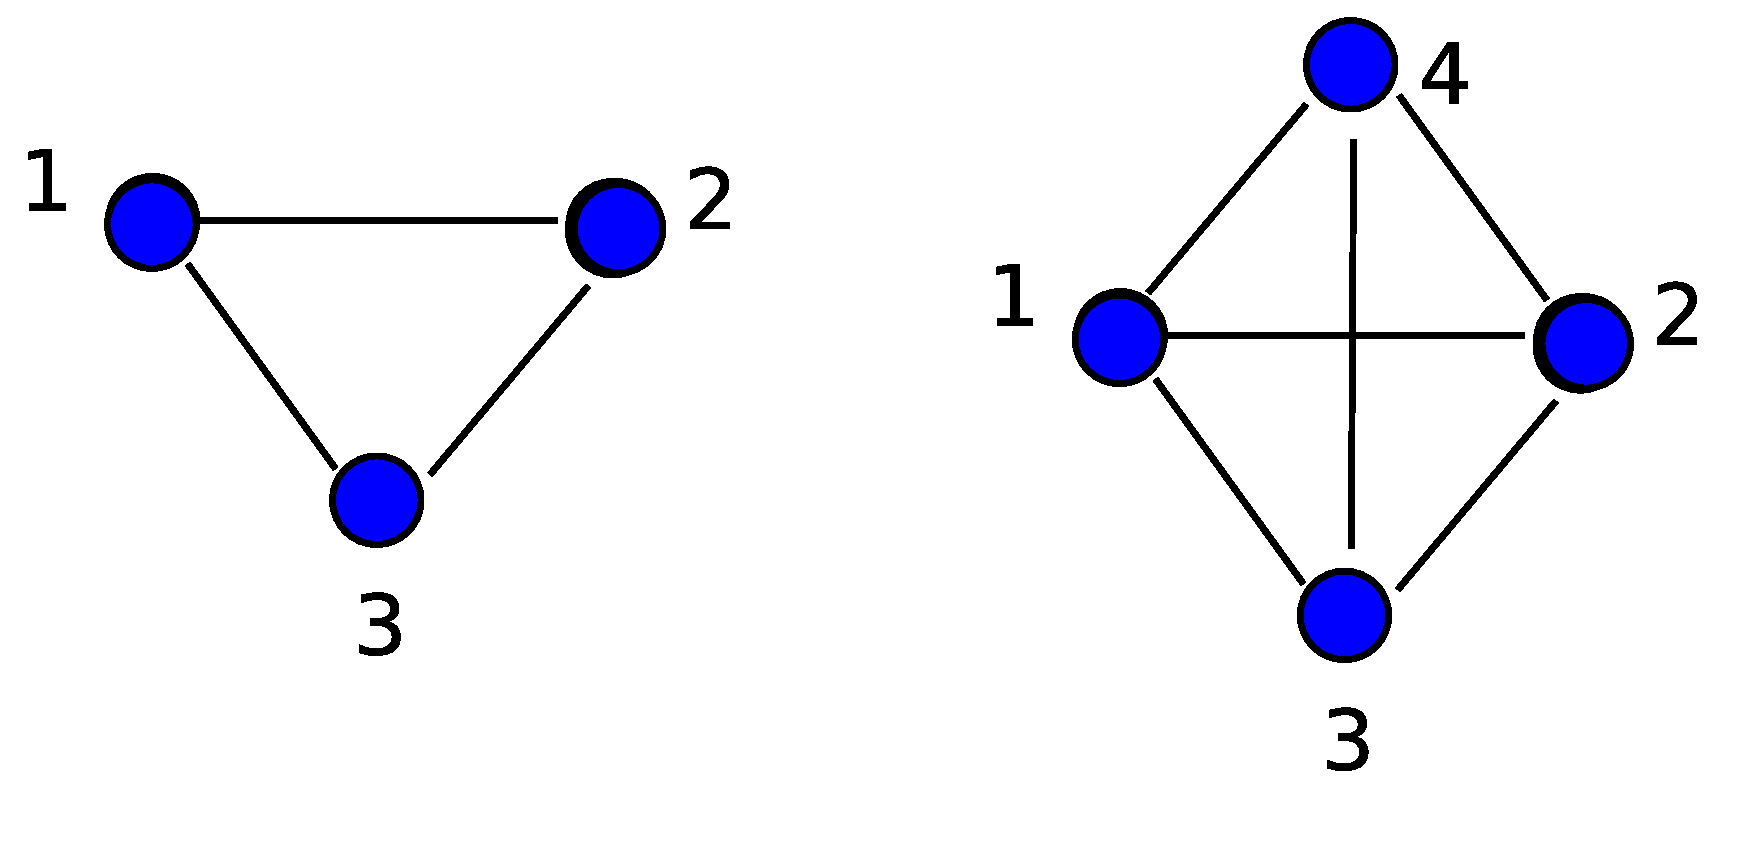
\includegraphics[width=1.9in]{L3-clique.eps}
\end{figure}

\item 
We can 
\textcolor{red}{\bf choose 1 OR choose 2 OR choose 3}  since only one vertex of a clique can appear in an independent set. 

\item 
Thus, we can use it to simulate the \textcolor{red}{\bf OR} operator in a clause. 
\end{itemize}
}

%\frame{
%\frametitle{How does a gadget work? }
%
%\begin{itemize}
%\item Consider the following {\sc Independent Set} instance: 
%\begin{figure}
% 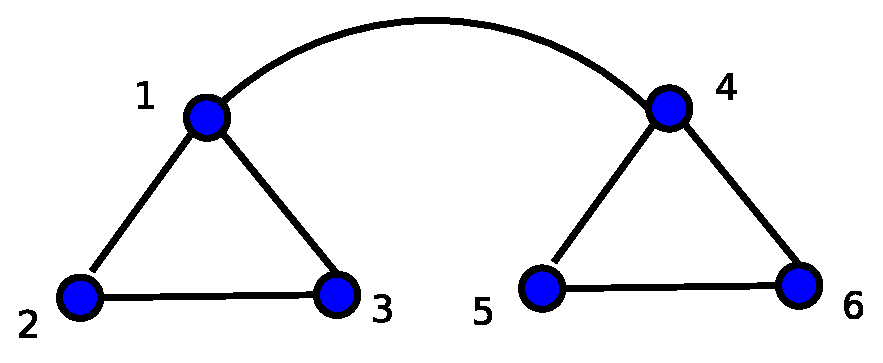
\includegraphics[width=1.9in]{L3-independentsetsat.eps}
%\end{figure}
%
%\item Let's denote the selection of node $i$ as $x_i = \texttt{TRUE}$. Then we have: 
%\begin{enumerate} 
% \item We cannot choose 1 AND 4 simultaneously; (variable: $x_1 = \neg x_4$ ) 
% \item We can choose 1 OR 2 OR 3;          (clause:  $C_1 = x_1 \vee x_2 \vee x_3 $)
% \item We can choose 4 OR 5 OR 6;	   (clause: $C_2 = \neg x_1 \vee x_5 \vee x_6 $)	
%\end{enumerate}
% \item Suppose we were required to select an independent set of 2 vertices, we have to choose one vertex from 1,2,3 AND another vertex from 4,5,6.  	( CNF:  $\Phi = C_1 \wedge C_2$ )
% %\item $( x_1 \vee x_2 \vee x_3 ) \wedge ( \neg x_1 \vee x_5 \vee x_6)$. ($x_i$ means the selection of node $i$ in {\sc Independent Set}. )
%\end{itemize}
%}

\frame{
\frametitle{{\sc 3SAT} $\le_P$ {\sc Independent Set}: Transformation }

\begin{itemize}
 \item 
\textcolor{blue}{\bf Transformation:} 
 
\begin{itemize}
 \item 
   For a given $SAT$ instance $\phi$ with $k$ clauses, constructing an {\sc Independent Set} instance $(G, k')$ as follows: 
\begin{enumerate}
 \item $G$ consists of $k$ triangles: each triangle corresponds to a clause $C_i$; the nodes are labeled with the literals; connecting $x_i$ and $\neg x_i$ with an edge; \\

 \item Set $k' = k$; 
\end{enumerate}
\item 
Example: 

\begin{figure}
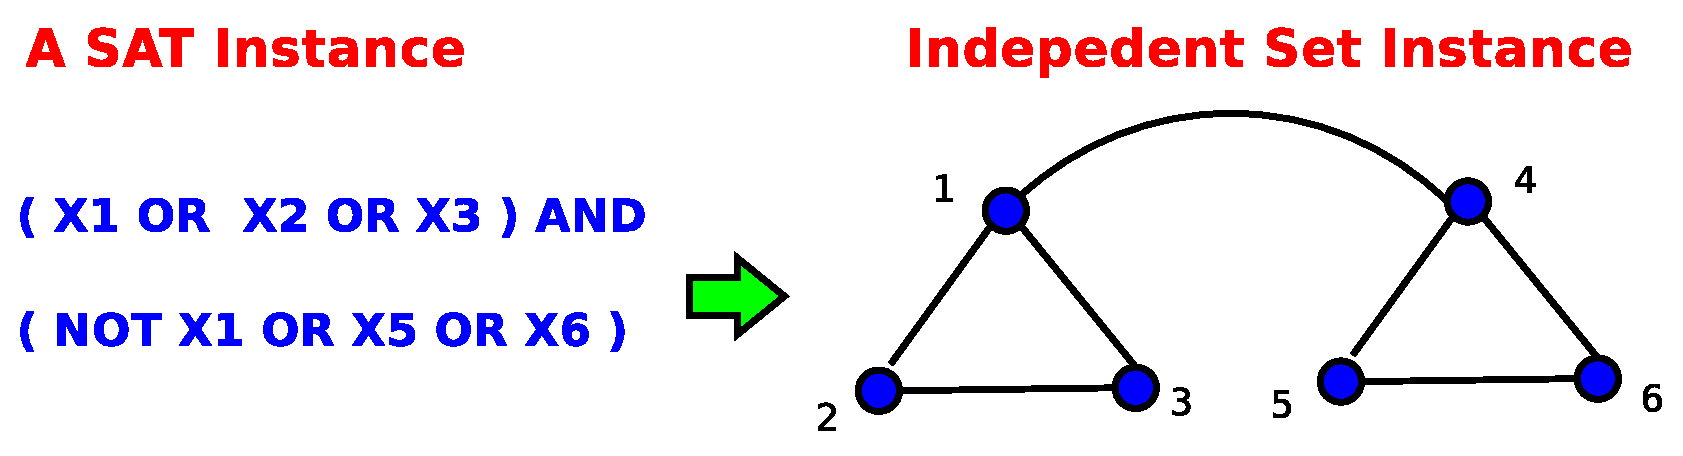
\includegraphics[width=3in]{L3-satindependentset.eps}
\end{figure}

\item 
Intuition: edge represents ``conflicts''; we should identify $k$ nodes (each node from a triangle) without connections (no conflict);
\end{itemize}
\end{itemize}
}

\frame{
\frametitle{{\sc 3SAT} $\le_P$ {\sc Independent Set} }

\begin{itemize}
\item \textcolor{blue}{\bf Equivalence: }

\begin{figure}
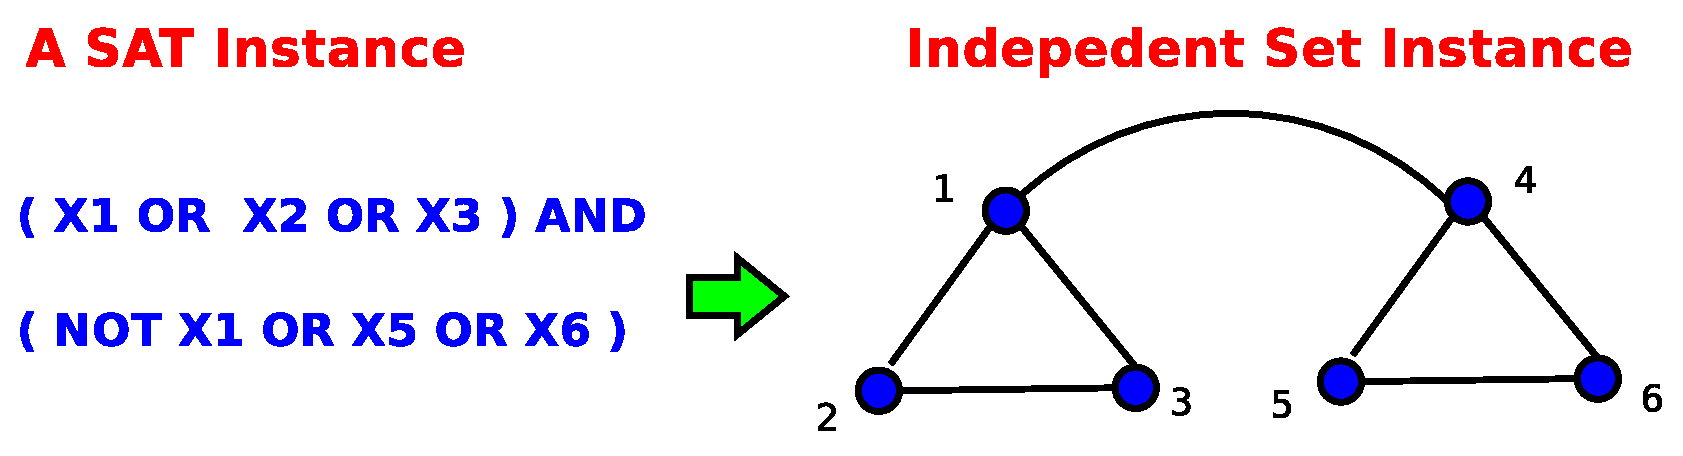
\includegraphics[width=3in]{L3-satindependentset.eps}
\end{figure}

\begin{Proof}
\begin{itemize}
 \item 
Suppose $\phi$ is satisfiable; \\
\item 
There is an assignment such that in each clause, at least one literal is satisfied;  \\
\item 
Choose exactly one satisfied literal from each clause;  \\
\item 
The corresponding nodes form an independent set;  
\end{itemize}
\end{Proof}
\end{itemize}

} 


\frame{
\frametitle{{\sc 3SAT} $\le_P$ {\sc Independent Set}: Equivalence }
\begin{itemize}
\item \textcolor{blue}{\bf Equivalence: }

\begin{figure}
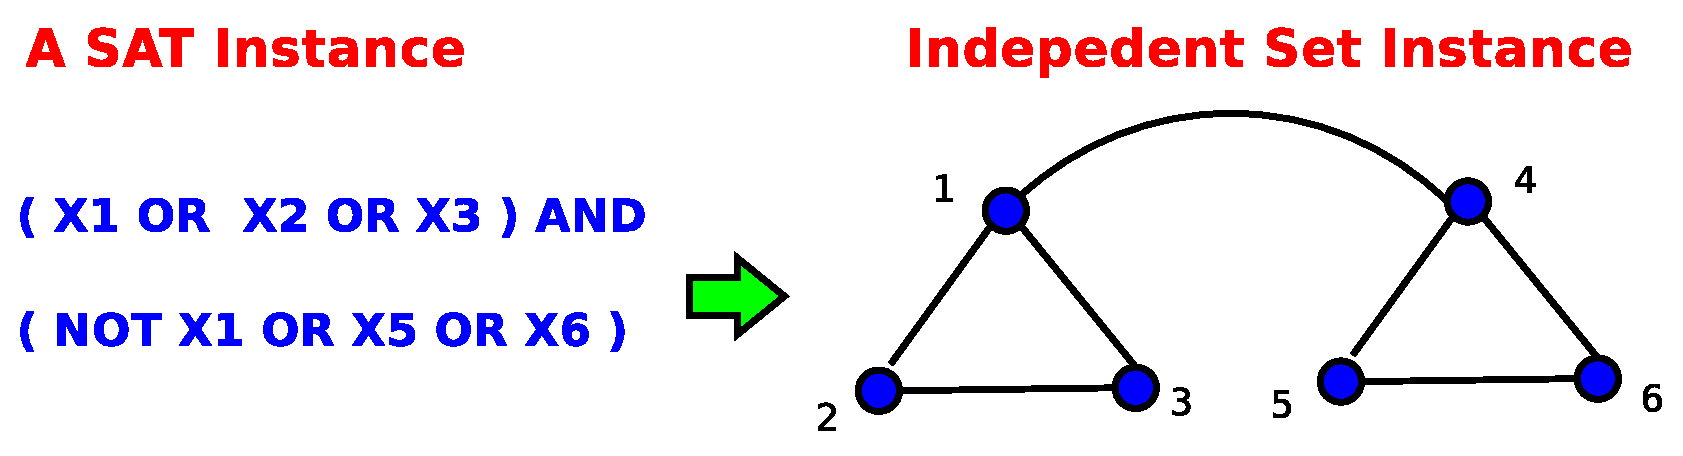
\includegraphics[width=3in]{L3-satindependentset.eps}
\end{figure}

\begin{Proof}
\begin{itemize}
 \item 
Suppose $S$ is an independent set, and $|S|=k$;  \\
\item 
$S$ contains exactly one node from each triangle; (?) \\
\item 
Constructing an assignment: if $v_i \in S$, $x_i=TRUE$, and  $x_i = FALSE$ otherwise; \\
\item 
Notice that $v_i$ and $\neg v_i$ would not appear in $S$ simultaneously. 
\item 
$\phi$ is satisfied by this assignment. 
\end{itemize}
\end{Proof}
\end{itemize}
}

\frame{
\frametitle{}
\begin{block}{}
 Another reduction via ``gadget'': {\sc SAT } $\le_P$ {\sc Hamilton Cycle}.
\end{block}
}


\frame{
\frametitle{ {\sc Hamilton Cycle} Problem}

\begin{figure}
  \subfigure{ 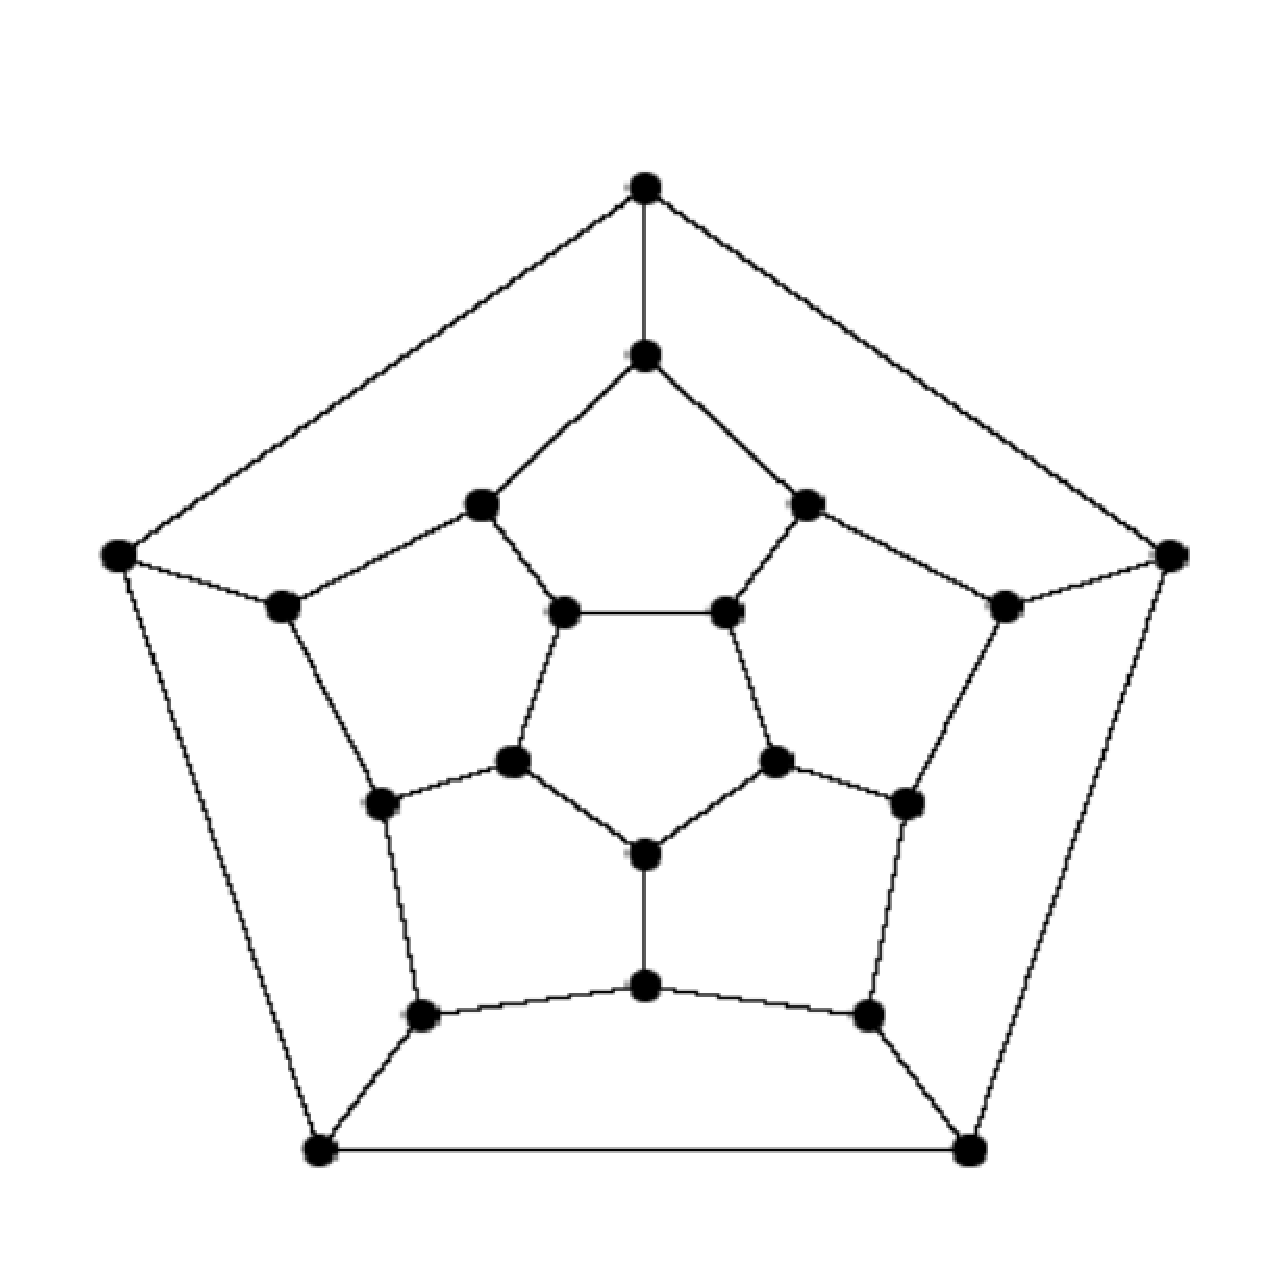
\includegraphics[height=1.3in]{L3-hamiltoncyclegame.eps} } 
  \subfigure{ 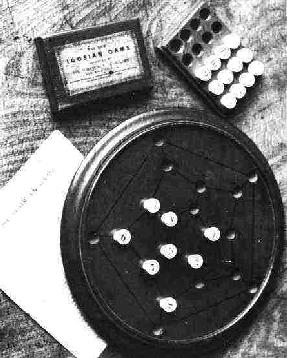
\includegraphics[height=1.3in]{L3-hamiltoncyclegameboard.png} } 
\end{figure}

A game invented by Sir William Hamilton in 1857. 

\begin{block}{Formalized Definition:}
 {\bf Input:} Given a graph $G=<V,E>$ \\
 {\bf Output:} Is there a cycle visiting every node exactly once?
\end{block}
}

\frame{ 
\frametitle{{\sc Hamilton Cycle}: two examples  } 
\begin{figure}
  \subfigure{ 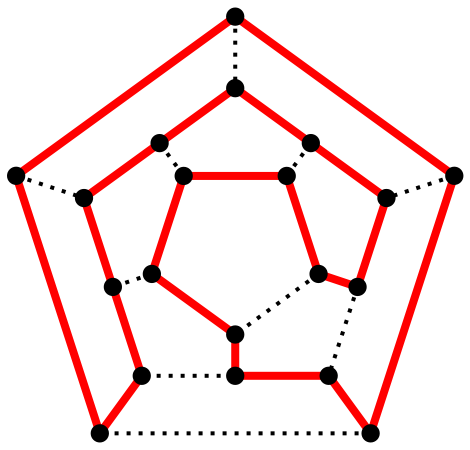
\includegraphics[height=1.5in]{L3-hamiltoncycleexample1.png} } 
  \subfigure{ 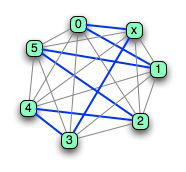
\includegraphics[height=1.5in]{L3-hamiltoncycleexample2.png} } 
\end{figure}
} 


\frame{
\frametitle{DNA sequencing: an application of {\sc Hamiltonian Cycle}}

\begin{figure}
 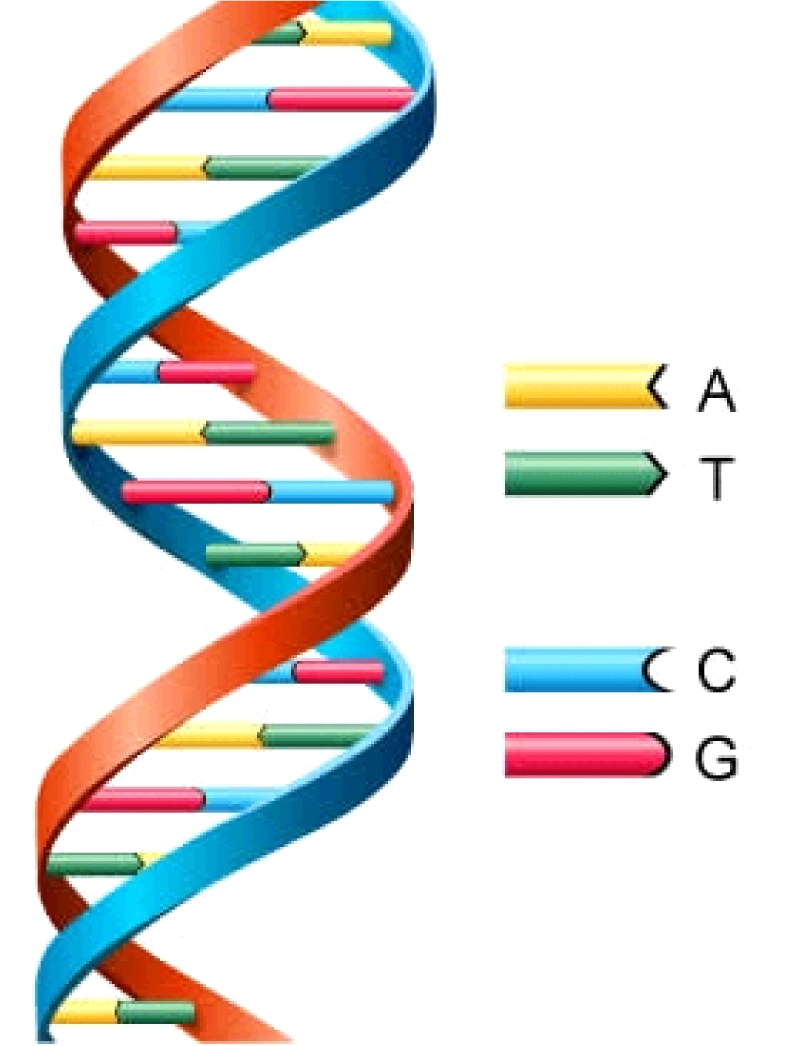
\includegraphics[width=0.5in]{L3-DNA.png}
\end{figure}
\begin{figure}
 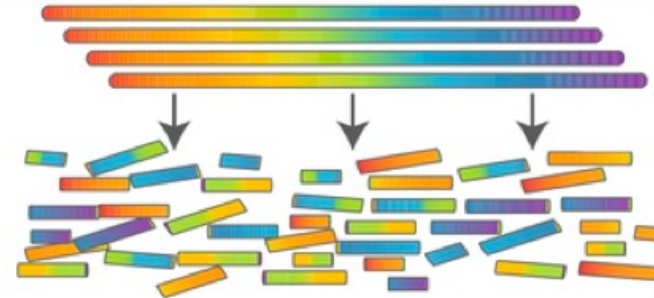
\includegraphics[width=2in]{L3-dnasequencing.png}
\end{figure}

\begin{itemize}
\item  
Multiple copies of a DNA $\Rightarrow$ small sequenced fragments called reads (say ~500 bp). 
\item Challenge: how to restore the whole genome from the short fragments? 
\end{itemize} 
\begin{footnotesize}
(see http://www.learner.org/courses/mathilluminated/interactives/dna/ for an animation)
\end{footnotesize}

}

%\frame{
%\frametitle{{\sc Hamilton Cycle} Application: DNA sequencing}
%
%\begin{small} 
%\begin{itemize}
% \item Intuition: 100 copies of a book were sheared (randomly) into scrips. Can we read out the book from these scrips?
% \item \textcolor{red}{Utilizing the overlapping information between two fragments to do fragment assembly! } 
% \item Construct a graph: a node denotes a fragment, and if the head of one fragment is equal to the tail of another fragment, we define a directed edge between the two fragments. 
% \item Observation: Reading the original sequence corresponds to traveling all nodes exactly once; thus we obtain a Hamilton path! \footnote{This is just an ideal case. In practice, the {\it repeats} in genome make things difficult: some nodes should be visited multiple times.}
%\end{itemize}
%\end{small}
%\begin{figure}
% 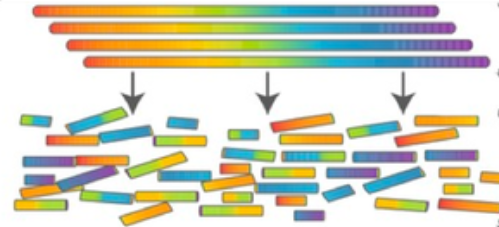
\includegraphics[width=4in]{L3-hamiltonpathdnanew.eps}
%\end{figure}
%}

\frame{
\frametitle{{\sc Hamiltonian Cycle} and genome assembly}

\begin{figure}
 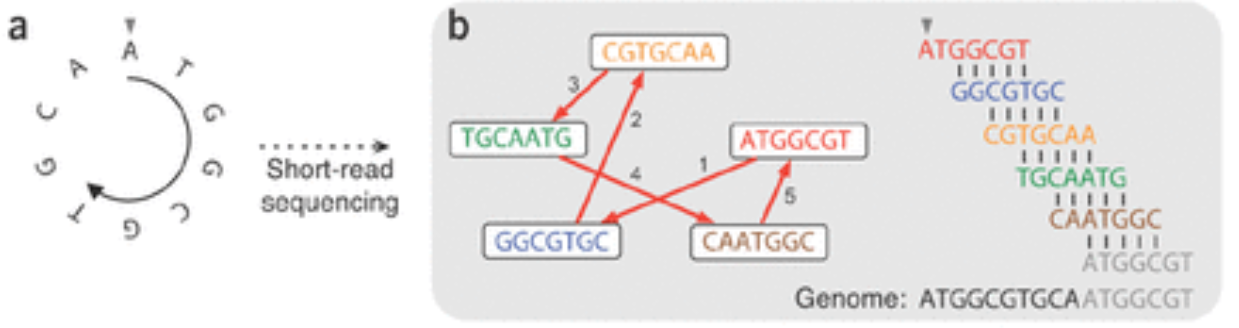
\includegraphics[width=4in]{L3-GenomeAssembly.png}
\end{figure}
\begin{itemize}
\item Let's construct a graph as follows: 
	\begin{itemize}
	\item node: a short fragment
	\item edge: if two fragments overlap, then an edge is added between the corresponding nodes; 
\end{itemize} 
\item Observation: {\sc Hamiltonian cycle} $\Leftrightarrow$ the genome 
\end{itemize} 
}


\frame{
\frametitle{{\sc Hamilton Cycle} problem:  designing gadget}

\begin{itemize}
\item Consider the following graph: 

\begin{figure}
 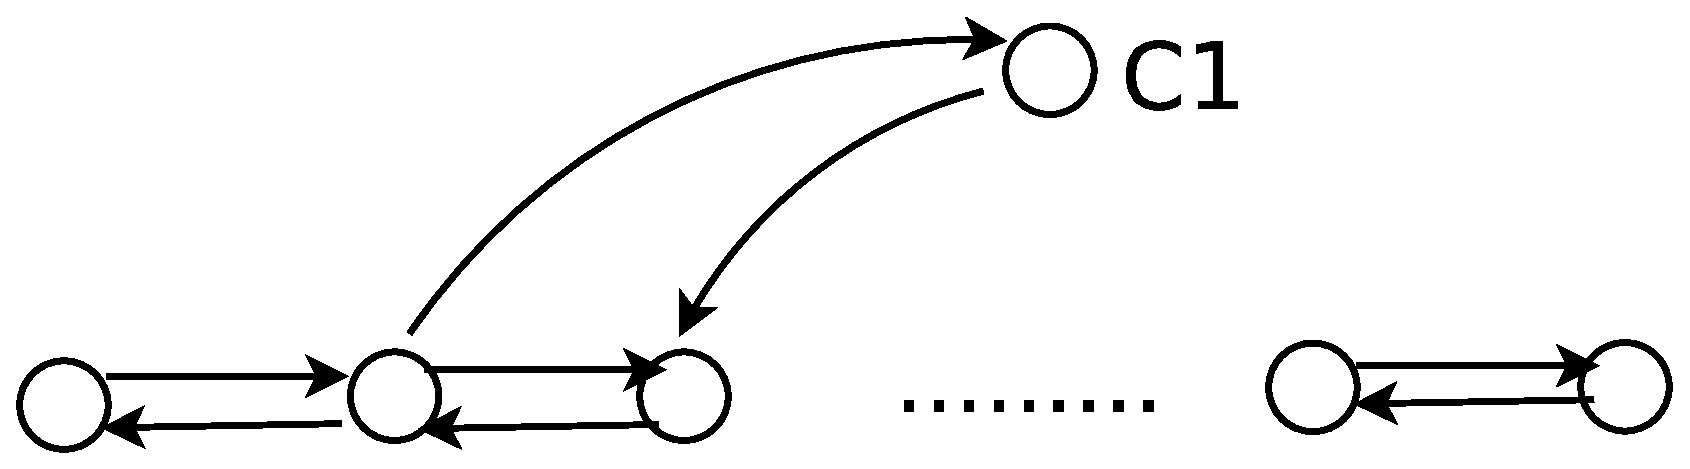
\includegraphics[width=2in]{L3-sathamiltongadgetsnocolor.eps}
\end{figure}

\item Suppose that we were required to visit all nodes. It is obvious that: 
\begin{itemize}
 \item To visit all nodes in the line, we can visit from left to right, \textcolor{red}{\bf OR} from right to left.  
 \item  However, in order to visit node $C_i$, the connection manner of $C_i$ defines the possible traveling direction of the line of nodes. For example, if we want to visit node $C_1$, we have to travel the line $P_1$ from left to right, or travel $P_2$ from right to left. 
 \begin{figure}
 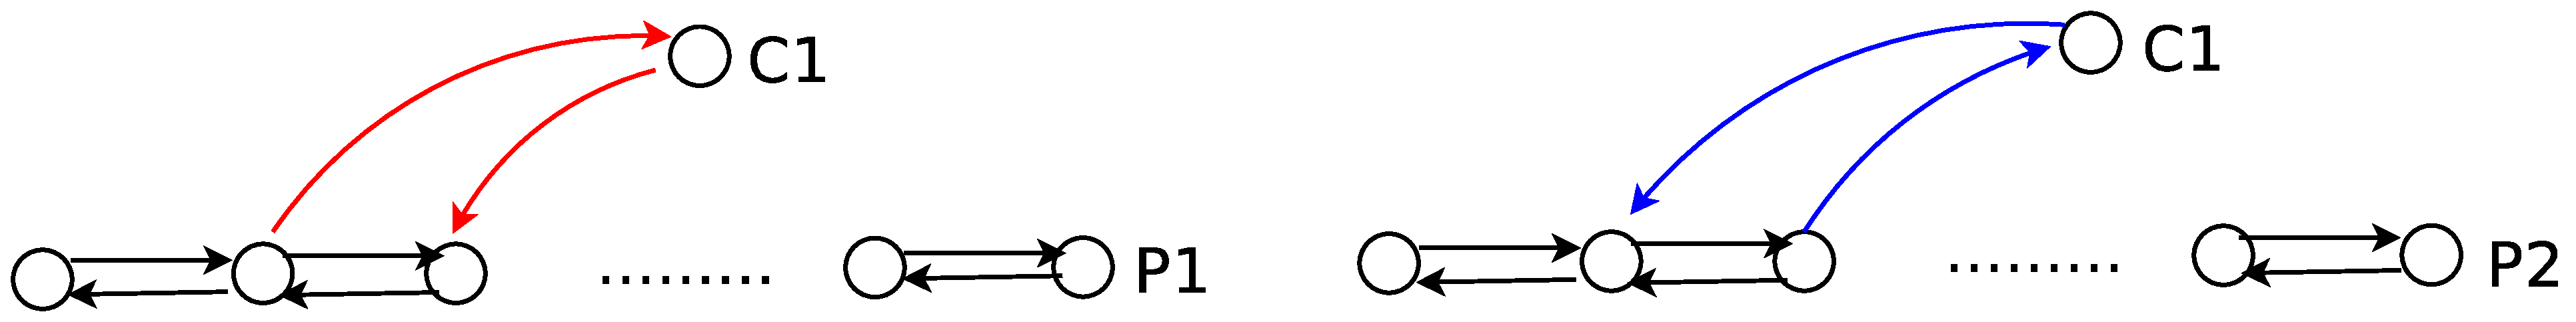
\includegraphics[width=4.0in]{L3-sathamiltongadgets.eps}
\end{figure}
\end{itemize}
\end{itemize}
}

\frame{
\frametitle{Reduction {\sc 3SAT} $\le_P$ {\sc Hamilton Cycle} } 

\begin{itemize}
\item 
\textcolor{blue}{\bf Transformation: }
\begin{itemize}
\item 
For a given SAT instance $\phi$, we construct a {\sc Hamilton Cycle} instance $G$ as follows: 

\begin{enumerate}
 \item 
 Variable $\Rightarrow$  a line of nodes for each variable; 
\item 
Clause $\Rightarrow$ a special node $C_i$. $C_i$ connects to the line $j$ in ``clockwise'' direction if it contains $x_j$ and connects in ``counter-clockwise'' direction if it contains $\neg x_j$. 
\item Two special nodes $s$ and $t$: 
\end{enumerate}
\end{itemize}
\end{itemize}
\begin{figure}
 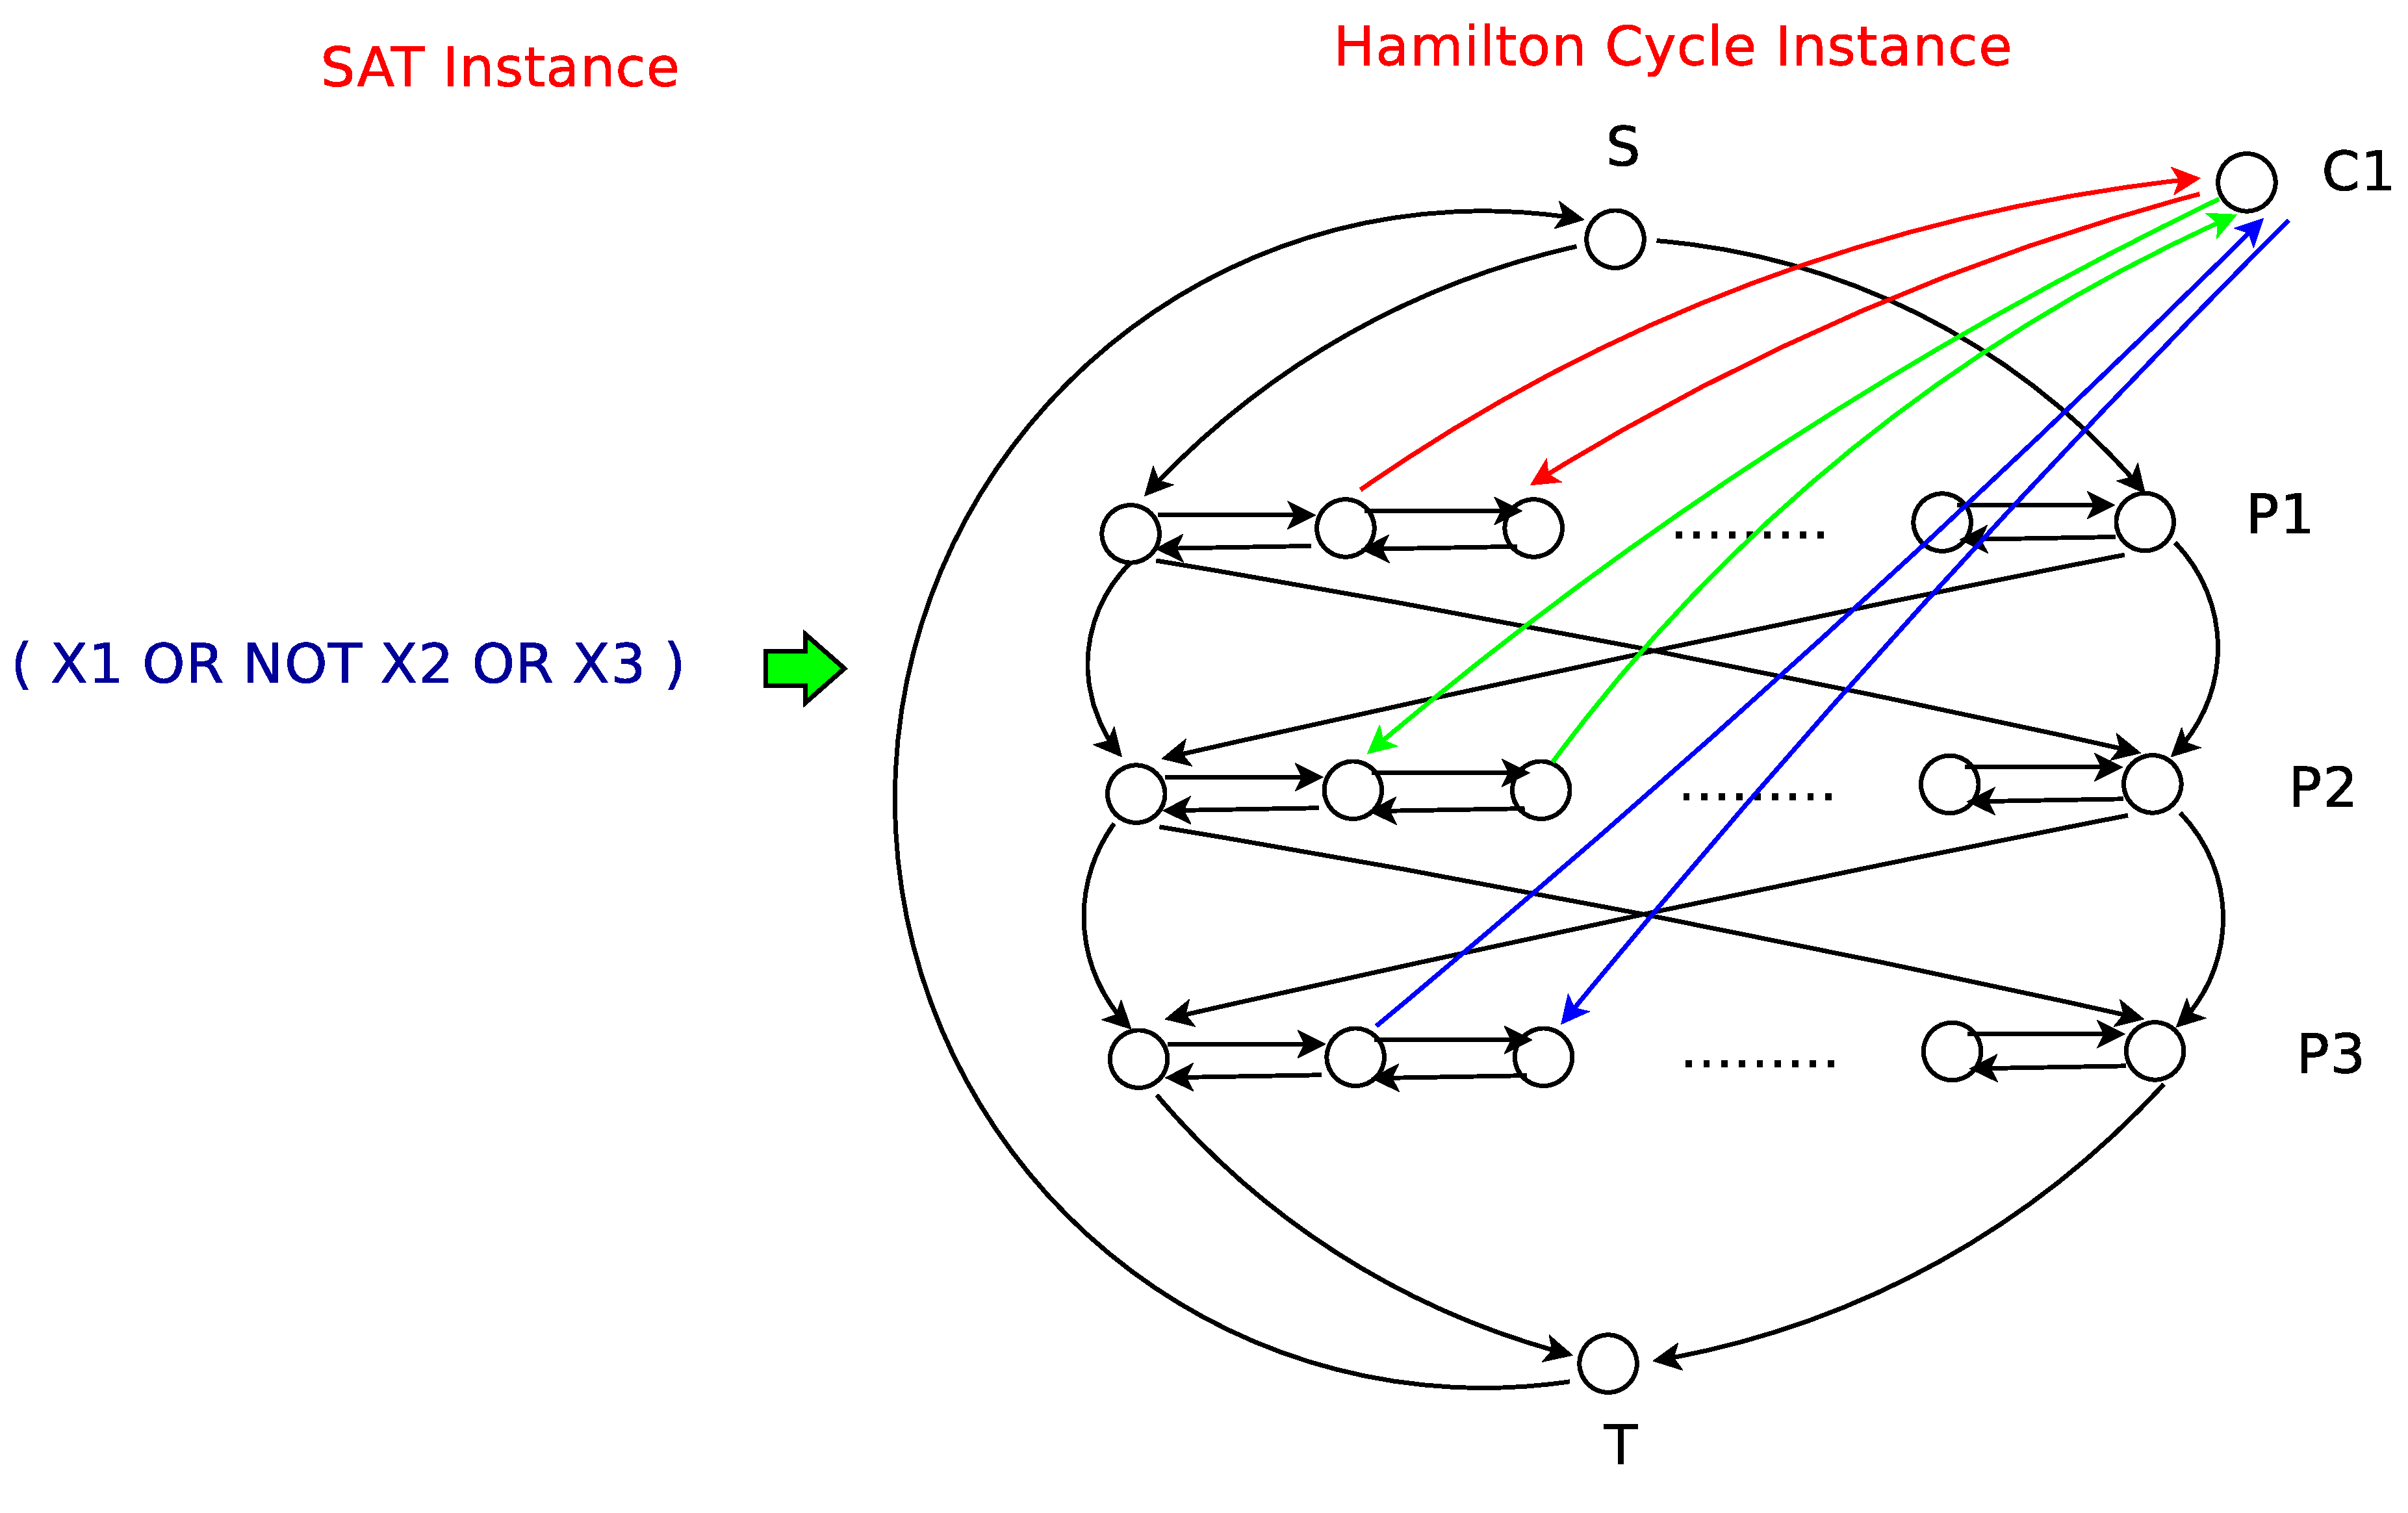
\includegraphics[width=3in]{L3-sathamilton.eps}
\end{figure}
}

\frame{
\frametitle{ How does a gadget work? } 

\begin{itemize}
 \item 
\texttt{TRUE} assignment $\Rightarrow$ a cycle. We travel line $P_i$ from left to right if $x_i=\texttt{TRUE}$, and travel from right to left if $x_i = \texttt{FALSE}$.
 \item 
For example: $x_1 = \texttt{TRUE}$, $x_2 = \texttt{FALSE}$, $x_3=\texttt{TRUE}$ 
\end{itemize}
\begin{figure}
 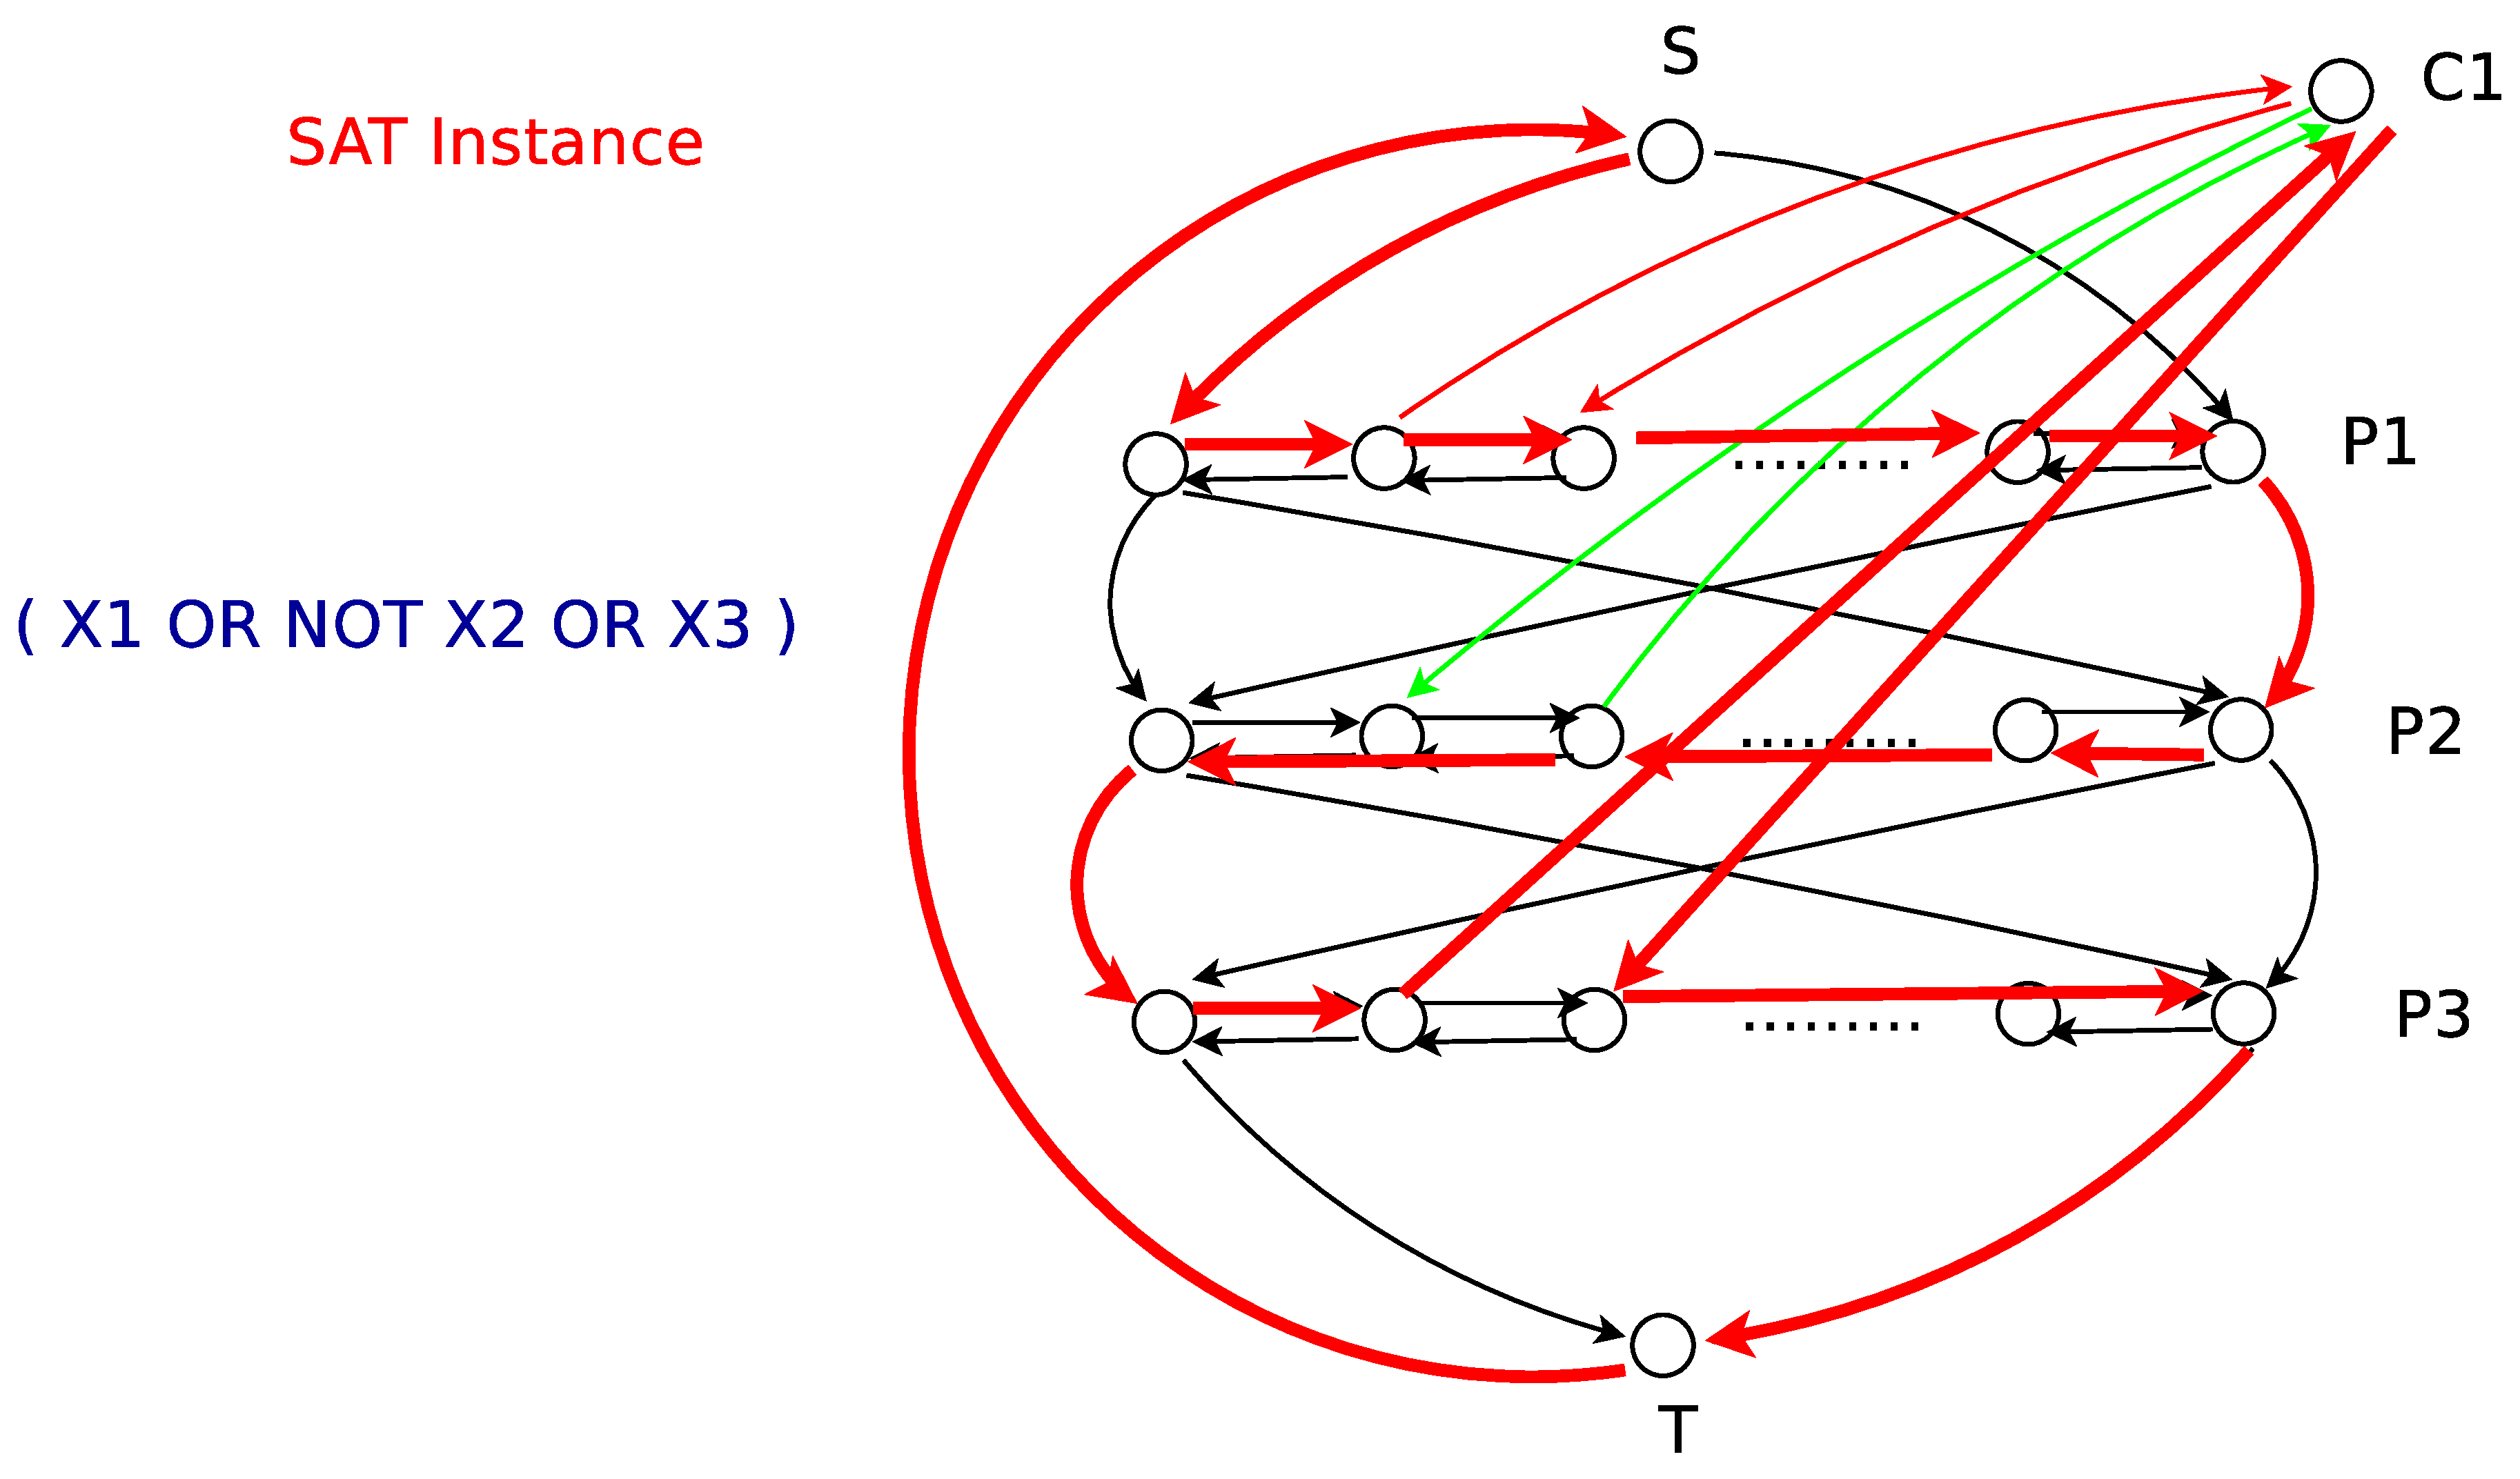
\includegraphics[width=3in]{L3-sathamilton-sat.eps}
\end{figure}
}

\frame{
\frametitle{How does a gadget work? } 
\begin{itemize}
 \item 
\texttt{FALSE} assignment $\Rightarrow$ cannot visit $C$ node. We travel line $P_i$ from left to right if $x_i=\texttt{TRUE}$, and travel from right to left if $x_i = \texttt{FALSE}$.
 \item 
For example: $x_1 = \texttt{FALSE}$, $x_2 = \texttt{TRUE}$, $x_3=\texttt{FALSE}$. We have no chance to visit $C$.
\end{itemize}
\begin{figure}
 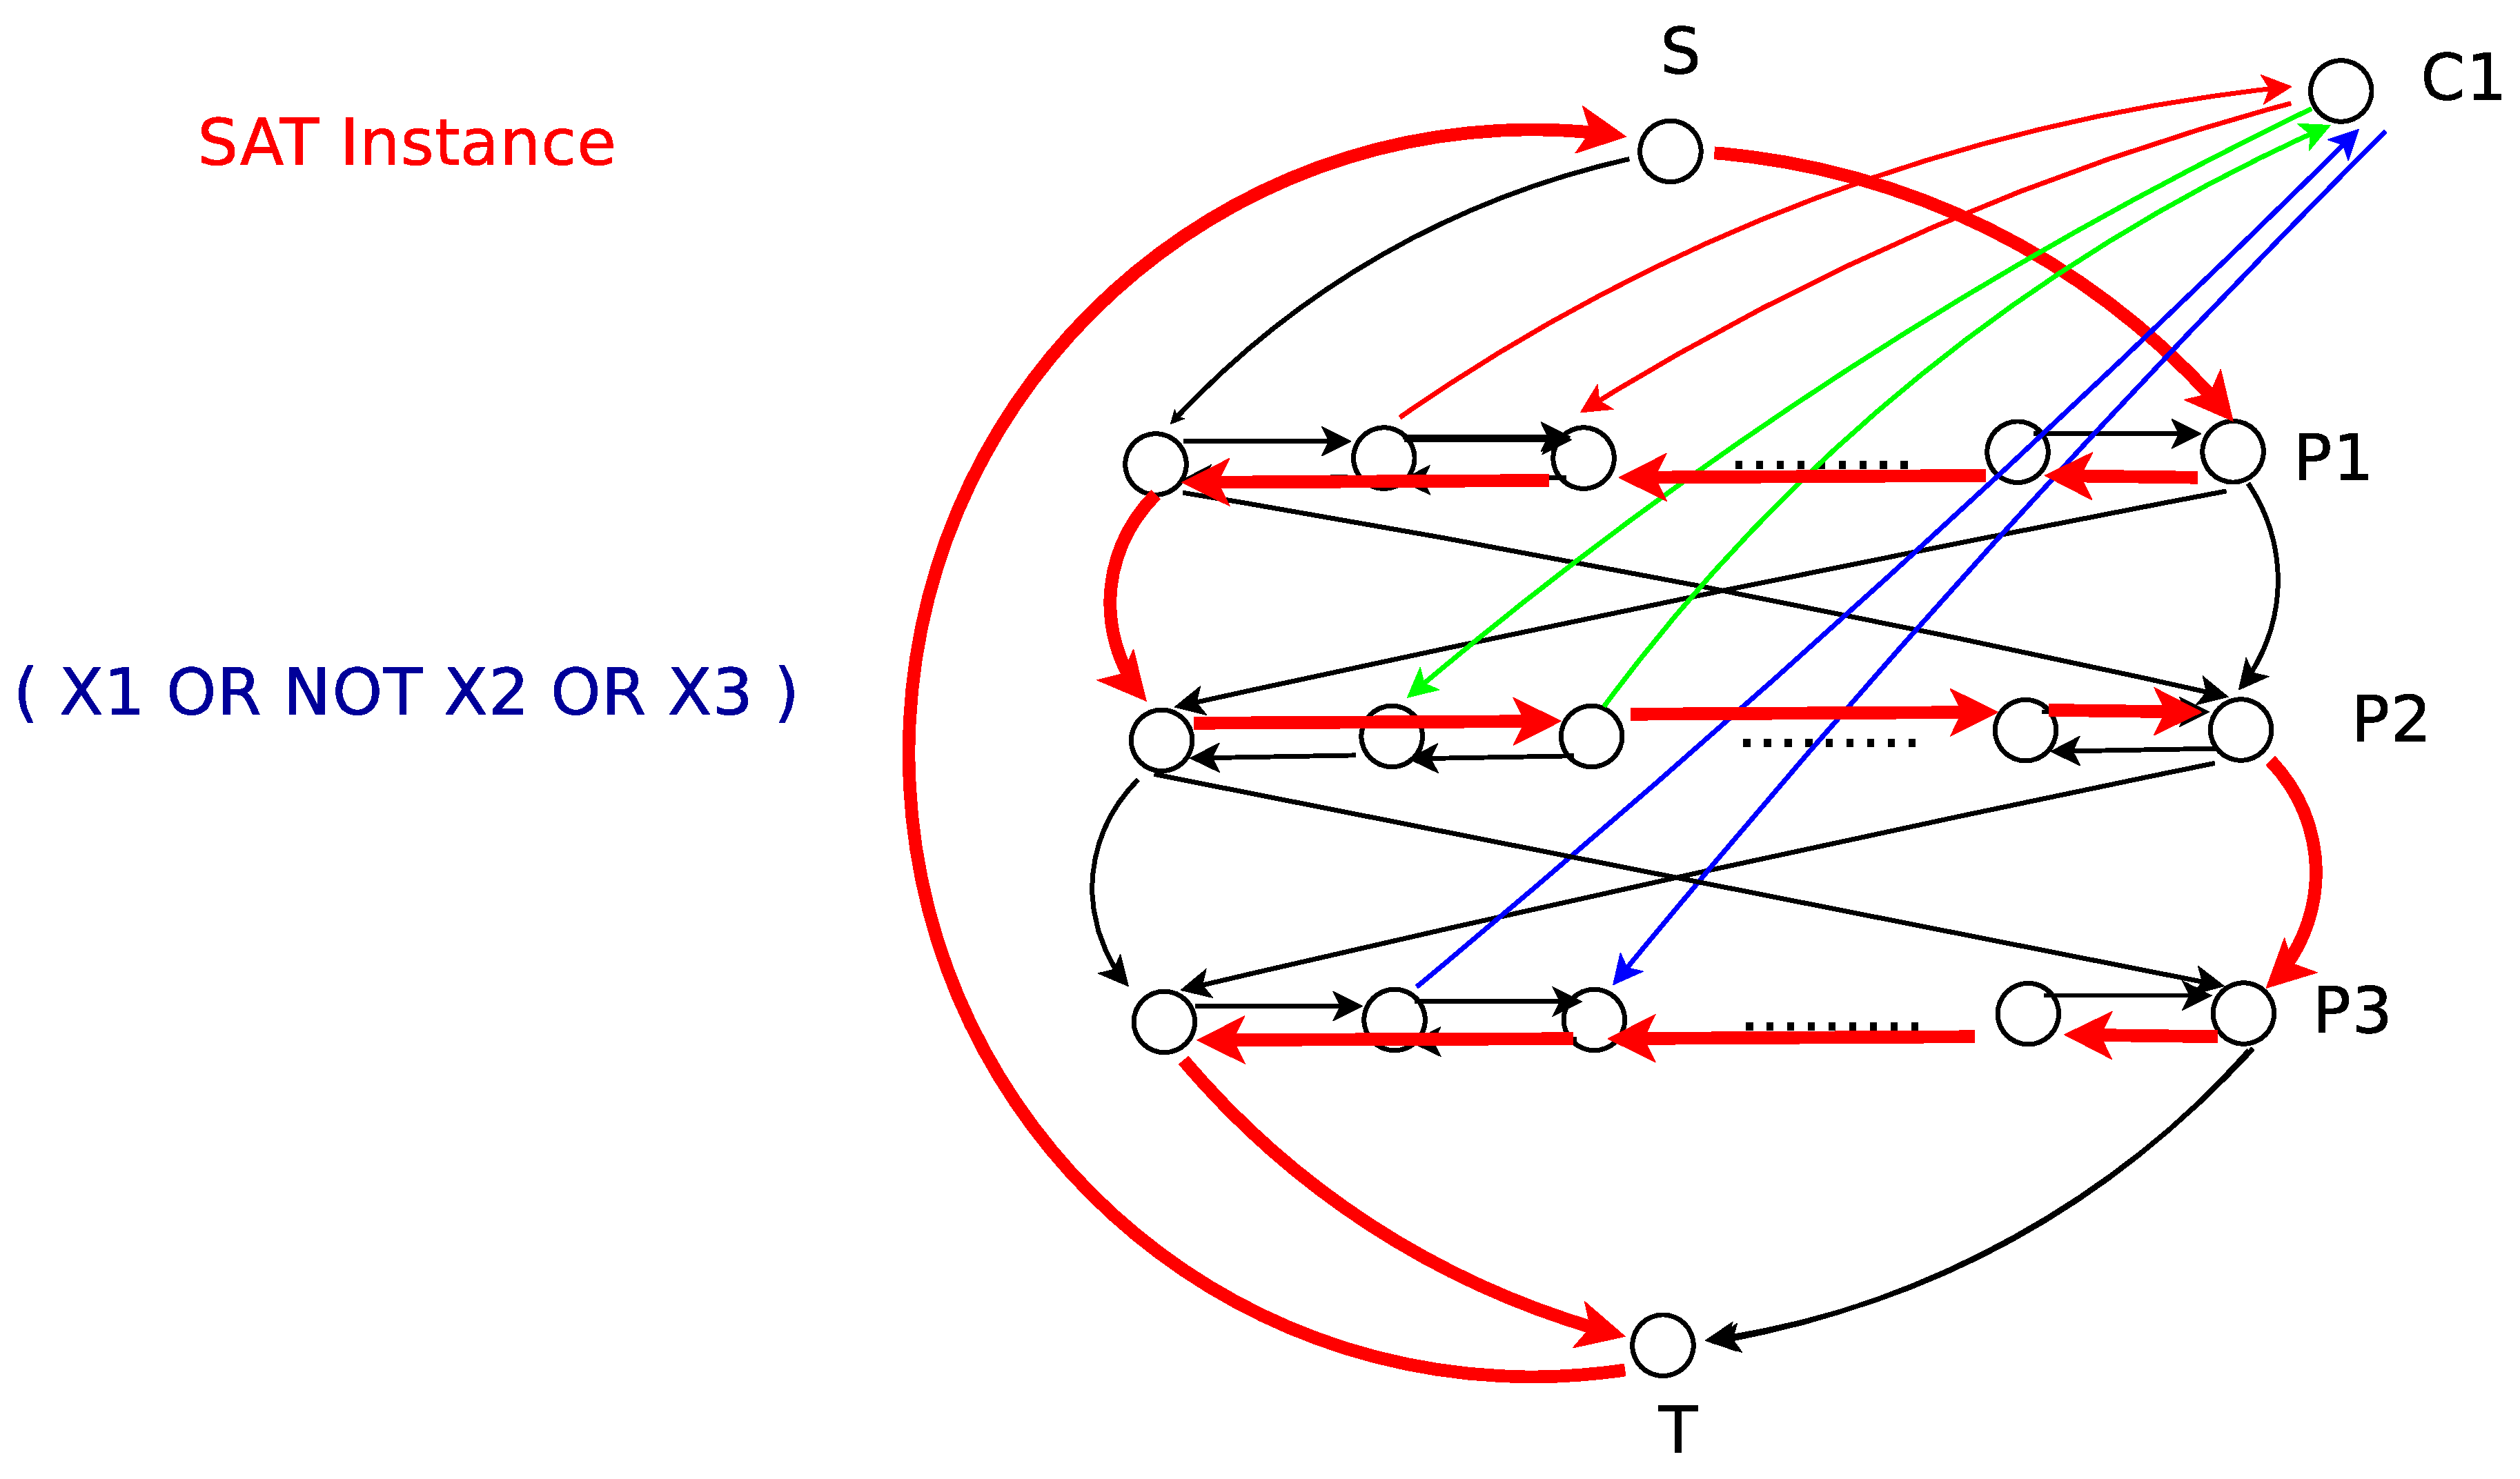
\includegraphics[width=3in]{L3-sathamilton-unsat.eps}
\end{figure}
}


\frame{
\frametitle{Reduction {\sc 3SAT} $\le_P$ {\sc Hamilton Cycle} }

\begin{itemize} 
 \item  \textcolor{blue}{\bf Equivalence:} 
\begin{Proof} 
\begin{itemize}
\begin{footnotesize}
 \item 
Suppose $\phi$ can be satisfied by an assignment; \\
\item 
Starting from $s$; travel line $i$ from left to right if $x_i = \texttt{TRUE}$; otherwise from right to left; \\
\item 
If $C_j$ is satisfied by literal $x_i$ or $\neg x_i$, then travel $C_j$ when traveling line $i$; \\
\item 
Return to $s$ from $t$ finally; \\ 
\item 
This way, all nodes will be visited exactly once. 
\end{footnotesize}
\end{itemize}
\end{Proof}
\end{itemize}
\begin{figure}
 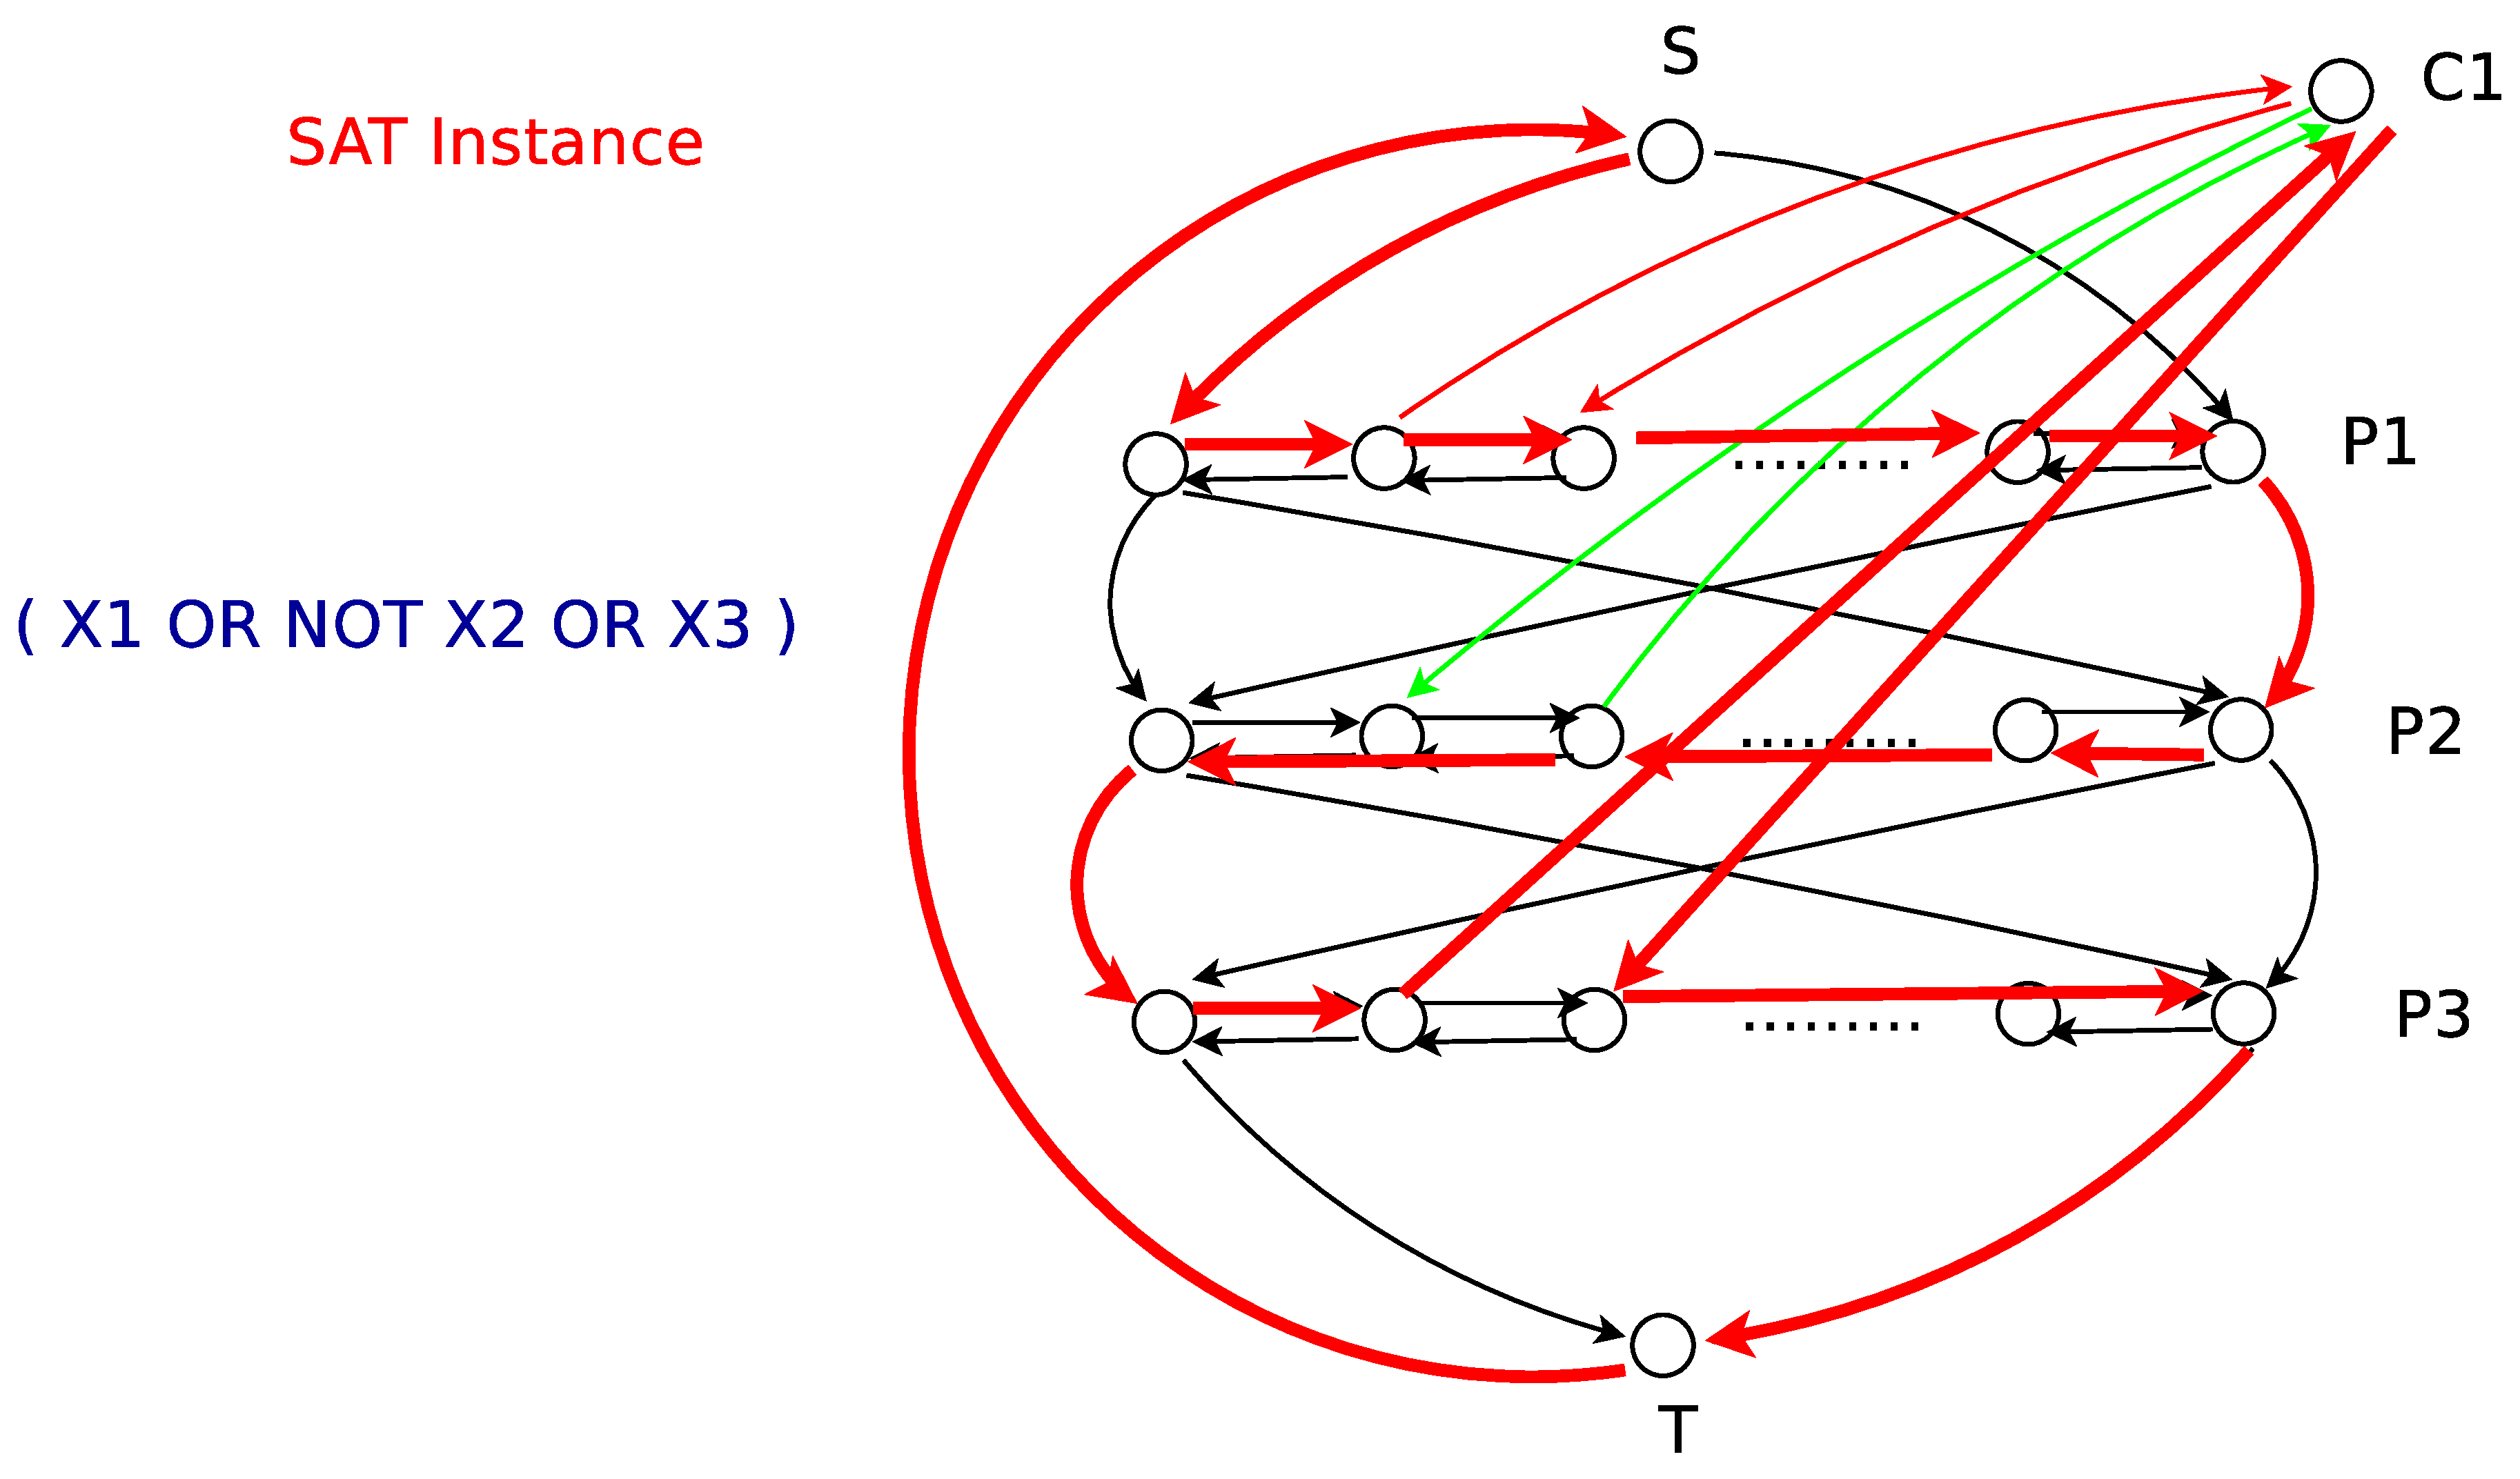
\includegraphics[width=2.5in]{L3-sathamilton-sat.eps}
\end{figure}
} 


\frame{
\frametitle{Reduction {\sc 3SAT} $\le_P$ {\sc Hamilton Cycle}: Equivalence}

\begin{itemize} 
 \item  \textcolor{blue}{\bf Equivalence:} 

\begin{Proof}
\begin{itemize}
 \item 
Suppose there is a Hamilton cycle;   \\
\item 
Assign $x_i = \texttt{TRUE}$ iff  line $i$ are visited from left to right; \\
\item 
This assignment satisfies $\phi$; 
\item 
Each clause $C_j$ is satisfied. Why? 
\end{itemize}
\end{Proof}
\end{itemize}

\begin{figure}
 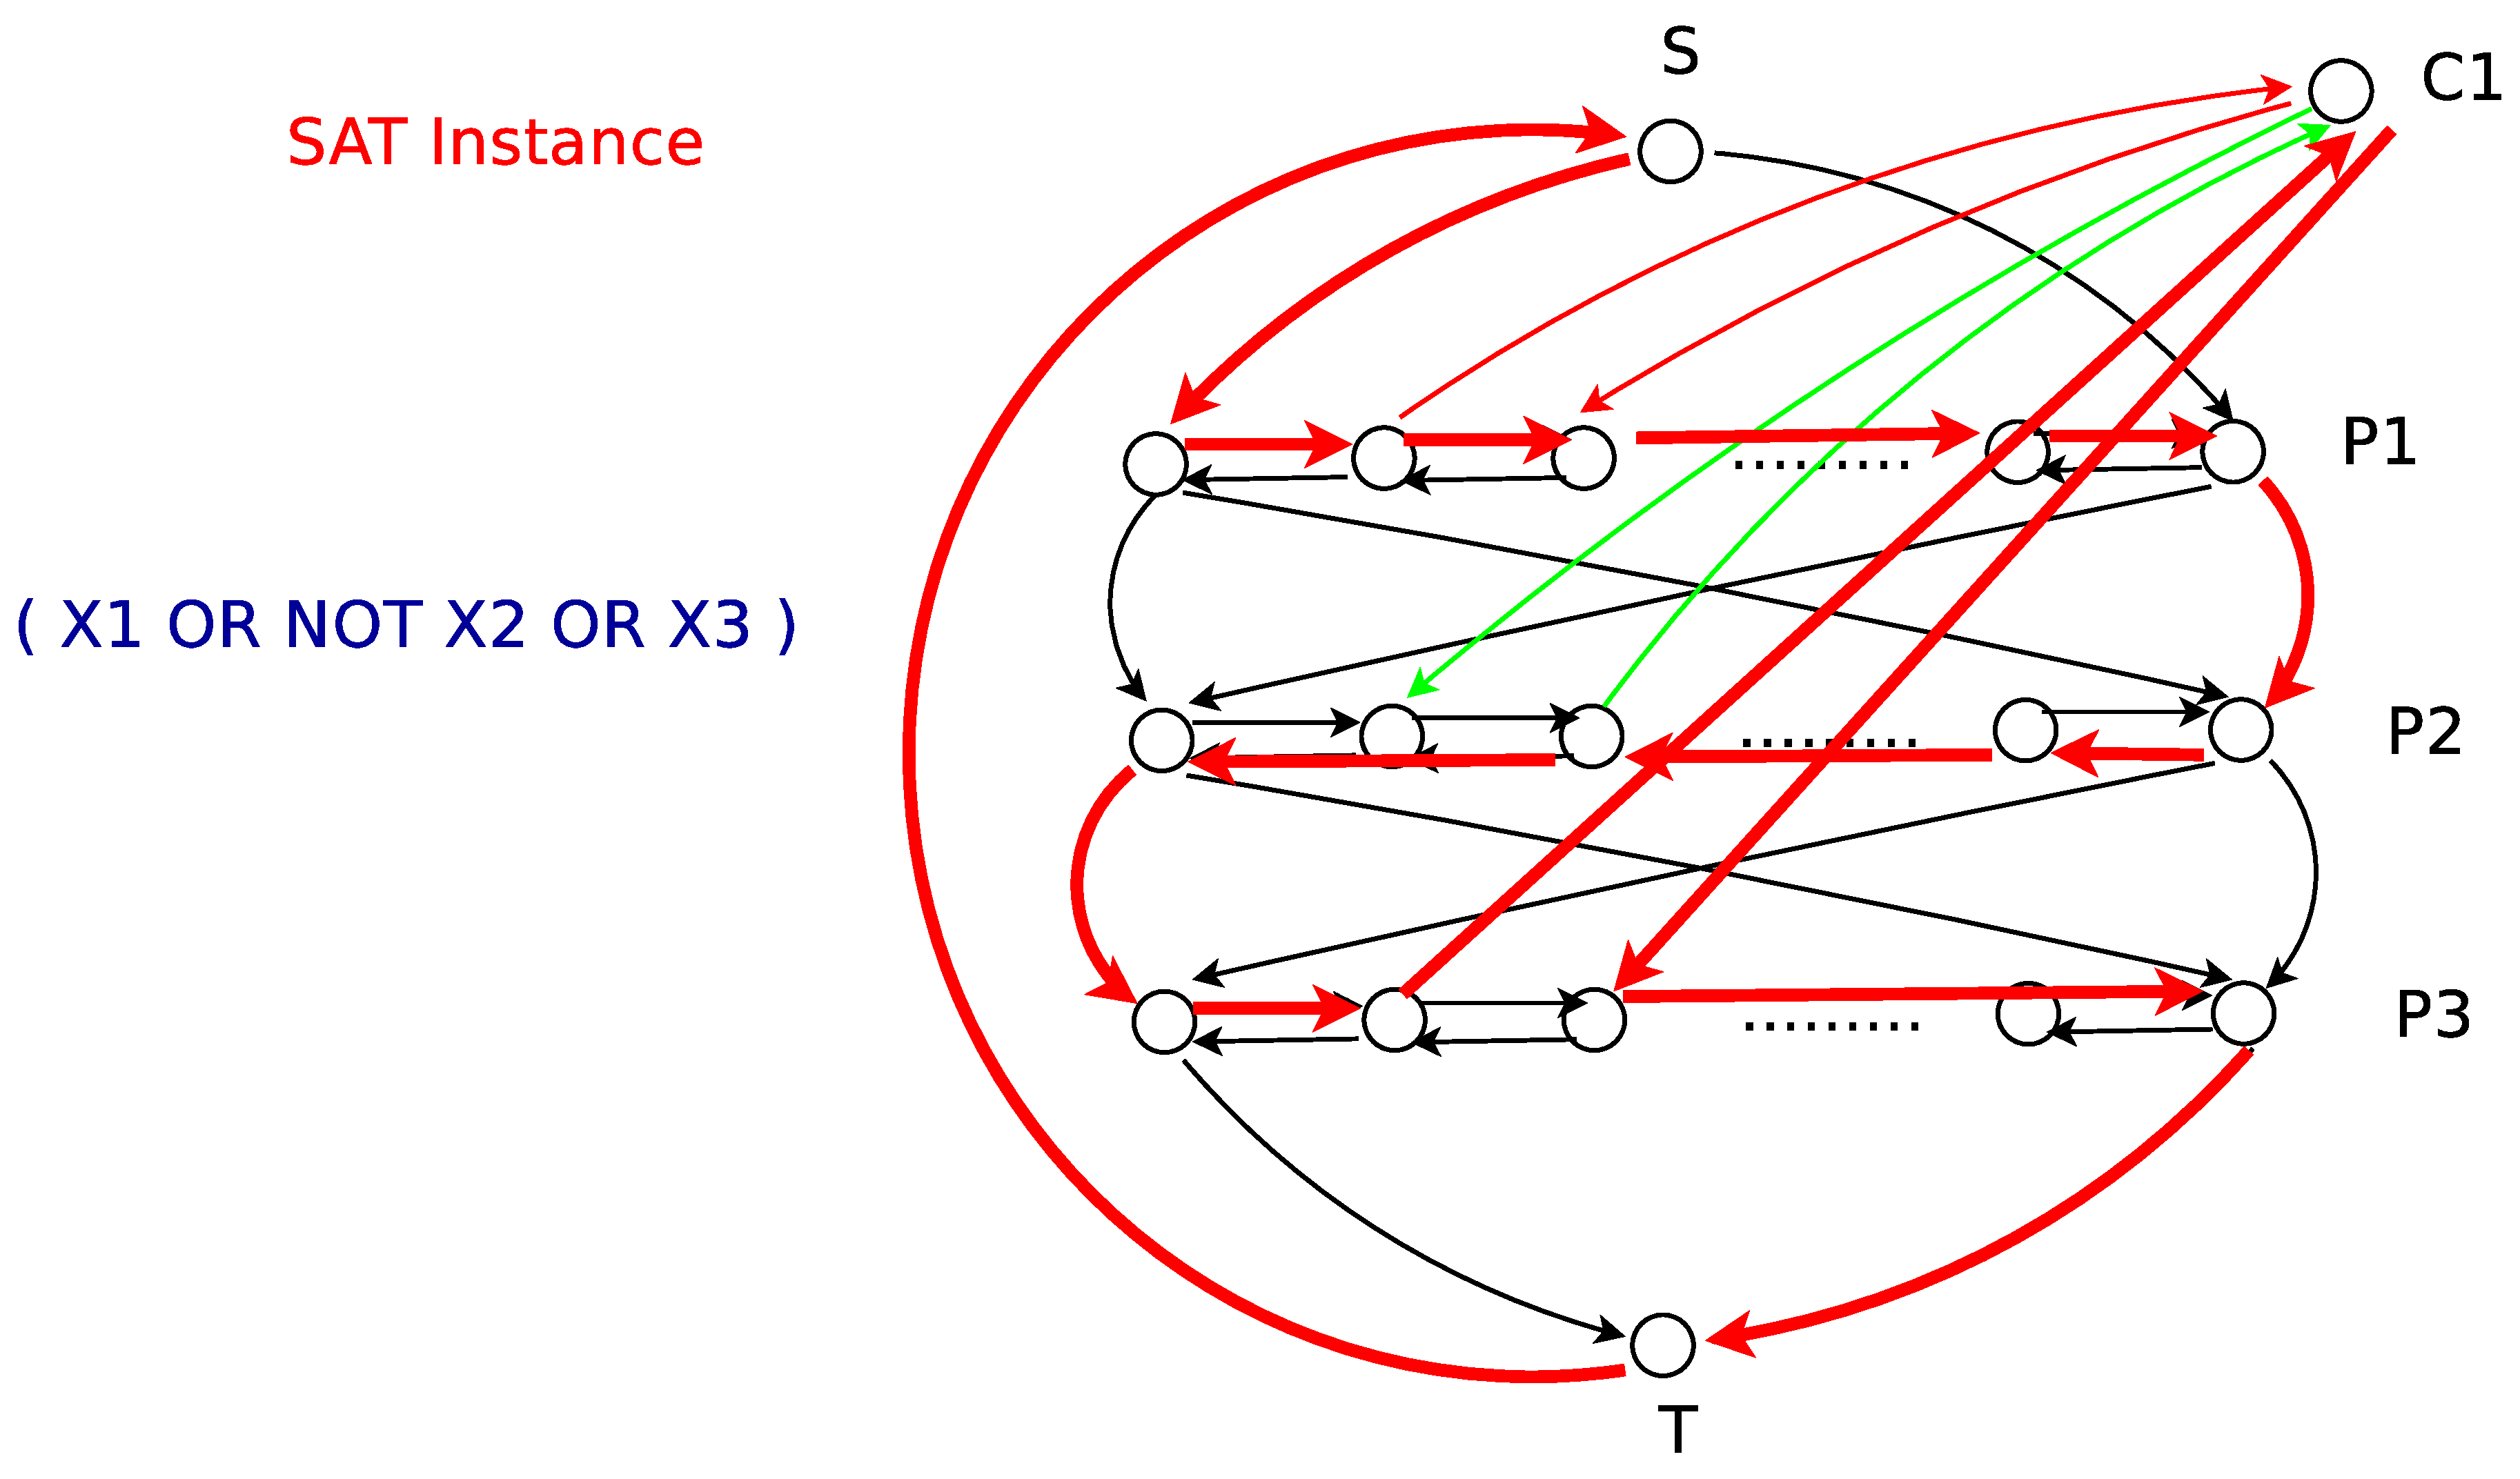
\includegraphics[width=2.5in]{L3-sathamilton-sat.eps}
\end{figure}

}

\frame{
\frametitle{}
\begin{block}{}
 A simple reduction:  {\sc Hamilton Cycle} $\le_P$ {\sc TSP (Traveling Salesman Problem) }.
\end{block}
}

\frame{
\frametitle{ {\sc TSP (Traveling Salesman Problem) } }
Intuition: A salesman tries to travel $n$ cities with the shortest tour. 

\begin{figure}
 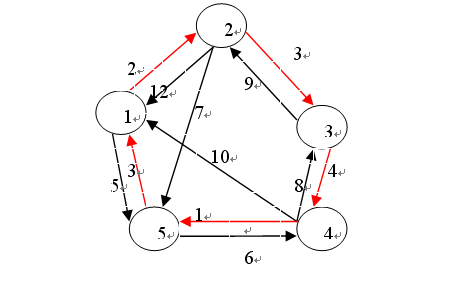
\includegraphics[width=3in] {tsp1.png}
\end{figure}

The tour path with the shortest length is  $1, \ 2, \ 3, \ 4, \ 5, \ 1$ with red color. 
}



\frame{
\frametitle{ {\sc TSP (Traveling Salesman Problem) } }
Optimal tour of 49 cities in the USA (solved by Dantzig, Fulkerson, and Johnson in 1954).


\begin{figure}
 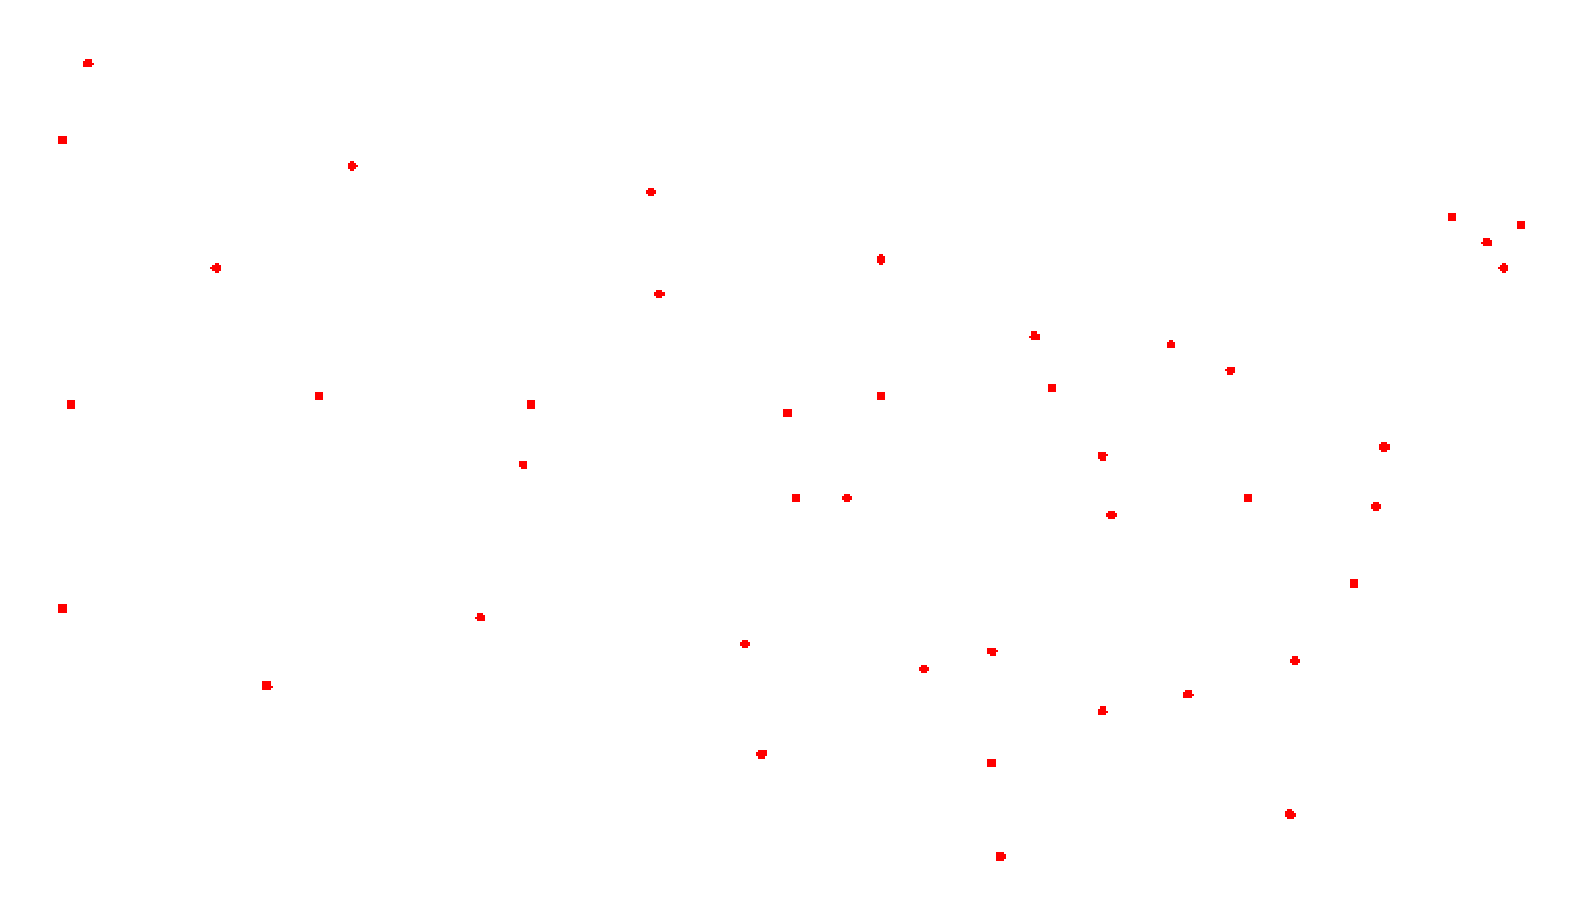
\includegraphics[width=1.8in] {L3-TSP42cities-map.eps}
\end{figure}
\begin{figure}
 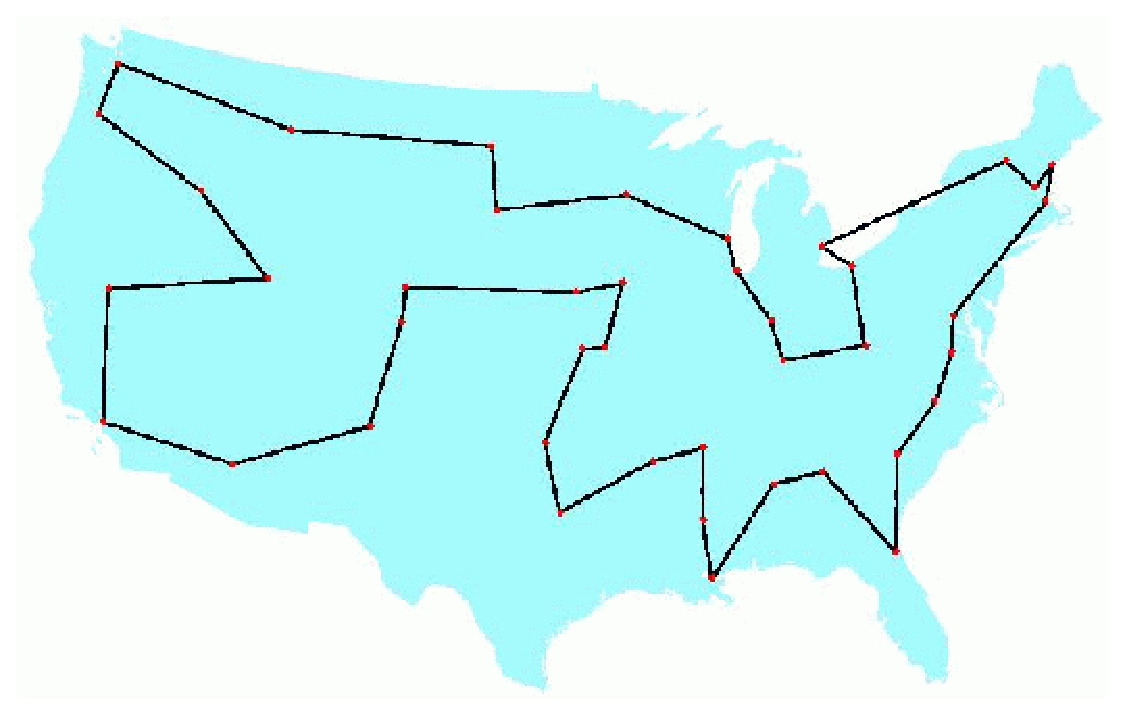
\includegraphics[width=1.8in] {L3-TSP42cities.eps}
\end{figure}

Origin: Karl Menger (1920), Mahalanobis (1940), Jensen (1942), Gosh (1948), Marks (1948) \\

}


\frame{
\frametitle{ {\sc TSP (Traveling Salesman Problem) research progress} }


\begin{figure}
 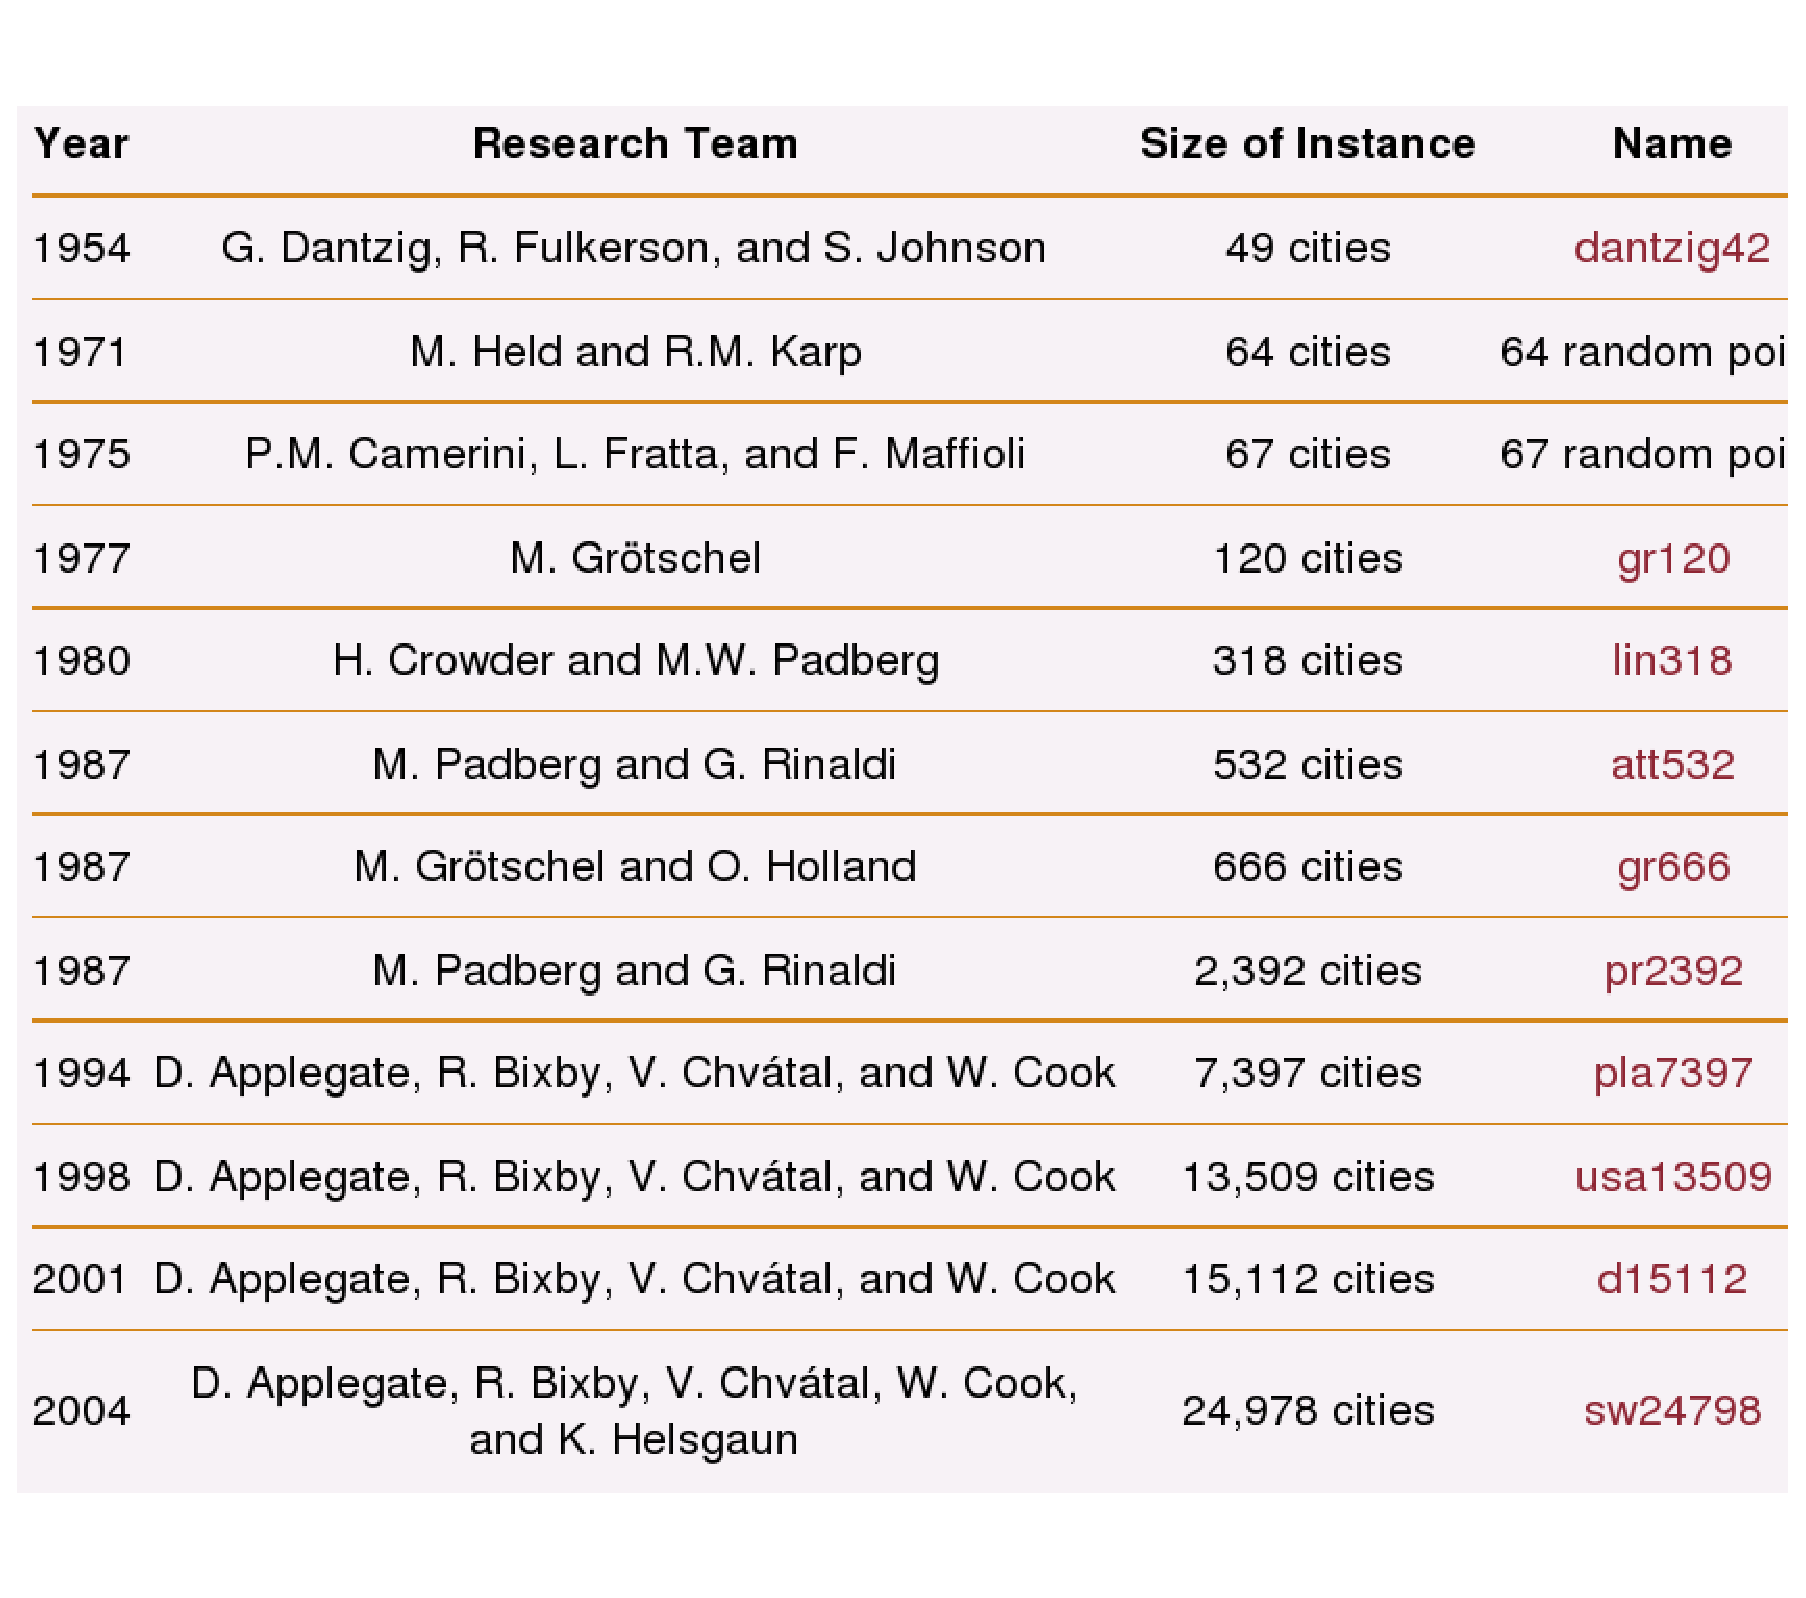
\includegraphics[width=2.8in] {L3-TSPprogress.eps}
\end{figure}

(Excerpted from http://www.tsp.gatech.edu/history/milestone.html.)
}

\frame{
\frametitle{TSP cont'd}

 \begin{itemize}
 \item Practical problem: \\
 	path planning: the most efficient motion of a robotic arm that drill $n$ holes on a VLSI chip;
\end{itemize}
\begin{block}{Formalized Definition:}
 {\bf Input:} Given a graph $G=<V,E>$, distance $d: E \rightarrow R$, and a bound $B$; \\
 {\bf Output:} is there a Hamilton cycle with total distance less than $B$? 
\end{block}

}




% \frame{
% \frametitle{Key observation: A special case of TSP}
% 
% 
% $G'$ has a tour with total distance not great than $0$ iff there is a Hamilton cycle in $G$. 
% 
% 
% \begin{figure}
%  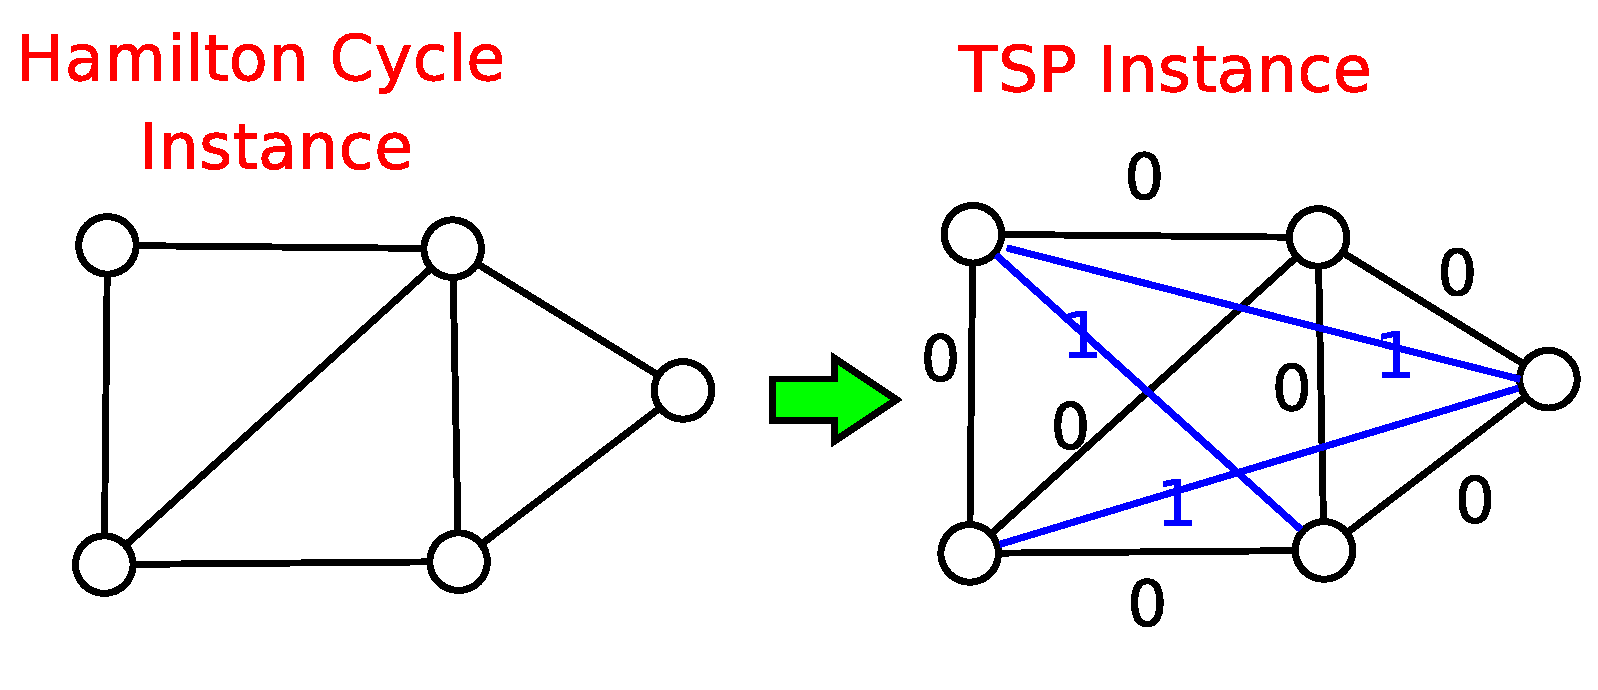
\includegraphics[width=3in] {L3-hamiltoncycletsp.eps}
% \end{figure}
% 
% }

\frame{
\frametitle{Reduction: {\sc Hamilton Cycle} $\le_P$ {\sc TSP} }
\begin{itemize}
 \item 
{\bf Transformation}: for a {\sc Hamilton Cycle} instance $G=<V, E>$, we construct a {\sc TSP} instance as follows: $G'$: a complete graph with $n$ node, $d(u, v) = 0$ if $(u, v) \in E$; otherwise $d(u,v)=+\inf$. Let $B = 0$; 

\begin{figure}
 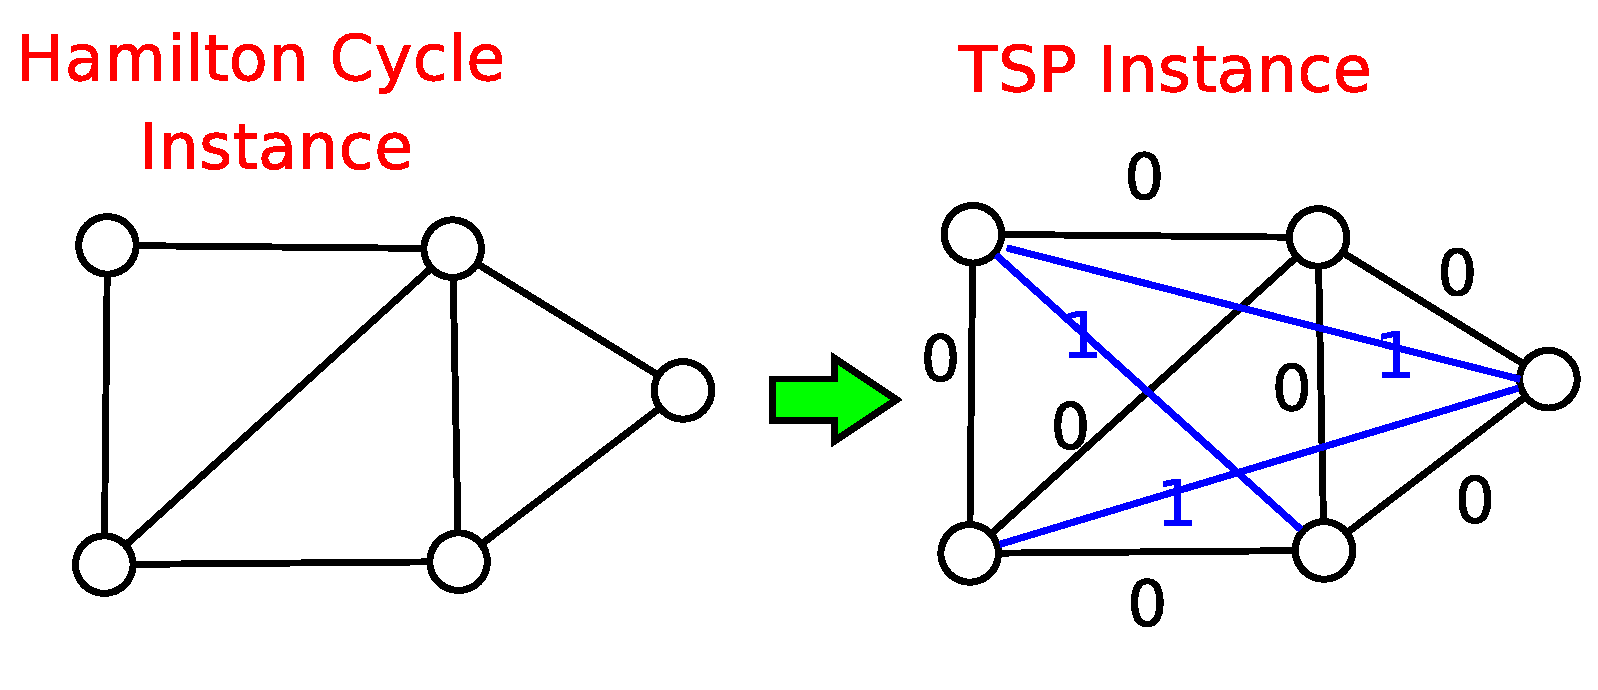
\includegraphics[width=3in] {L3-hamiltoncycletsp.eps}
\end{figure}


\item 
{\bf Equivalence}:  a tour with total distance $\le 0$ in $G'$ corresponds to a Hamilton cycle in $G$. 

\end{itemize}
}


\frame{
\frametitle{}
\begin{block}{}
 Extended reading: Computing Hamiltonian path using DNA computer 
\end{block}
}

\frame{
\frametitle{Molecular Computation of Solutions to Combinatorial Problems, Leonard M. Adleman [1994]} 
\begin{figure}
 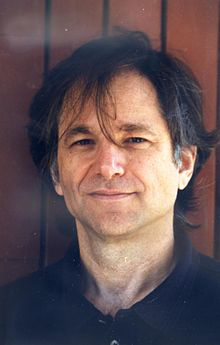
\includegraphics[width=0.8in] {Adleman.png}
\end{figure}
\begin{itemize}
\item 
The tools of molecular biology were used to solve an instance of the directed Hamiltonian path problem. 
\item  A small graph was encoded in molecules of DNA, and the "operations" of the computation were performed with standard protocols and enzymes. 
\item This experiment demonstrates the feasibility of carrying out computations at the molecular level.
\end{itemize}

}

\frame{
\frametitle{Representing a Hamiltonian instance using DNA} 
\begin{figure}
 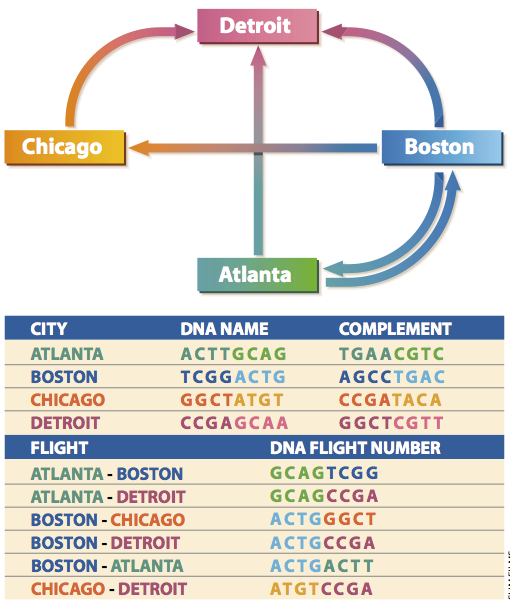
\includegraphics[width=2.8in] {DNAComputer1.png}
\end{figure}
} 


\frame{
\frametitle{A path generated during DNA synthesis process} 
\begin{figure}
 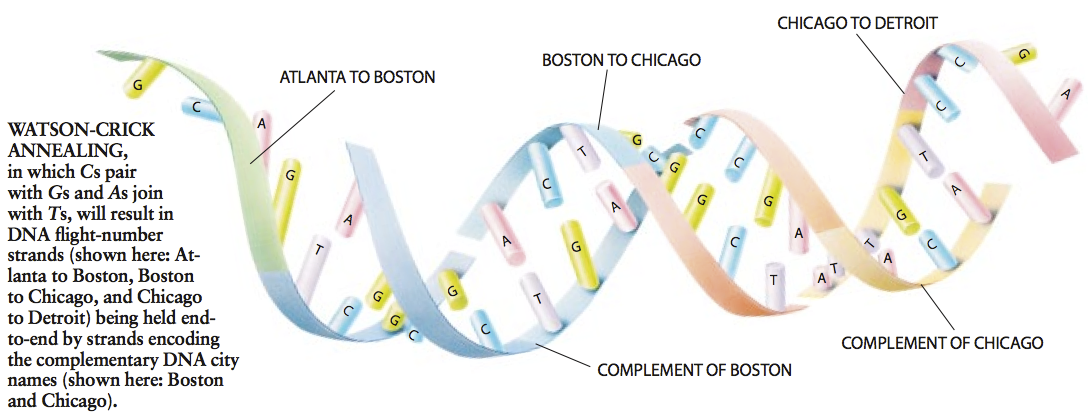
\includegraphics[width=4.5in] {DNAComputer2.png}
\end{figure}
} 



\frame{
\frametitle{}
\begin{block}{}
 A simple reduction:  {\sc SAT} $\le_P$ {\sc Graph Coloring}
\end{block}
}


\frame{
\frametitle{ {\sc Graph Coloring} problem }
\begin{itemize}
 \item 
Practical problem:  \\ {\it 
Consider assigning one of the $k$ wavelengths to $n$ wireless devices. If two devices are sufficiently close to each other, we should assign them with different wavelengths to prevent interference.  }

\begin{block}{Formalized Definition:}
 {\bf Input:} A graph $G=<V,E>$, an integer $k$; \\
 {\bf Output:} Is there a  $k-coloring$ of $G$ such that each node has a color, but the two endpoints of an edge have different colors? 
\end{block}
\end{itemize}
}

\frame{
\frametitle{An example}
\begin{figure}
 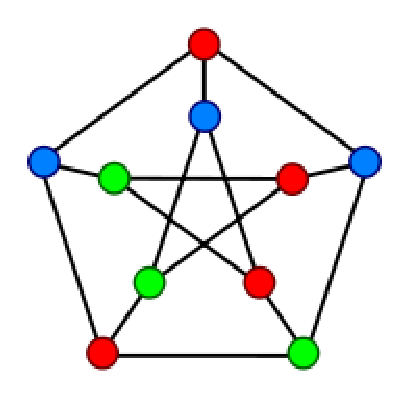
\includegraphics[width=1.5in] {180px-Petersen_graph_3-coloring.eps}
\end{figure}
A proper vertex coloring of the Petersen graph with $3$ colors, the minimum number possible.
} 

\frame{
\frametitle{Graph coloring: a brief introduction }
There are three types of coloring: 
\begin{enumerate}
 \item Vertex coloring: coloring the vertices of a graph such that no two adjacent vertices share the same color; 
 \item Edge coloring: coloring edges so that no two adjacent edges share the same color
 \item Face coloring: (planar graph) coloring faces or region so that no two faces that share a boundary have the same color.
 \end{enumerate}

\begin{tiny}
 


\begin{figure}
 \begin{minipage}{0.3\textwidth}
 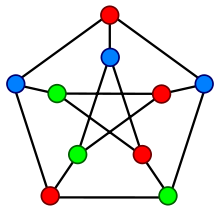
\includegraphics[width=\textwidth]{L3-vertexcoloring.png}
 \caption{ \begin{tiny} Peterson graph \end{tiny} }
\end{minipage}
\begin{minipage}{0.3\textwidth}
 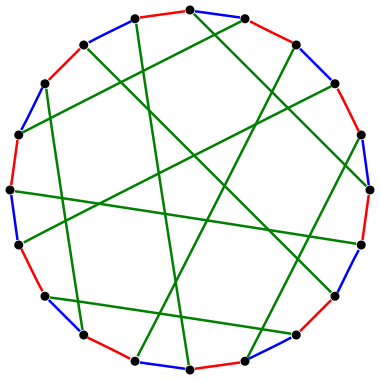
\includegraphics[width=\textwidth]{L3-edgecoloring.png}
 \caption{\begin{tiny} Desargues graph: the complement of Peterson graph \end{tiny}}
\end{minipage}
\begin{minipage}{0.3\textwidth}
 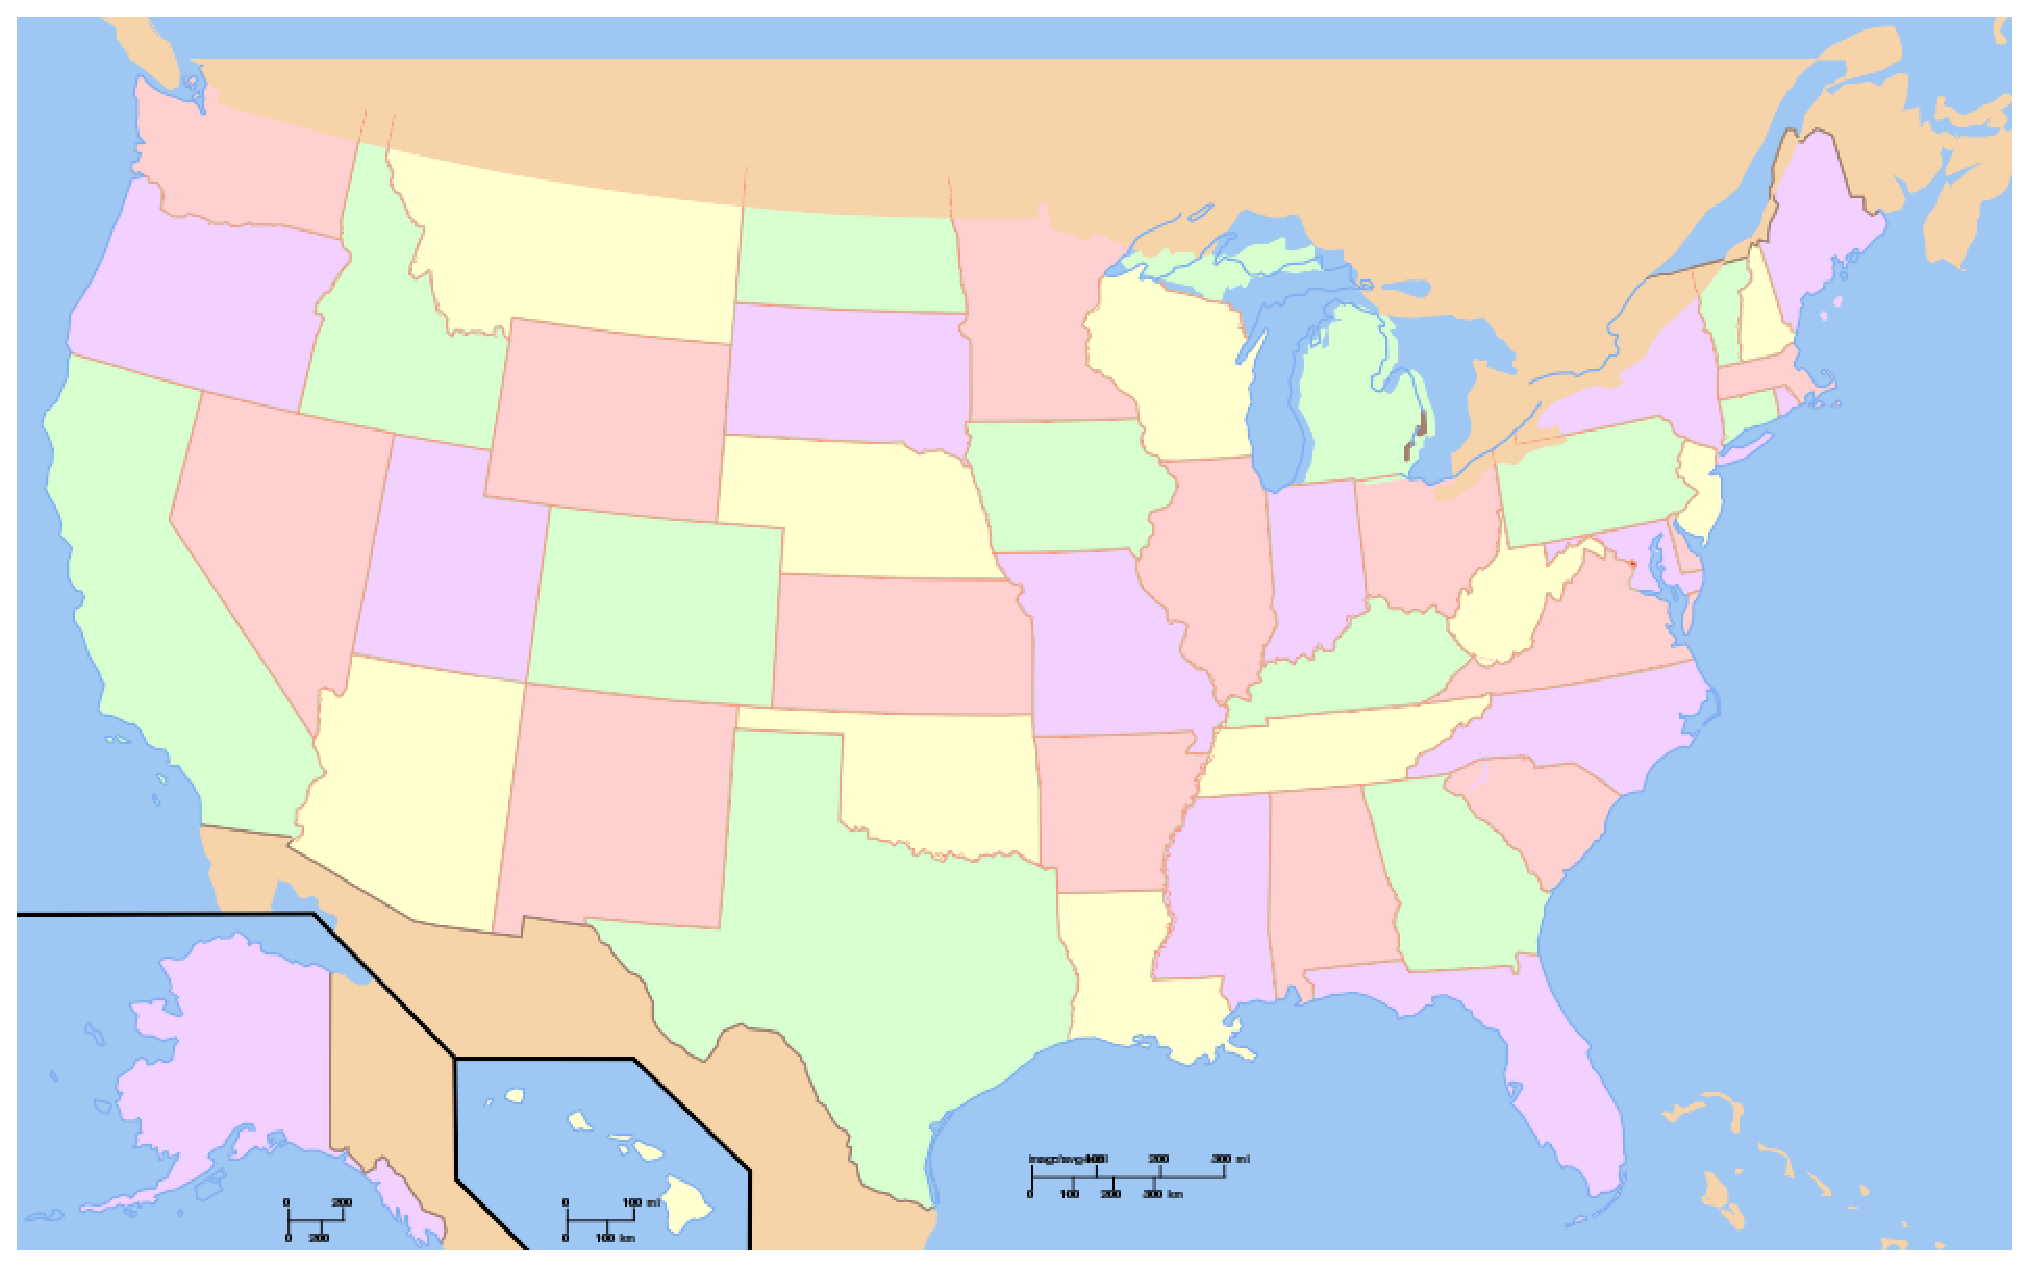
\includegraphics[width=\textwidth]{L3-facecoloring.eps}
 \caption{\begin{tiny}  USA map \end{tiny}}
\end{minipage}
\end{figure}
\end{tiny}

}

\frame{
\frametitle{Transforming {\sc Edge Coloring} into {\sc Vertex Coloring}}

Edge coloring $\Rightarrow$ vertex coloring (line graph ): an edge coloring of a graph is just a vertex coloring of its line graph.  
\begin{figure}
 \begin{minipage}{0.4\textwidth}
 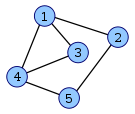
\includegraphics[width=\textwidth]{L3-linegraph1.png} 
 \end{minipage}
 \begin{minipage}{0.4\textwidth}
 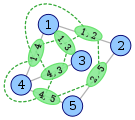
\includegraphics[width=\textwidth]{L3-linegraph2.png} 
 \end{minipage}
\end{figure}
 \footnote{The 3 slides were excerpted from Wiki::Graph Coloring} 
} 


\frame{
\frametitle{Transforming {\sc Face Coloring} into {\sc Vertex Coloring} }
 
 
 Face coloring $\Rightarrow$ vertex coloring (graph dual ): a face coloring of a planar graph is just a vertex coloring of its planar dual.


\begin{figure}
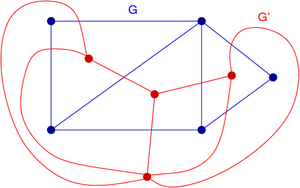
\includegraphics[width=2in]{L3-dualgraph.png} 
\end{figure}

}

\frame{
\frametitle{Planar graph: 4 coloring}

 \begin{itemize}
   \item 
 

 The four-color theorem was proven in 1976 by Kenneth Appel and Wolfgang Haken. 
\item 
It was the first major theorem to be proved using a computer. 
\item 
Appel and Haken's approach started by showing that there is a particular set of 1,936 maps, each of which cannot be part of a smallest-sized counterexample to the four color theorem. 
\item 

Appel and Haken used a special-purpose computer program to confirm that each of these maps had this property.
\end{itemize}

}

\frame{
\frametitle{General graph: $2$-coloring.  }


\begin{itemize}
 \item $2$-coloring is in $P$.  
 \item A graph $G$ can be $2$-coloring iff $G$ is a bi-partitie. 
\end{itemize}

\begin{figure}
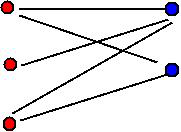
\includegraphics[width=1in]{L3-2coloring.png} 
\end{figure}

}


\frame{
\frametitle{General graph: $k$-coloring ($k\ge 3$) }


\begin{itemize}
 \item Using dynamic programming and a bound on the number of maximal independent sets, k-colorability can be decided in time and space $O(2.445^n)$.

 \item 
 Using the principle of inclusion–exclusion and Yates’s algorithm for the fast zeta transform, k-colorability can be decided in time $O(2^n n)$ for any $k$. 
\item Faster algorithms are known for 3- and 4-colorability, which can be decided in time $O(1.3289^n)$  and $O(1.7504^n)$, respectively.
\end{itemize}
}


\frame{
\frametitle{ Designing gadget: triangle }
\begin{itemize}
\item 
\textcolor{blue}{\bf Triangle:}  Suppose a node has already been colored in Green, one of the other nodes should be Red OR Blue; 
\item 
Hint: can be used to express a Boolean variable since $x_i = \texttt{TRUE} $ \textcolor{red}{\bf OR} $ \texttt{FALSE}$. For example:  Red: True, Blue: False. 
\end{itemize}

\begin{figure}
 \includegraphics[width=3in] {L3-coloringgadgettriangle.eps}
\end{figure}
}


\frame{
\frametitle{ Designing gadget: fork }

\begin{itemize}
\item 
\textcolor{blue}{\bf Fork:} If the three endpoints use all RGB colors, the root cannot be colored. 
\end{itemize} 

\begin{figure}
 \includegraphics[width=3in] {L3-coloringgadgetfork.eps}
\end{figure}
}


\frame{
\frametitle{  Designing gadget: crown }

\begin{itemize}
\item 
\textcolor{blue}{\bf Crown:} $C$ can be colored iff one of the three input is colored in Red.  \\
\item 
Hint: can be used to express a clause since at least one of the three literals should be TRUE. 
\end{itemize} 

\begin{figure}
 \includegraphics[width=2in] {L3-coloringgadgetcrown.eps}
\end{figure}
}

\frame{
\frametitle{ Case 1: the three input of crown = BBB }

\begin{figure}
 \includegraphics[width=2in] {L3-coloringclausecrownBBB.eps}
\end{figure}

$I_1 = B$, $I_2 = B$, $I_3 = B$ $\Rightarrow$ $C$ cannot be colored. 
}

\frame{
\frametitle{ Case 2: the three input of crown = BBR }


\begin{figure}
 \includegraphics[width=2in] {L3-coloringclausecrownBBR.eps}
\end{figure}

$I_1 = B$, $I_2 = B$, $I_3 = R$ $\Rightarrow$ $C$ can be colored. 
}


\frame{
\frametitle{ Case 3: the three input of crown = BRB }


\begin{figure}
 \includegraphics[width=2in] {L3-coloringclausecrownBRB.eps}
\end{figure}

$I_1 = B$, $I_2 = R$, $I_3 = B$ $\Rightarrow$ $C$ can be colored. 
}


\frame{
\frametitle{ Case 4: the three input of crown = BRR }


\begin{figure}
 \includegraphics[width=2in] {L3-coloringclausecrownBRR.eps}
\end{figure}

$I_1 = B$, $I_2 = R$, $I_3 = R$ $\Rightarrow$ $C$ can be colored. 
}


\frame{
\frametitle{ Case 5: the three input of crown = RBB }


\begin{figure}
 \includegraphics[width=2in] {L3-coloringclausecrownRBB.eps}
\end{figure}

$I_1 = R$, $I_2 = B$, $I_3 = B$ $\Rightarrow$ $C$ can be colored. 
}



\frame{
\frametitle{ Case 6: the three input of crown = RBR }


\begin{figure}
 \includegraphics[width=2in] {L3-coloringclausecrownRBR.eps}
\end{figure}

$I_1 = R$, $I_2 = B$, $I_3 = R$ $\Rightarrow$ $C$ can be colored. 
}


\frame{
\frametitle{ Case 7: the three input of crown = RRB }


\begin{figure}
 \includegraphics[width=2in] {L3-coloringclausecrownRRB.eps}
\end{figure}

$I_1 = R$, $I_2 = R$, $I_3 = B$ $\Rightarrow$ $C$ can be colored. 
}


\frame{
\frametitle{ Case 8: the three input of crown = RRR }


\begin{figure}
 \includegraphics[width=2in] {L3-coloringclausecrownRRR.eps}
\end{figure}

$I_1 = R$, $I_2 = R$, $I_3 = R$ $\Rightarrow$ $C$ can be colored. 
}

\frame{
\frametitle{{\sc SAT} $\le_P$ {\sc 3-Coloring}: Transformation }
\begin{itemize}
\item Transformation: a variable $\Rightarrow$ a triangle; 
\end{itemize}

\begin{figure}
 \includegraphics[width=2in] {L3-coloringvariables.eps}
\end{figure}

}

\frame{
\frametitle{{\sc SAT} $\le_P$ {\sc 3-Coloring}: Transformation  cont'd}
\begin{itemize}
 \item 
 Transformation: Clause $\Rightarrow$ connecting inputs with literals.  
 \item 
 Example: $C = (x_1 \vee \neg x_2 \vee x_3)$ 
\end{itemize}
\begin{figure}
 \includegraphics[width=1.5in] {L3-coloringclause.eps}
\end{figure}

Note: The node $C$ can be colored iff one of the three input is colored in Red, i.e., at least one literal is satisfied.
}


% \frame{
% \frametitle{ True assignment $\Rightarrow$ 3-Coloring }
% 
% $x_1 = T$,  $x_2 = T$, $x_3 = F$.
% \begin{figure}
%  \includegraphics[width=2in] {L3-coloringclause-satcase1.eps}
% \end{figure}
% }

 \frame{
 \frametitle{ True assignment $\Rightarrow$ 3-Coloring }
\begin{itemize}
 \item 
 Clause $\Rightarrow$ connecting inputs with literals.  
 \item 
 Example: $C = (x_1 \vee \neg x_2 \vee x_3)$ 
 \item 
 True assignment: $x_1 = T$,  $x_2 = T$, $x_3 = F$.
\end{itemize}

 \begin{figure}
  \includegraphics[width=1.8in] {L3-coloringclause-satcase1.eps}
 \end{figure}
 }

\frame{
\frametitle{ False assignment $\Rightarrow$ No 3-Coloring }
\begin{itemize}
 \item 
Clause $\Rightarrow$ connecting inputs with literals.  
 \item 
 Example: $C = (x_1 \vee \neg x_2 \vee x_3)$ 
 \item 
False assignment: $x_1 = F$,  $x_2 = T$, $x_3 = F$.
\end{itemize}

\begin{figure}
 \includegraphics[width=1.8in] {L3-coloringclause-unsat.eps}
\end{figure}
}

\frame{
\frametitle{Reduction: {\sc SAT} $\le_P$ {\sc 3-Coloring} }
\begin{Proof}
$\Rightarrow $ \\
\begin{itemize}
 \item 
Consider a true assignment;  \\
\item 
Color $v_i$ Red if $x_i = TRUE$; otherwise $Blue$; \\
\item 
This is a 3-Coloring. ( $C$ can be colored unless ALL 3 input are in Blue. )
\end{itemize}

$\Leftarrow $ \\
\begin{itemize}
 \item 
Consider a 3-Coloring; (w.l.o.g, suppose node $T$ is in Red, $F$ is in Blue, and $base$ is in Green.) \\
\item 
Let $x_i = TRUE$ if $v_i$ is in Red; otherwise, $x_i=FALSE$;
\item 
This is a true assignment. (Each clause $C_j$ has a satisfied term.)
\end{itemize}
\end{Proof}
}

\frame{
\frametitle{}
\begin{block}{}
 Another reduction via gadget: {\sc SAT} $\le_P$ {\sc SubsetSum}.
\end{block}
}

\frame{
\frametitle{ {\sc SubsetSum} problem}

\begin{block}{Formalized Definition:}
 {\bf Input:} Given $n$ numbers $S={w_1, w_2, ..., w_n}$, and an objective value $W$;  \\
 {\bf Output:} is there a subset $S'  \subseteq S$ such that the sum of $S'$ is $W$? 
\end{block}

Example: $S=\{1, 3, 5, 7, 11, 13, 17, 19\}$, $W=33$; 

	Solution: $S'=\{ 3, 13, 17\}$
}

\frame{
\frametitle{ {\sc SubsetSum} problem: Gadget}
\begin{itemize}
\item 
Suppose we are given a set of numbers as follows: 

\begin{figure}
 \includegraphics[width=1.5in] {L3-subsetsumgadget.eps}
\end{figure}
\item 
Observation: we should choose either $w_1$ OR $w_2$. 
\item
Hint: can be used to express a Boolean variable. 
\end{itemize}
}

\frame{
\frametitle{ {\sc 3SAT} $\le_P$ {\sc SubsetSum}: Transformation}
\begin{itemize}
 \item 
Variable $x_i$ $\Rightarrow$ two numbers $v_i$ and $v_i'$. (Intuition: to assure that exactly one of $v_i$ and $v_i'$ should be selected. )   \\
\item 
Clause $C_j$ $\Rightarrow$ two numbers $s_j$ and $s_j'$, and set the final column as follows: $v_i=1$ if $C_j$ contains $x_i$, and $v_i'=1$ otherwise. (Intuition: the number denotes how many literals were satisfied.) \\
\end{itemize}

\begin{figure}
 \includegraphics[width=2.9in] {L3-subsetsum.eps}
\end{figure}


}


\frame{
\frametitle{ Transformation: an example with two clauses}

\begin{figure}
 \includegraphics[width=3.2in] {L3-subsetsum2.eps}
\end{figure}
}


\frame{
\frametitle{ {\sc 3SAT} $\le_P$ {\sc SubsetSum}: Equivalence }
$\Rightarrow $
\begin{itemize}
 \item 
Consider a true assignment; \\
\item If $x_i = TRUE$, then select $v_i$; otherwise select $v_i'$; \\
\item If $C_j$ has 1 satisfied term, select $s_j'$ and $s_j$;  \\
\item if $C_j$ has 2 satisfied terms, select $s_j'$; \\
\item if $C_j$ has 3 satisfied terms, select $s_j$. \\
\item  The sum of subset is exactly $W$.
\end{itemize}
} 

\frame{ 
\frametitle{ Case 1: $x_1 = T$, $x_2 = T$, $x_3 = T$ (True assignment) } 
\begin{figure}
 \includegraphics[width=2.1in] {L3-satsubsetsum-sat.eps}
\end{figure}
True assignment $x_1 = T$, $x_2=T$, $x_3=T$ $\Rightarrow$ $v_1 + v_2 + v_3 + s_1' = W$. 
}

\frame{ 
\frametitle{ Case 2: $x_1 = T$, $x_2 = T$, $x_3 = F$ (True assignment) } 
\begin{figure}
 \includegraphics[width=2.1in] {L3-satsubsetsum-sat-TTF.eps}
\end{figure}
True assignment $x_1 = T$, $x_2=T$, $x_3=F$ $\Rightarrow$ $v_1 + v_2 + v_3 + s_1 + s_1' = W$. 
}

\frame{ 
\frametitle{ Case 3: $x_1 = T$, $x_2 = F$, $x_3 = T$ (True assignment) } 
\begin{figure}
 \includegraphics[width=2.1in] {L3-satsubsetsum-sat-TFT.eps}
\end{figure}
True assignment $x_1 = T$, $x_2=F$, $x_3=T$ $\Rightarrow$ $v_1 + v_2 + v_3 + s_1 = W$. 
}

\frame{ 
\frametitle{ Case 4: $x_1 = T$, $x_2 = F$, $x_3 = F$ (True assignment) } 
\begin{figure}
 \includegraphics[width=2.1in] {L3-satsubsetsum-sat-TFF.eps}
\end{figure}
True assignment $x_1 = T$, $x_2=F$, $x_3=F$ $\Rightarrow$ $v_1 + v_2 + v_3 + s_1' = W$. 
}

\frame{ 
\frametitle{ Case 5: $x_1 = F$, $x_2 = T$, $x_3 = T$ (True assignment) } 
\begin{figure}
 \includegraphics[width=2.1in] {L3-satsubsetsum-sat-FTT.eps}
\end{figure}
True assignment $x_1 = F$, $x_2=T$, $x_3=T$ $\Rightarrow$ $v_1 + v_2 + v_3 + s_1 + s_1' = W$. 
}


\frame{ 
\frametitle{ Case 6: $x_1 = F$, $x_2 = F$, $x_3 = T$ (True assignment) } 
\begin{figure}
 \includegraphics[width=2.1in] {L3-satsubsetsum-sat-FFT.eps}
\end{figure}
True assignment $x_1 = F$, $x_2=F$, $x_3=T$ $\Rightarrow$ $v_1 + v_2 + v_3 + s_1' = W$. 
}


\frame{ 
\frametitle{ Case 7: $x_1 = F$, $x_2 = F$, $x_3 = F$ (True assignment) } 
\begin{figure}
 \includegraphics[width=2.1in] {L3-satsubsetsum-sat-FFF.eps}
\end{figure}
True assignment $x_1 = F$, $x_2=F$, $x_3=F$ $\Rightarrow$ $v_1 + v_2 + v_3 + s_1 + s_1' = W$. 
}

\frame{ 
\frametitle{ Case 8: $x_1 = F$, $x_2 = T$, $x_3 = F$ (False assignment) } 

\begin{figure}
 \includegraphics[width=2. in] {L3-satsubsetsum-unsat.eps}
\end{figure}
False assignment $x_1 = F$, $x_2=T$, $x_3=F$ $\Rightarrow$ the sum of the lowest digit is $0$, i.e., $v_1' + v_2 + v_3' = 1110$. We cannot get a sum of $1114$ even if we choose $s_1$ plus $s_1'$. 
} 

\frame{
\frametitle{{\sc 3SAT} $\le_P$ {\sc SubsetSum}: Equivalence  cont'd }
$\Leftarrow $
\begin{itemize}
 \item 
Consider a subset $S'$; \\
\item If $v_i$ is selected, set $x_i = T$, and $x_i = F$ otherwise;\\
\item  This is a true assignment. (?) \\
\item  (Hint: the lowest digit of $W$ is 4, while the lowest digit of $s_1 + s_1'$ is 3. This means that at least one ``1'' was selected in the final column. )
\end{itemize}
}

\frame{
	\begin{block}{}
		{\sc IndependentSet} $\le_P$ {\sc Clique}
	\end{block} 
}

\frame{
	\frametitle{ {\sc Clique} problem }
\begin{block}{Formalized Definition:}
 {\bf Input:} Graph $G=<V, E>$, an integer $k$; 
 {\bf Output:} is there a clique of size $k$? Here, a clique refers to a subset of vertices that are all connected. 
 \end{block}


%Example: a graph having a clique of size $5$. 
%
%\begin{figure}
% \includegraphics[width=2in]{clique45.jpg}
%\end{figure}

}

\frame{
	\frametitle{ {\sc IndependentSet} $\le_P$ {\sc Clique} }

\begin{itemize}
	\item Transformation: map an {\sc IndependentSet} instance $<G, k>$ to a {\sc Clique} instance $<G', k'>$, where $G'$ is the complement of $G$, and $k'=k$.  
	
	
	
	
	\item Equivalence: $G$ has an independent set of size $k$ iff $G'$ has a clique of size $k$. 
\end{itemize}


}
	
	
\frame{
	\begin{block}{}
		Easy problems vs. hard problems
	\end{block} 
}	

\frame{
	\frametitle{Easy problem vs. hard problems}
	
\begin{table}
{ \begin{tabular}{cc}
      \hline
       Easy problems  & Hard problems \\ \hline
      {\sc BipartiteMatching} & {\sc 3D Matching} \\
      {\sc 3SAT} & {\sc 2SAT} \\
      {\sc ShorestPath} & {\sc LongestPath}  \\ 
      {\sc LinearPrograming} & {\sc IntegerLinearPrograming} \\ 
      {\sc MinimumSpanningTree} & {\sc TSP} \\
      {\sc MinCut} & {\sc BalancedCut}       \\ \hline
     \end{tabular}} {}%
 \end{table}
 
	 
} 

\frame{
\frametitle{So far we have the following relative hardness results.}
\begin{figure}
 \includegraphics[width=4.5in]{L4-NPC-Tree.eps}
\end{figure}
}



\end{document}
